
\documentclass[letterpaper, openany]{book}



\usepackage{changepage}
\newenvironment{myenv}{\begin{adjustwidth}{3.6em}{}}{\end{adjustwidth}}

\newcommand*\circled[1]{\tikz[baseline=(char.base)]{
            \node[shape=circle,draw,inner sep=2pt] (char) {#1};}}

\raggedbottom

\usepackage[landscape, twocolumn, left=1in, top=1in, right=1in, bottom=1in]{geometry}

\setlength{\columnsep}{1cm}

\usepackage{fontspec}
\usepackage{framed}
\usepackage[skins, many]{tcolorbox}
\usepackage{cancel}




%%% Quotations  %%%%%%%%%%%%

\usepackage{csquotes}
\MakeOuterQuote{"}


%%%%%%%%%%%%%%%%%%%%%%%%%%%

%% Use black squares for bullets

\usepackage{amssymb}
\renewcommand{\labelitemi}{\tiny$\blacksquare$}

%%%%%%%%%%%%%%%%

\usepackage{color, graphicx, wrapfig}
\usepackage{hyperref}
\hypersetup{
  colorlinks,
  linkcolor=black,
  urlcolor=Ahrenge}

\usepackage{soul}
\usepackage{pifont}

%%% Copyright
\usepackage[scale=2.5]{ccicons}


%%%% Diagramming

\usepackage{dirtree}
\usepackage{fontawesome}

\newcommand{\FTdir}{}
\def\FTdir(#1,#2,#3){%
  \FTfile(#1,{{\color{black!40!white}\faFolderOpen}\hspace{0.2em}#3})
  (tmp.west)++(0.8em,-0.4em)node(#2){}
  (tmp.west)++(1.5em,0)
  ++(0,-1.3em) 
}

\newcommand{\FTfile}{}
\def\FTfile(#1,#2){%
  node(tmp){}
  (#1|-tmp)++(0.6em,0)
  node(tmp)[anchor=west,black]{\tt #2}
  (#1)|-(tmp.west)
  ++(0,-1.2em) 
}

\newcommand{\FTroot}{}
\def\FTroot{tmp.west}
    
%%%%%%%

\graphicspath{{Chapters/images/}{Chapters/images/Buttons/}}

%----------------
\newtcbox{\mylib}{enhanced,nobeforeafter,tcbox raise base,boxrule=0.4pt,top=0mm,bottom=0mm,
  right=0mm,left=4mm,arc=1pt,boxsep=3pt,before upper={\vphantom{dlg}},
  colframe=Ahrenge!80!black,coltext=Ahrenge!25!black,colback=Ahrenge!10!black,
  overlay={\begin{tcbclipinterior}\fill[Ahrenge!75] (frame.south west)
    rectangle node[text=white,font=\sffamily\bfseries\small] {\ding{72}} ([xshift=4mm]frame.north west);\end{tcbclipinterior}}}

\robustify{\mylib}

\pdfstringdefDisableCommands{%
  \def\mylib#1{'#1'}%
}
%----------------


%\usepackage[firstpage]{draftwatermark}
%\SetWatermarkText{Draft. Do Not Distribute.}
%\SetWatermarkScale{.23}
%\SetWatermarkColor{red}


\usepackage{pstricks}
\usepackage[framemethod=tikz]{mdframed}

%---Tikz Icons Section
\usetikzlibrary{shadows, calc}
\usepackage{rotating}
\usepackage{etoolbox}
\newrobustcmd{\icon}[1]{\includegraphics[height=12pt]{#1}}

\usepackage{pgflibraryarrows}


\usepackage{dashrule}

%%%%%%% Wallpaper

\usepackage{wallpaper}

%%%%%%%%%%%%%%%%%%%%%


%% Delete Extra Page after \mainmatter
\makeatletter
\renewcommand\mainmatter{%
    \clearpage
  \@mainmattertrue
  \pagenumbering{arabic}}
\makeatother

%%%%%%%%%%%%%%%%%%%%%%%%%%%%%%%%%%%%%

% COLORS

\definecolor{oysteralt}{RGB}{240, 237, 227}
\definecolor{oyster}{RGB}{222, 222, 222}
\definecolor{Ahrenge}{RGB}{220, 109, 27}
\definecolor{BeaverOJ}{RGB}{215, 63, 9}

\definecolor{greenie}{RGB}{89, 135, 105}

% Solarized Colors:

\definecolor{base03}{HTML}{002b36}
\definecolor{base02}{HTML}{073642}
\definecolor{base01}{HTML}{586e75}
\definecolor{base00}{HTML}{657b83}
\definecolor{base0}{HTML}{839496}
\definecolor{base1}{HTML}{93a1a1}
\definecolor{base2}{HTML}{eee8d5}
\definecolor{base3}{HTML}{fdf6e3}
\definecolor{yellow2}{HTML}{b58900}
\definecolor{blue}{HTML}{268bd2}
\definecolor{green}{HTML}{859900}
\definecolor{hlite}{HTML}{DCA005}


% new highlight color:

\DeclareRobustCommand{\hloy}[1]{{\sethlcolor{oysteralt}\hl{#1}}}



%%%%%%%%%%%%%%%%%%%%%%%%55

% FONTS

\setromanfont[Scale=1.2]{Alegreya}
\setsansfont{Alegreya}
\setmonofont{Alegreya}

%%%  Special Fonts For Signature

\newfontfamily\signaturefont{Signerica Fat}
\newfontfamily\titlefont{FFF Tusj}
\newfontfamily\fixproblemfont{Georgia}
\newfontfamily\economica{Merriweather}

\usepackage{setspace}
\linespread{1.5}
%%%%%%%%%%%%%%%%%%%%%%%%

\usepackage{fancyhdr}
\fancyfoot[C]{\{ \thepage \}}
\pagestyle{plain}

\title{The Open Handbook}
\author{Alan C. Taylor}
\date{}





%%%%%%% >> Button Images in TOC
\usepackage{titletoc}
\newcounter{mysecimage}

\makeatletter
\newcommand\stdsectioninToC{
\titlecontents{section}
  [3.8em]
  {}
  {\contentslabel{2.3em}}
  {\hspace*{-2.3em}}
  {\titlerule*[1em]{.}\contentspage}
}
\newcommand\iconsectioninToC{
\titlecontents{section}
  [3.8em]
  {}
  {\contentslabel{2.3em}%
    \stepcounter{mysecimage}%
    \smash{\includegraphics[height=14pt]{image-\the\value{mysecimage}}}\hspace{0.7em}% change here
  }
  {\hspace*{-2.3em}}
  {\titlerule*[1em]{.}\contentspage}
}
\AtBeginDocument{\stdsectioninToC}
\makeatother


\begin{document}
\frontmatter
\begin{titlepage}
\begin{center}
\ThisCenterWallPaper{}{Chapters/images/Cover2}



        %\vspace*{.2cm}

        {\titlefont\resizebox{\linewidth}{!}{\itshape The Open Handbook}}

 \vspace*{4cm}

%{\huge \titlefont V .3 }

         \vfill
%{\Large Alan C. Taylor}\bigskip

        {\large \the\year}\\

\end{center}
        %\vspace{1.5cm}



        %\vfill





\end{titlepage}


%----------------------------------------------------------------------------------------
% Version & Acknowledgements
%----------------------------------------------------------------------------------------

\vspace*{4cm}
%\vspace*{\fill}
\begin{center}


\ccbyncsa 

\vspace{1cm}

This work is licensed under a Creative Commons \href{https://creativecommons.org/licenses/by-nc-sa/4.0/}{Attribution-NonCommercial-ShareAlike 4.0 International License}

\vspace{3cm}



\noindent \{ Version 1.0 \}



\end{center}


\begin{center}


%\vspace*{9cm}
\vfill
%\copyright{} \the\year, Alan C. Taylor \\

Alan C. Taylor, \the\year \\


\href{http://www.alan-taylor.org}{http://alan-taylor.org}
\end{center}

%\vspace*{\fill}



%\newpage
%\null
%\vfill
\newpage

\begin{center}\section*{Acknowledgements \& Dedication}\end{center}

\bigskip

\noindent Thanks to my friends and colleagues at Dartmouth College\textemdash especially Mark Koch, Doug Moody, Colleen Lannon, Sarah B. Smith, Jed Dobson, and Nick Van Kley.

\vspace{1cm}

\begin{center}
\noindent The title page image by \href{https://www.flickr.com/photos/jonathanfmiller/7142111563/}{Jonathan Miller on flickr}.
\end{center}

\vspace{3cm}


\vfill

\begin{center}\emph{This book is dedicated to Abel and Hayden.}\end{center}

\newpage
%%----------------------------------------------------------------------------------------
% Disclaimer Page
%----------------------------------------------------------------------------------------


\newpage

\begin{center}\section*{Disclaimer}\end{center}
\bigskip
This handbook is not an official project of my employer, the Institute for Writing and Rhetoric at Dartmouth College.

%I have made every attempt to ensure that the information in this book is accurate. However, this information is being provided "as is" without warranty or guarantee. I do not accept any responsibility or liability for the accuracy or completeness of the information contained in this book. 



\bigskip

%\noindent The title page image, entitled "\href{https://www.flickr.com/photos/erinestes/5948331829/in/pool-1777695@N22/}{Altitude}," was created by Erin Estes and released with a \href{https://creativecommons.org/licenses/by-sa/2.0/}{CC BY-SA} Creative Commons license.

\vfill

\newpage




\setcounter{tocdepth}{3}
\tableofcontents






%----------------------------------------------------------------------------------------
% Donations
%----------------------------------------------------------------------------------------


\begin{center}\section*{Donations}\end{center}
\bigskip

Students who would like to make a small gift in honor of this project are
encouraged to make electronic donations to the \href{http://www.nhfoodbank.org/}{New Hampshire Food Bank}, a nonprofit organization that feeds other Granite Staters in need. Every \$1 you donate provides two meals.





\chapter{Preface}

College students are commonly required to purchase handbooks for use in their
writing courses. These reference texts introduce students to the conventions of
academic writing and often include chapters on academic research, critical
thinking, grammar, and formal citation.

The knowledge contained in these texts is indispensable. However, most handbooks
on the market today are bloated in both content and price (I think the former
is often the justification for the latter). For example, the institution where I
formerly worked required students to purchase a handbook that was over 900 pages
long and cost around \$60. I think that is too long and too much.

My goal for this project is to create a brief handbook with everything students
need to successfully navigate their college writing assignments, then give it
away for free.\medskip

\emph{You're welcome}.\bigskip

{\Large\signaturefont Alan C. Taylor}

Alan C. Taylor, Ph.D. 

\newpage 

\vfill

\begin{center}
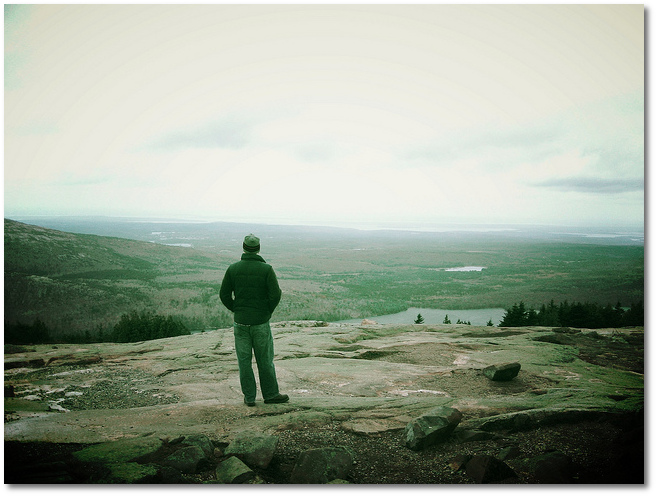
\includegraphics[width=.52\textwidth]{me} \end{center}

\begin{center} For corrections or to contact me, please \href{http://alan-taylor.org}{visit my website}.\end{center}



\mainmatter
\clearpage
\setcounter{page}{16}

%-----------------------------------
% ANNOTATING READINGS
%-----------------------------------


\chapter{Annotation \& Critical Reading}

\begin{quote} \small There is something predatory, cruel even, about a pen
suspended over a text. Like a hawk over a field, it is on the lookout for
something vulnerable. Then it is a pleasure to swoop and skewer the victim with
the nib’s sharp point. The mere fact of holding the hand poised for action
changes our attitude to the text. We are no longer passive consumers of a
monologue but active participants in a dialogue.

\textemdash Tim Parks,
"\href{http://www.nybooks.com/blogs/nyrblog/2014/dec/03/weapon-for-readers/}{A
Weapon for Readers}"

\end{quote}

In college you will encounter demanding texts of great complexity. You will be
asked to engage these texts critically and to challenge the thinking and conclusions of others. You will also have to retain an extraordinary amount of information and recall it later. To thrive in this environment you will need to develop some new habits and strategies. The most basic, and most important, of these are a formal procedure for the \textbf{annotation of texts} and the creation of \textbf{critical summary notes}. 

\section{Annotating texts}

Analysis requires breaking an argument down into smaller parts so that you can
understand how those parts work together to make the whole. The best way to
begin this process is to annotate texts as you read them by using a system of symbols and marginal notes made on the document itself. There is no right or wrong way to mark up a text, but you should develop
a system that you are comfortable with and try to stick with it. Writing while
you read will help you stay focused and read critically. In fact, I would argue
that if you are not writing while you read\textemdash by putting it into your
own words through annotation, \hyperlink{summary}{\color{Ahrenge}{summary}}, \hyperlink{paraphrase}{\color{Ahrenge}{paraphrase}}, and \hyperlink{quotation}{\color{Ahrenge}{quotation}}\textemdash then you are not reading critically at all.

Your objective in annotation is to flag the key elements of a piece of
writing\textemdash such as the thesis, argumentative points, and key pieces of
evidence. This kind of work serves two purposes. First, it helps you maintain a
critical focus as you read. Second, it helps you later if the text must be used for study or your own writing.

During my annotations I always flag a number of
things. I underline the thesis once I find it and I place large dots
next to pieces of evidence or statements being used to support the
thesis. I always place keywords or a short statement next to each paragraph,
aiming to create a "micro summary" of the content. I use check marks or
exclamation points next to statements that I find important or noteworthy.
Sometimes I draw arrows to connect parts of the essay that seem related to me in
some way.

In addition to flagging and summarizing a text's key ideas and arguments, I also ask
questions in the margins or note places where I become confused. This is helpful
later, on my second reading, since I can pay more careful attention to the
passages that gave me trouble. I also write my thoughts as they occur to me and
state objections to things that seem problematic or wrongheaded. Sometimes I try
to connect an idea in one text with the idea(s) in another text I have read. Making these sorts of connections is a central feature of the kind of thinking and writing you will do in college.

As you can see from the example here to the right, the process of annotation
keeps me engaged, active, and alert\textemdash key components in critical
thinking.

\begin{center} 
\begin{figure}
\href{https://github.com/stockphrase/OpenHandbook/blob/master/Chapters/images/Annotation1.jpg?raw=true}{\includegraphics[scale=.135]{Annotation1.jpg}}
\end{figure}

%\href{https://github.com/stockphrase/OpenHandbook/blob/master/Chapters/images/Annotation1.jpg?raw=true}{\includegraphics[scale=.135]{Annotation1.jpg}}

\end{center}

\subsection{The false allure of the highlighter}

Students often associate critical thinking and a general studiousness with the use of a highlighter. However, I'd like to question this practice a bit. Compare the following selection from a student's course reading to the annotation practices outlined above:

\bigskip

\begin{tcolorbox}[enhanced,width=4.2in,left=.4in, right=.4in,
   drop fuzzy shadow southeast,
    boxrule=0.4pt,sharp corners,colframe=black!80!black,colback=white!10]

\smallskip

\begin{flushright}

%\rule{4cm}{.7pt}

{\economica \emph{Biosystems} 31 (1993) \hspace{6pt} 238}

\end{flushright}

{\small
\begin{doublespacing}

\hspace{.5cm}At the heart of the environmentalist worldview is the conviction that \hl{human physical and spiritual health depends on sustaining the planet in a relatively unaltered state}. \hl{Earth is our home in the full, genetic sense,} where humanity and its ancestors existed for all the millions of years of their evolution. \hl{Natural ecosystems\textemdash forests, coral reefs, marine blue waters\textemdash maintain the world exactly as we would wish it to be maintained.} Our body and our mind evolved precisely to live in this particular planetary environment and no other. \hl{When we debase the global environment and extinguish the variety of life, we are dismantling a support system that is too complex to understand, let alone replace}, in the foreseeable future. . . . We run the risk, conclude the environmentalists, of beaching ourselves upon alien shores like a great confused pod of pilot whales.

\bigskip


\end{doublespacing}}

\end{tcolorbox}

There are a number of problems worth noting here about the practice of highlighting while reading: 

\begin{itemize}

\item First, your objective when you read something should be \emph{to avoid having to read it again} (unless, of course, you would enjoy doing so). Highlighting important portions of a text, as this student has done, only signals that the highlighted bits were important to the reader at the time of the reading. But to discover \emph{why} they are important or \emph{what} the highlighted portions mean, the student will be forced to read the text again. Busy students studying for multiple midterms do not have time to re-read entire books or articles.  

\item Secondly, highlighting works against critical thinking by casting the reader in the passive role of information consumer. As \href{http://libcat.dartmouth.edu/record=6773185}{Keith Hjortshoj argues}, highlighting merely "emphasizes the authority of the text: what its author says, believes, or knows. The practice therefore leads you toward memorization and repetition, not toward interpretation, inquiry, or criticism" (41). While recalling information at a later time is important, this is not the sole purpose of reading. Critical reading also involves a process of evaluating, questioning, and interpreting the text\textemdash activities that highlighting severely limit.

\item Thirdly, highlighting doesn't help you place the information into your long-term memory. \href{https://sites.udel.edu/victorp/files/2010/11/Psychological-Science-2014-Mueller-0956797614524581-1u0h0yu.pdf}{Recent  
research} suggests that \href{https://www.scientificamerican.com/article/a-learning-secret-don-t-take-notes-with-a-laptop/}{taking notes by hand} results in a significant boost to information retention.

\item Finally, highlighting doesn't help you understand the structure of an argument\textemdash the main goal of any critical analysis. Arguments all have a certain structure: there is a main idea supported by a series of claims, reasons, and pieces of supporting evidence. The highlighter \emph{fails to reveal this structure}. Flagging key structural features of arguments (as described above in the process of annotation) will dramatically reduce the time it takes to study and will be of significant help in your writing as you make use of the texts in question.

\end{itemize}

\subsection{Annotation strategies}

Since you have likely never engaged a text in such a manner, here are some
strategies that you might consider as you develop a process for annotation and
critical reading:

\begin{itemize} \item \textbf{Use a symbol system}. Develop a system of symbols
to flag important aspects of a reading. Mark significant elements within the
text such as the thesis, argumentative claims, and evidence. Also note when a
text references other texts, authors, or events. Note places where you become
confused or uncertain; later, in a second reading, you can give extra attention
to these portions of the text.

\item \textbf{Interrogate the text}. Be ruthless. Be rigorous. Ask questions
back to the author in the margins of the text. Challenge the conclusions and
arguments that he or she presents by making ones of your own.

\item \textbf{Summarize}. Write keywords or make "microsummaries" in the margins
next to each paragraph. Later, you will not have to re-read the entire document
to find your place. These can be especially useful if you later use this text in
your own writing.

\item \textbf{Connect}. Find connections between the reading and others within
the course or your broader reading experience. Develop the capacity to bring
other texts into dialogue with each other, imagining writing and reading as a
form of social interaction. \end{itemize}



\chapter{Critical Notes}
\hypertarget{notes}{}

\begin{quote} \small "We believe the best way to work on a difficult text is by
rereading . . . but you can also work on the difficult text by writing, by taking
possession of the work through sentences and paragraphs of your own, through
summary, paraphrase, and quotation, by making another writer’s work part of your
work" (12).

\textemdash Bartholomae and Petrosky, "Introduction." \emph{Ways of Reading: An
Anthology for Writers}

\end{quote}

\section{Taking Critical Notes}

One objective of the annotations described in the previous chapter is to help you create a \textbf{critical outline} during a subsequent reading. The objective in the critical
outline is to boil the entire argument down to its essence, without losing any
significant detail. The name of the game here is \textbf{reduction}: take
something complex and unwieldy and turn it into something small and useful for
study or your own writing. There is a real art to this, and you will become
better and faster at this as you practice. Over time, you will train your mind
to operate in such a way that you will perform these tasks almost unconsciously
as you read. These critical notes will be indispensable study aids. They will
also dramatically your writing.

These critical summaries are comprised of nothing more than \hyperlink{summary}{\color{Ahrenge}{summary}}, \hyperlink{paraphrase}{\color{Ahrenge}{paraphrase}}, \hyperlink{quotation}{\color{Ahrenge}{quotation}}, and your own observations and
questions. Quote only the most important, memorable language. Summarize or
paraphrase the rest in as objective a manner as possible. Take great care when
summarizing or paraphrasing; if your work is too similar to the original text
and is used later in your own writing, \emph{you may inadvertently commit
\hyperlink{plagiarism}{\color{Ahrenge}{plagiarism}}}, a serious academic
offense. Therefore, carefully place the writing of others into your own words
and \hyperlink{citation}{\color{Ahrenge}{cite the page numbers}} you reference in your notes.

As you write this critical outline you will not only try to reduce the main
points of the argument, you will also ask questions and make observations of the
text. You should note the argumentative points that you find yourself strongly
agreeing or disagreeing with and your reasons for doing so. You might see a
logical inconsistency or want the author to provide more evidence for his or her
claims. You might make a note to perform some research at the library or on the
Internet on an unfamiliar concept or event mentioned in the argument.
Ultimately, however, you will want to determine if the argument you have read is
persuasive and provide the reasons why.

At the end of this process, you should have a simplified\textemdash but
objective and accurate\textemdash version of the essay that has been ruthlessly
cut down to its bare essentials as well as a number of critical observations,
questions, and ideas that have emerged in your process of reading. By the time
you reach this stage and read over your notes, you will have taken great strides
toward mastering the information or argument. Of course, if the text is difficult, you may have to repeat the process until you have a breakthrough. I cannot emphasize enough how helpful and important this process is. It will help you come to a greater understanding of the text’s claims and weaknesses while also activating your long-term memory. 

Finally, to be a successful student and scholar, you will need to \hyperlink{joyofreuse}{\color{Ahrenge}{create a system for organizing and retaining these annotations and notes}} for later use. You might use a series of organized folders on your computer or some kind of filing system in manila folders. Whatever works best for you. Retaining all of this hard work will be of great importance to you later, particularly as you engage in large \hyperlink{academicresearch}{\color{Ahrenge}{research}} projects. As I describe in the next chapter, being a scholar\textemdash or just a great student\textemdash involves reusing and re-purposing prior work and information. 
 
\smallskip

\begin{center}
\begin{tcolorbox}[colframe=oyster, coltitle=black, sharp corners, title=\ding{52} Note]

\href{https://sites.udel.edu/victorp/files/2010/11/Psychological-Science-2014-Mueller-0956797614524581-1u0h0yu.pdf}{New research} suggests that taking notes by hand, \href{https://www.scientificamerican.com/article/a-learning-secret-don-t-take-notes-with-a-laptop/}{rather than using a computer}, aids memory and improves student performance.

\end{tcolorbox}
\end{center}


\subsection{Critical notes strategies}

Developing a process for making critical notes is perhaps the most important new
habit you will need to be successful in college. Here are some strategies or
principles that may guide your efforts:

\begin{itemize} \item \textbf{Reduce}. Use \hyperlink{summary}{\color{Ahrenge}{summary}}, \hyperlink{paraphrase}{\color{Ahrenge}{paraphrase}}, and \hyperlink{quotation}{\color{Ahrenge}{quotation}} to reduce an argument to its bare
bones.

\item \textbf{Engage}. Grapple with the ideas and arguments in the text. Ask
questions and make observations. You should note the argumentative points that
you find yourself strongly agreeing or disagreeing with and your reasons for
doing so. You might see a logical inconsistency or want the author to provide
more evidence for his or her claims. You might make a note to perform some
research on an unfamiliar word, concept, or event mentioned in the argument.

\item \textbf{Protect yourself}. Be scrupulous when you \hyperlink{summary}{\color{Ahrenge}{summarize}} and \hyperlink{paraphrase}{\color{Ahrenge}{paraphrase}}
source materials in your notes by ensuring that you use your own language and
sentence structure. A lazy mistake at this stage may cost you dearly later if
you inadvertently \hyperlink{plagiarism}{\color{Ahrenge}{plagiarize}} material. Don't forget to meticulously cite the page numbers of all the information you include in your notes.

\item \textbf{Save your work.} You will need to \hyperlink{joyofreuse}{\color{Ahrenge}{create a system for organizing and retaining these annotations}} and notes for later use. You might use a series of organized folders on your computer or some kind of filing system in manila folders. Whatever works best for you. 

\end{itemize}




\hypertarget{joyofreuse}{}

\chapter{The Joy of Reuse (Save Your Work)}


\section{Save all your work}

Most students complete their school work, turn it in to their professor, then never think of it again. These efforts then cross the event horizon into the black hole of a computer hard drive, never to emerge again. If this sounds like your standard practice, consider a change now that you've arrived at college. When you write something (essays, notes, reports, projects, code), or when you use something (course readings, research, data), keep a copy of it in some organized folder system so you may return to it in the future. 

Taking the time to meticulously save all this work may sound counterintuitive\textemdash the class is over, right? But that essay you wrote freshman year, the notes you took on a scholarly article, the readings you dutifully annotated in your history class, may be very useful to you in some future project that you can't anticipate now. And while it is important to save your finished work, it is also critical that \emph{you save the research or notes or data that contributed to that project as well}. Try, as best you can, to capture \emph{all} of the inputs that led to your finished work and save it in some organized way. Successful scholars and students return to prior work all the time\textemdash reshaping, repurposing, and extending prior efforts. They understand that knowledge is cumulative: it accretes and deepens over time, often by building on what came before. \emph{This is the joy of reuse}. Summarily tossing all of your work into the black hole forces you to start over again and again. 

\section{Staying organized}

To retain your work and stay organized, you might use a simple paper system made up of manila folders. Or you might use a hierarchical folder system on your computer, organized by class, project, or term. Alternatively, you might embrace a powerful bibliographic manager like \href{www.zotero.org}{Zotero}. Whatever you choose, create a system for staying organized and stick with it. 

\subsection{A poor file-saving strategy}

I assume that most students today will embrace an electronic system to manage their workflows, take notes, and compose texts. Let's imagine two archive systems to store this typical scholarly work. Consider the following file structure:

\medskip

{\large
\begin{tikzpicture}%
  \draw[color=black!60!white]
  \FTdir(\FTroot,root,/){       % root: parent = \FTroot
    \FTdir(root,etc,\textbf{My Documents}){       % normal dir: (parentID, currentID, label)
      \FTfile(etc,Notes.docx) 
      \FTfile(etc,Notes2.docx) 
      \FTfile(etc,Nosetalgia.mp3) 
      \FTfile(etc,Essay.docx) 
      \FTfile(etc,Revision.docx) 
      \FTfile(etc,syllabus.pdf) 
      \FTfile(etc,hack-dartmouth.py)
      \FTfile(etc,MyDogRex.jpg) 
      \FTfile(etc,ideas.docx)       % file:       (parentID, label)
      \FTdir(root,Stuff,\textbf{Stuff})
    }
  };
  \end{tikzpicture}  
}
 
\begin{center} \{ \hloy{A poor file-saving strategy} \} \end{center}

\noindent The strategy represented here breaks down very quickly for two reasons. First, after a few weeks of accumulating notes, readings, research, and other important documents, a system with no hierarchically organized folders becomes a confusing and unhelpful jumble. Secondly, the choices for naming the files actively resist discovery and recognition. What, for example, is the subject of \hloy{Notes.docx}? What class was it from? What lecture? What project were these notes taken for? Of the many essays you wrote, which one is \hloy{Essay.docx}? And \hloy{Revision.docx} is a revision of what, precisely? A year from now you won't remember, but you may very well care at that time. Unfortunately, the folder into which you've dumped these files will have swelled to a debilitating size that will disrupt any attempts to make use of your hard work. 

\subsection{A better file-saving strategy}

Instead of this haphazard and unhelpful approach, each time you place an artifact in your archive, think about your future self who will want to find something quickly, with minimal effort. An important first step in this process is to adopt some kind of logical foldering structure that quickly reduces the effort of finding a particular item. You should make considered and thoughtful decisions about your archive's structure. Perhaps you will choose to organize your work by year, or term, or class, or project. There are pluses and minuses to any organizational schema, but changing things up later is difficult, so choose wisely. 

Perhaps the most critical step in the construction of your scholarly archive is to adopt a \textbf{strict naming convention} for your folders and files. Keep in mind sociologist Kieran Healy's \href{https://kieranhealy.org/files/papers/plain-person-text.pdf}{helpful advice} that a "file or folder should always be able to tell you what it is" (7) without having to actually open it. Taking this sound advice, we might revise the previous filing strategy like this:

\medskip

{\large
\begin{tikzpicture}%
  \draw[color=black!60!white]
  \FTdir(\FTroot,root,/){       % root: parent = \FTroot
    \FTdir(root,My Documents,\textbf{My Documents}){       % normal dir: (parentID, currentID, label)
      \FTdir(My Documents,Courses,\textbf{Courses})       % file:       (parentID, label)
      \FTdir(Courses,Writing,\textbf{Writing 2-3-F19}){
        \FTfile(Writing,notes-Percy-10-28-19.docx)
        \FTfile(Writing,notes-Freire-11-5-19.docx)
        \FTfile(Writing,Essay1-draft1-9-07-19.docx)
        \FTfile(Writing,Essay1-draft2-9-15-19.docx)
        \FTfile(Writing,WR23-syllabus.pdf)
        \FTdir(Courses,CS1,CS1-F19){
        \FTfile(CS1,hack-dartmouth.py)
    	\FTdir(root,Music,\textbf{Music}){
    	\FTfile(Music,Pusha-T-Nosetalgia.mp3)
    	\FTdir(root,Photos,\textbf{Photos}){
    	\FTfile(Photos,MyDogRex.jpg)
    
      }
      }}}}
  };
  \end{tikzpicture}
}

\begin{center} \{ \hloy{A better file-saving strategy} \} \end{center}

Your system will obviously become far more complex than the simplified example presented above. (You might, for example, want to create subfolders within a class to further organize your files). However, the key features of a good filing system are detectable here: 1) there is a logical structure to the organization, using course names and file types to determine the names of the folders and 2) the naming convention for the folders and files tell you exactly what they are without having to open them. There is no right or wrong way to make a filing system, and one size will not fit all. You will have to determine for yourself what system makes sense to order all your work and research. 

\section{Very Large Filing Systems}

Most students would be fine if they use the simple filing system described above, where folders are determined by course or term. But if you have an expectation of a very large file system, or if you plan to share a file system with other researchers, you should consider a slightly different approach to the naming of files and folders. Large collections of files are quite difficult to manage; this is especially true when additional researchers are involved with saving and editing files in the shared directory. Special care in the naming of files and folders is critical here to avoid confusion and lost data. 

\begin{itemize}
\item While each project is different and will require its own approach, there are two best practices that should be followed in any shared research repository: a plaintext \textbf{README} file in each project directory and \textbf{a strict naming convention} for files and folders, described below.  
\end{itemize}

\subsection{An example README file}

A README file is simply a plaintext file that contains general information about a project. It functions like a roadmap that helps other researchers orient themselves to a new project and helps them coordinate their efforts more easily.  Information in a README might include the following:

\begin{itemize}
\item A short overview of the project.
\item The names and contact information of the researchers.
\item An inventory list of all the data or documents within a directory (with a short description of what they are). 
\item If the project involves software: a description of installation, dependencies, how to report bugs, licensing, etc.
\item Descriptions of file versions, if they are revised in some way.
\item If there are multiple subfolders (as in the example at right), those folder paths should be clearly indicated to show their location and contents.
\item A dated list of updates to the project as they occur. 
\item Suggested naming conventions for files and subfolders.
\item Descriptions of how other interested researchers can join you and your work.

\end{itemize}

\begin{center}
\begin{tcolorbox}[colframe=oyster, coltitle=black, sharp corners, title=README.md]

\textbf{RESEARCH PROJECT ALPHA}

\medskip

[Include an explanation of project]

\medskip

\textbf{\# Researchers}

\textbf{-} Jeff Goldbug: {\color{green}jeff.g.goldbug19@dartmouth.edu}

\textbf{-} Alain Frenchy: {\color{green}alain.frenchy@stanford.edu}

\textbf{-} Chloe Vinyl-Siding: {\color{green}chloe.vinyl-siding@gmail.com}

\medskip

\textbf{\# Data Inventory}

\smallskip

{\color{green}\textbf{/ProjectAlpha/Data/:}}

- \textbf{201907-EditData.xlsx} (data on edits)

- \textbf{201907-EditData.RData} (R dataset file)

- \textbf{201907-GrantLetter.docx} (Letter to Rich Foundation)

- \textbf{201907-Visualization.py} (Data visualization program)

- \textbf{201910-VisualizationV01.py} (Update; bugfix \#14)

- \textbf{201911-VisualizationV02.py} (Update; bugfix \#15)

. . . \medskip

\textbf{\# Documents}

{\color{green}\textbf{/ProjectAlpha/Docs/:}}

- \textbf{201910-Bibliography.docx} (Project bibliography)

- \textbf{201910-Presentation.pptx} (Class presentation)

\medskip

\textbf{\# Updates}

- 20191012: Updated bibliography entries

- 20191028: Update to visualization program

- 20191103: Update to visualization program

\end{tcolorbox}

\end{center}

\subsection{File-naming advice}

Avoid using spaces or underscores in the naming of folders, as some computer systems or programs will have difficulty with them. Instead, use CamelCase and dashes to make the folder and file names more human-readable.

\subsection{Naming top-level project folders}

\begin{itemize}
\item \hloy{\textbf{/} ProjectAlpha} 

\hspace{.25cm} - Project name in CamelCase.

\item \hloy{\textbf{/} 201908-ProjectAlpha} 

\hspace{.25cm} - Date in YYYYMM format will help with sorting in file managers.

\item \hloy{\textbf{/} ProjectAlpha-AT} 

\hspace{.25cm} - Author initials may be included, if needed.
\end{itemize}

\subsection{Naming files}


\begin{itemize}

\item \hloy{YYYYMM-FileName.docx} 

\hspace{.25cm} -Prototypical example.

\item \hloy{201910-FileNameV01.docx} 

\hspace{.25cm} - File revision/version; \emph{use two digits with leading zero for proper sorting in file managers}

\item \hloy{201910-FileNameDraft.docx} 

\hspace{.25cm} - A draft version

\item \hloy{201911-FileNameFinal.docx} 

\hspace{.25cm} - A final version

\item \hloy{201912-FileNameDraftAT.docx} 

\hspace{.25cm} - Include initials at the end of the file, if needed.

\end{itemize}

\subsection{A very large file system example}

{\large
\begin{tikzpicture}%
  \draw[color=black!60!white]
  \FTdir(\FTroot,root,/){       % root: parent = \FTroot
    \FTdir(root,etc,\textbf{ProjectAlpha}){       % normal dir: (parentID, currentID, label)
      \FTfile(etc,201907-WebScraper.py) 
      \FTfile(etc,201908-ProcedureManual.docx) 
      \FTfile(etc,201910-DataDump01.xls) 
      \FTfile(etc,201910-DataDump02.xls) 
      \FTfile(etc,201910-DataDump01Analysis.docx) 
      \FTfile(etc,201911-PublicTalkPresentation.pptx) 
      \FTfile(etc,201911-Visualization.rdata) 
      \FTfile(etc,201911-VisualizationV01.rdata)
      \FTfile(etc,201912-VisualizationV02.rdata) 
      \FTfile(etc,201911-VisualizationV03.rdata)  
      \FTfile(etc,. . .) 
      \FTfile(etc,README.md)      
      \FTdir(root,Stuff,\textbf{ProjectBeta})
    }
  };
  \end{tikzpicture}  
}

\section{Back up all your data}

All of this hard work of organizing will be for nothing, however, if you don't take pains to back up your data. \textbf{Please, I beg of you, back up all your data regularly and keep a copy separate from your main working computer}. There are heartbreaking stories of people losing years of work in a hard drive failure, theft, or house fire/flood. Few people are disciplined enough to back up their work regularly on their own initiative. Instead, you should embrace some kind of \href{https://www.jwz.org/blog/2007/09/psa-backups/}{regular, automated system} to ensure your work will survive any tragedy. 

\begin{itemize}
\item At some point in the future you will boot up your laptop and it will begin smoking, or be infected by ransomeware, or display the \href{https://en.wikipedia.org/wiki/Blue_Screen_of_Death}{BSoD}. You will have no backups. As you cry salty tears you will remember reading these words and not doing anything about it. \textbf{ -- I told you so}.
\end{itemize}
%%----------------------------------------------------------------------------------------
%	How to be a student
%----------------------------------------------------------------------------------------

\chapter{Relating to your Professors} 

One of the most difficult things to navigate at college is how to relate to your instructors. Here are a few marginally helpful things that may help you keep a good relationship with your teachers.

\section{Tactical errors with professors}

\begin{itemize}

\item \hloy{Timing is everything}. Asking your professor to meet and discuss your idea(s) for a project shortly before it is due reveals that you haven't started yet. There is a certain cutoff point after which you should not reveal such things to the person who will grade your work. While it is quite possible for a good student to write something amazing overnight, revealing this to your professor may not be to your advantage. 

\item \hloy{Did I miss anything important}? This is one of the most annoying questions professors hear. Never ask your professor if you "missed anything important" on a day you were absent. Yes, yes you did. It is all important. (And even if it's not, pretend that it is).

\item \hloy{There are no dumb questions}. It has been said that there are no dumb questions. But this is wrong. There is an amazing variety of dumb questions asked with a great deal of frequency. One you can easily avoid is asking something that is already thoughtfully covered in the syllabus. Ensure the question you have about the class isn't answered in the syllabus before you ask your instructor. Of course, if something in the syllabus is confusing or ambiguous, please ask for clarification. 

\section{Asking for extensions}

\item \hloy{Extensions are only occasionally justified}. Sometimes life intervenes in our plans and rudely sets us back. If you get hit by a bus or contract ebola, asking for a paper extension is a reasonable request. But generally it is a bad idea to request an extension unless you find yourself in a similarly extreme situation. Many faculty are reluctant to give extensions because of a duty to the principle of fairness: if one student is granted an extension, the other students who turned their work in on time are disadvantaged. Students have been known to turn in several large projects on the same day without requiring extra time. These students accomplish this feat by planning ahead, usually by mapping out all of their assignments for an entire term in a calendar, then starting early. And, for what it's worth, I know of at least one professor who, while granting extra time on occasion, always grades the resulting work much more stringently than if it had been turned in on time. 

%\item \emph{I'm too busy}. Asking for an extension because you are "too busy" with other classes or have other work due at the same time is not a good look for you. Your professor might conclude that you consider those other courses more important than hers. She might conclude that because that is exactly what you are, in effect, saying. 

\section{Office hour \emph{faux pas}}

\item \hloy{Avoid showing up at your professor's office when it is not office hours}. Professors are very busy with research, administrative duties, and class preparation. Many also have family obligations. If your professor is in her office and it isn't office hours, she isn't waiting for you. You can, of course, set up an appointment to meet with your instructor at a more convenient time. 

\item \hloy{ I know you're in there!} I can't believe I have to say this, but the student who shows up at a professor's office at an unscheduled time, discovers a locked door, then \emph{proceeds to knock on the door until the professor hiding inside opens it,} has just performed an incredible feat of self-immolation.

\item \hloy{Don't bogart your professor}. If a line of students form during an office hour and you have been interacting with the professor for quite some time, allow your fellow students to enter. You can always return to the line or ask for a separate appointment to continue the discussion. 

%\section{Honorifics and such}

%\item \hloy{What do you call your teachers}? Almost every year a student will ask me "What do we call you?" on the first day of classes. This is hard to answer. All of your teachers at Dartmouth have terminal degrees in at least one academic field. Usually this means a Ph.D. They publish books and articles. They are asked to give speeches and talk on television. For some faculty, this has become so related to their own sense of self-worth that they will visibly cringe if you call them "Bill" or, even worse, "Mr. Smith." Let's call this group the \textbf{Prouds}. A second group, although just as accomplished as the Prouds, are less dependent on their academic accomplishments to gain psychological uplift. They would actually \emph{prefer} if you called them by their first name in order to better signal a desire to close the distance between teacher and pupil. Let's call them \textbf{Brofs}. A third group, perhaps the most interesting of the bunch, are the \textbf{Pseudo-Brofs}. While they will look you directly in the eye and say "I don't care what you call me," or "call me Phyllis," in truth (for psychological reasons too complex to go into here) they crave the honorific "doctor" or "professor" even more than the Prouds. Now, students, what does this mean for you? It means that unless you love to court danger and/or have too much integrity to submit to authoritarian systems, the safe move is probably to call all your teachers "professor X" or "doctor X."


\section{Seeking help}

\item \hloy{Seek help, don't grub}. Your professors want to help you. Really, they do. \emph{But at some point, seeking help becomes a form of dependence}. Taken to extremes, your help-seeking becomes an avoidance of your own responsibility as a writer, a thinker, a student, a human. Over the years I have had many students who bring their work to me excessively and who want my approval on every edit of their written work. Obviously, the students who do this just want to do well, but consider what they lose in the bargain. At some point, the essay or project ceases to be the work of the student, as the line between authorship and critique first blurs and then becomes indistinguishable. The student has completely surrendered his right to think and know and argue \emph{on his own terms}, blithely giving away his freedom to an authority figure in the person of his teacher. College should be a series of experiences through which you \emph{gain ownership over your own thinking and define for yourself your ideas and values and meanings}. While your teachers are here to provide feedback, critique, and assistance, you should do your own work, think your own thoughts, write your own papers, and, through those experiences, become who you are.  

\section{Recommendation letters}

\item \hloy{Recommendation letters}. I have never turned down a student for a recommendation letter. I enjoy recommending my students to graduate programs, medical schools, and scholarship committees. Feel free to ask me, or any professor who knows you, for a letter. Just make sure that you ask early. Students who ask for letters with 12 hours notice do not usually get the best letters. It unnecessary to buy me coffee or lunch to secure one.

\end{itemize}

%\chapter{Course Policy FAQ}

\section{Can I email you an essay or draft when it is due?}
\begin{itemize}

\item {\Large \color{Ahrenge}\textbf{No.}} 
\end{itemize}

However, in order to prevent your essay from being late you may email a copy as a placeholder until you turn in a paper copy. This might happen if your printer fails or you spill coffee on your essay. Please ensure that the paper copy you hand in later is identical in very way to your electronic placeholder.


\section{Can I email you an essay for extra comments?}
\begin{itemize}

\item {\Large \color{Ahrenge}\textbf{No.}} 
\end{itemize}


I usually do not take requests for extra comments via email unless there is no other possible way a student can meet with me in person. \textbf{However, I am happy to discuss new drafts with students during office hours or at other times by appointment}. Considering how easy it is to attach a file to an email, almost every student would seek this additional help. As a result, I would be deluged with requests for help, often at the very last minute. These requests would become so numerous that it would be impossible for me to thoughtfully respond to them all. And it wouldn’t be fair to help some students and not others. \emph{More significantly, I think this practice also sends the wrong message that I am your personal editor}. That really isn’t my job.

\section{Can I bring my laptop to our office meeting?}
\begin{itemize}
\item {\Large \color{Ahrenge}\textbf{No.}} 

I try to save the trees as much as possible. However, I have discovered that under these circumstances students often type the words that I say directly into their papers. This potentially blurs the line between critique and authorship. Since it is important that you do your own work, it is best to avoid this problem/temptation by using a hard copy.
\end{itemize}

\section{I can't make office hours; can we meet another time?}
\begin{itemize}
\item {\Large \color{Ahrenge}\textbf{Yes.}} 

I will be happy to accommodate students whose schedules conflict with my office hours. Contact me and we can work out the details. If we are unable to find a time that works for both of us, the \href{https://students.dartmouth.edu/rwit/}{RWIT} is another excellent option.
\end{itemize}

\section{Can I have an extension?}
\begin{itemize}
\item {\Large \color{Ahrenge}\textbf{Sort of.}} 

I must be fair to all of my students. If I give an extension to one student, the other students who turned in their essays on time are disadvantaged. For that reason I deduct a full letter grade for each day an assignment is late. Take as much extra time as you wish; however, you should be prepared to face the consequences. Of course, if you have a serious emergency that prevents you from completing work, I will be happy to work out a new due date.
\end{itemize}

\section{Do you have a grading rubric?}
\begin{itemize}
\item {\Large \color{Ahrenge}\textbf{Yes and No.}} 

I do not have a formalized rubric to explain the exact nature of the A, B, C, D, and F essay. However, \hyperlink{good-writing}{\color{Ahrenge}{here is an explanation of what I value in good academic writing}}. 

\end{itemize}

%----------------------------------
% On Good Writing
%-----------------------------------

\hypertarget{good-writing}{}

\chapter{What is Good Writing?}


Academic writing takes many forms. However, all \emph{good} academic writing shares several basic characteristics:

\begin{itemize}

\item Good academic writing always contains a \textbf{strong thesis statement}: an idea, stated as an assertion, that is the work's central focus.
\item Good academic writing is \textbf{organized}: each \hyperlink{organization}{\color{Ahrenge}{paragraph}} builds upon the one before it, creating a strong sense of purpose. The paragraphs themselves are unified, generally pursuing a single idea that helps support the \textbf{thesis}. Each paragraph should use a strong \hyperlink{organization}{\color{Ahrenge}{topic sentence}} that clearly indicates the subject of the paragraph.
\item Good academic writing has \textbf{elegant and logical transitions} between paragraphs and ideas.
\item Good academic writing shows an awareness of the needs of its particular \hyperlink{audience}{\color{Ahrenge}{audience}} by contextualizing the ideas, texts, authors, debates, or histories that are discussed within it.
\item Good academic writing is \textbf{relevant, useful, and interesting} to its imagined \hyperlink{audience}{\color{Ahrenge}{audience}}.
\item Good academic writing \textbf{skillfully uses evidence} to support claims and it \hyperlink{sources}{\color{Ahrenge}{properly credits outside sources with citations}}.
\item Good academic writing is \textbf{precise, clear, and concise}.

\end{itemize}



%-------------------------------------------------------------------------- %
 % TYPES OF WRITING AT THE COLLEGE LEVEL %--------------------------------------------------------------------------

\chapter{Types of College Writing}

Most students are trained in high school to write what is known as a
five-paragraph essay\textemdash a form of writing containing an introduction,
three paragraphs of support, and a summary conclusion. In that it encourages
students to think about introductions, structure, organization, paragraphing,
evidence, and reasoning, the five-paragraph essay is good training for novice
writers. However, this particular rhetorical form is \emph{extremely} limiting:
only certain, rather paltry, thoughts and ideas may be placed within a five
paragraph structure. 

Your college coursework will require that you reach for rhetorical forms of an
entirely different nature. Little of the thinking you will be challenged to do
in college will fit within the constraints of the five-paragraph essay. Big
ideas, complex reasoning, and deep inquiry will require more sophisticated structures.
Rather than force all of your reasoning and inquiry into a preformulated and
supposedly universal structure, \emph{you will be asked to embrace the idea that
the formal properties of a piece of writing are determined by the particular needs of the
argument}. Thus, the shape of your reasoning will determine the essay's form. Furthermore, every discipline has its own particular way(s) of writing; as you
progress through your coursework you will become more familiar with how your
chosen field of study presents its own kind of academic discourse.

While academic writing takes on many forms, the following are the most common
modes of writing you will encounter. However, it is perhaps misleading to
present these various modes of academic writing as discrete things. Please
understand that there are no definite lines between these various kinds of academic
writing, and it is uncommon to write in one mode exclusively. The rhetorical tasks
you face in college will often require you to \emph{combine these modes in
various ways within a single piece of writing}. For example, an argument paper
will often involve synthesis and analysis, a research essay may use one or more
theories, and a theory paper might use close reading and analysis.

\hypertarget{argument}{} \section{Argument}

An argument paper requires you to make a claim about a debatable issue and then
defend that claim using evidence and reasoning. Virtually all academic writing
is argumentative in nature. Argumentative essays generally begin with an introduction
that explains the context for the argument and the specific issue, problem, or
question that the paper will address. Typically, the author of an argument will
use the end of the introduction to present a \hloy{thesis}\textemdash the main
idea or claim of the essay. However, this is not always the case. For example,
one argumentative form known as the "exploratory essay" replaces the thesis with a
question that is used to initiate an inquiry into an issue or problem. Typically, the
thesis appears near the end of this kind of essay, as the culmination of a process
of reasoning and inquiry.


\hypertarget{responseessay}{} \section{Response}

A response paper gives you free license to respond to a text without guidance.
Rather than a prompt or prescribed approach given to you by a professor, a
response paper allows you to engage a text on your own terms and write from your
own perspective.

While a response paper allows you to write about something you choose, your
effort should not be an impressionistic one where you only talk about your
personal feelings\textemdash what you like or dislike about the text. Rather,
you should seek to \emph{evaluate} and \emph{engage} the claims and ideas you
find in the text. Thus, a response is always argumentative in nature in that you will make 
claims and use reasoning and evidence as support.

Your response may seek to take issue with some of the thinking or reasoning put
forth in the reading. However, a good response doesn't just say "I agree with X"
or "I disagree with Y." Instead, \emph{explicit reasons are stated and
explanations are made that challenge or support the writer's ideas}. A good
response essay might alternatively attempt to forge a connection between two or
more texts by demonstrating a relationship between the ideas or arguments
involved\textemdash contrasting, comparing, and evaluating the claims or ideas
in the texts. For example, how might Author A respond to Author B? How
do their views compare? Can their views be reconciled? Is one view superior?

\section{Exposition} An expository essay is one in which you report on, define,
summarize, clarify and/or explain a concept, process, idea, or text. Expository
essays involve several key patterns such as compare and contrast, cause and
effect, problem and solution, or definition. The purpose of this kind of
writing is to provide information to an audience unfamiliar with the subject or
to demonstrate for a professor that you have understood course material.

\hypertarget{synthesisessay}{} \section{Synthesis}

As the name suggests, synthesis essays emphasize \emph{combining} and
\emph{connecting}. Your focus in a synthesis essay is to explain to your
audience the ways in which two or more arguments or ideas relate to one another.

Students attempting synthesis for the first time often make the mistake of
organizing their essays by source. For example, this student might introduce two
authors in her introduction, summarize Author A, summarize Author B, then
conclude by noting the broad similarities and differences in the two authors'
thinking. This is \emph{not} synthesis.

In a synthesis essay it is generally best to organize your essay by \emph{topic} or
\emph{questions at issue} rather than by sources. Rather than try to summarize
the essays separately, a synthesis will attempt to discover the various things
that the authors discuss\textemdash the questions, ideas, and arguments they
have in common\textemdash then present those things in an organized and
meaningful way. Thus, your objective in a synthesis is to bring two or more
distinct sources into a relationship by explaining to your reader the various
ways in which the sources are in \emph{dialogue}.

To begin a synthesis, ask yourself the following questions about the readings
you plan to synthesize: \begin{quote} What are the positions, arguments, and
ideas that the source materials have in common? Are the authors all concerned
about the same problem(s)?  Are their arguments similar or do they differ? What
reasoning supports their arguments? Do they offer similar conclusions or are
there differences? \end{quote}

\noindent After answering these questions \emph{exhaustively}, write an essay
that examines the relationship between the various authors’ arguments, comparing
and contrasting their views.

Synthesis is very textual in nature: \emph{you must show explicit textual
evidence for each of the claims you attribute to the other authors}. Using
\hyperlink{summary}{\color{Ahrenge}{summary}},
\hyperlink{paraphrase}{\color{Ahrenge}{paraphrase}}, and
\hyperlink{quotation}{\color{Ahrenge}{quotation}}, compare and contrast the
authors’ positions. Make sure to cite each of these appropriately. Use clear
\hyperlink{signalphrase}{\color{Ahrenge}{signal phrases}} to transition between
your presentations of the various author’s ideas or works.

\hypertarget{closereadingessay}{} \section{Analysis/Close Reading} Analytical
writing involves paying close attention to particular elements of a thing and
how those discrete elements work together to produce a whole. While analysis
always involves breaking things down and meticulously examining the particulars,
the ultimate goal of any analysis is to explain what something means or how it
works. In the case of literary criticism, for example, you might perform an analysis of a
poem and then attempt to explain its meaning to your audience.  Rather than
quote an outside authority, you will instead provide your interpretation
of the text \emph{using only the words of the poem itself as evidence}. This process is
often referred to as "close reading." While this process may be performed on a
poem or a scene in a novel, a close reading may also be made of a film
sequence, a piece of artwork, a photograph, a built structure, a tribal practice, or
even a new fashion trend.

In more scientific disciplines you might examine a collection of data, then
describe in detail how this information leads to a broader explanation, theory,
or conclusion. In all cases, the analysis you perform should be used to support
a strong \hloy{thesis}\textemdash an idea or that you want your audience to accept as
true.

\hypertarget{theoreticalessay}{} \section{Theoretical Writing} The theoretical
essay is one of the most common forms of academic writing. Using a theory is
like using a tool: you take it with you to your job of reading and interpreting
a text and use it to uncover ideas and shape thoughts. Sometimes people refer to
theoretical arguments as “lens” essays since you view the text(s) you are
analyzing through the theory you have chosen. Like a lens, the theory will color
the text, bring certain things into focus, and make others fade out of view.

We might, for example, use a feminist theory to examine a novel. In this case,
the theory would sensitize us to certain aspects of the text such as the power
relationships between the female and male characters or how social authorities
or institutions treat men and women differently. Alternatively, we might perform
a Marxist analysis which would cause us to study how social class and
disparities in wealth shape the narrative and the various characters' outcomes
in the fictional world they inhabit. But theory is not just for the analysis of
fiction. We might, for example, appropriate some economic, sociological, or
anthropological theory to analyze how people behave at the mall or use some
psychological model to explain the decision to join a fraternity.

There is an extraordinary variety of extant theoretical models that may be used
for the interpretation of texts, cultural forms, and various kinds of data. In
fact, every field of study uses theory in some way\textemdash from literary
criticism to the hard sciences. As you begin to specialize within a chosen
discipline of study, you will encounter the theoretical models that are
important for that discipline.

\hypertarget{researchessay}{} \section{Research}

A \hyperlink{academicresearch}{\color{Ahrenge}{research}} paper requires you to
draw on outside sources in addition to your own thinking. Research writing often
includes many of the kinds of writing described above. Indeed, research writing
involves a coordination of all of the previously mentioned skills and rhetorical
modes. For example, your research paper may involve one or more theories,
perform various kinds of analysis, synthesize the thinking of many other writers
or thinkers, and make one or more arguments.

When you make an academic argument, you are often entering a conversation that
existed long before you appeared. When you write, you must remain mindful of the
conversations that came before and nestle your views within those that already
exist. In short, you must demonstrate that your ideas have a \emph{context}.
This is where \hyperlink{academicresearch}{\color{Ahrenge}{research}} comes into
play. Before you can responsibly offer your views, you must know what the
critical conversation is, what arguments are being made, and what questions are
important (or irrelevant) to the debate.

Properly done, \hyperlink{academicresearch}{\color{Ahrenge}{research}} ensures
that what you write is a true contribution to the ongoing discussion, and not a
pointless exercise in repetition. The whole point, after all, is to move the
scholarly conversation further down the road.

%----------------------- % Audience %-----------------------
\hypertarget{audience}{}

\chapter{Audience}

\begin{quote} \small [A] work of rhetoric is pragmatic; it comes into existence
for the sake of something beyond itself; it functions ultimately to produce
action or change in the world; it performs some task. In short, rhetoric is a
mode of altering reality, not by the direct application of energy to objects,
but by the creation of discourse which changes reality through the mediation of
thought and action. The rhetor alters reality by bringing into existence a
discourse of such a character that the audience, in thought and action, is so
engaged that it becomes mediator of change (3-4).

\textemdash Lloyd F. Bitzer, "\href{http://www.jstor.org/stable/40593346}{The
Rhetorical Situation}." \end{quote}

\section{Constructing the Audience}

Everything we write has an audience\textemdash the person or people we address
with our words. Even a private journal is addressed to a future version of the
writer's current self. To a large degree these audiences will determine what we say and how we say it.

It is easy to jump too quickly to the immediate purpose of our
writing\textemdash the idea we want to articulate or the viewpoint we hope to
convince others to adopt. In doing so we forget that \emph{how} we say
something is as important as \emph{what} we say, particularly when we address
people who don't share our values, culture, or life experiences. The presentation of our
arguments\textemdash the kinds of evidence we use to support it, the words we
choose to articulate it\textemdash must be tailored for our audience if we hope
to be successful.

The nature of audiences is often elusive and complex. We may never completely understand the character and motives of our audience members; this imperfect knowledge presents a great challenge for writing arguments. Your audience members may hold views or beliefs that, while quite opaque, greatly determine receptiveness to your message. And in some cases your audience may be completely unknown to you\textemdash for example, if you write for the web. Thus, imagining the audience for your message is often not an easy task. It is something that you will have to make a judgment about using whatever evidence you happen to possess at the time. 

Before you write anything, carefully analyze those people whom you desire to
persuade. To the best of your knowledge, take an inventory of what you know about the audience (or audiences)
you plan to address in your writing. This analysis should give you 
insight into how best to present your thinking, reasoning, and evidence. You might begin such an audience analysis by asking questions such as these: \begin{itemize}

\item Who is your audience or audiences? 
\item What are their values? 
\item What educational background(s) do they have? 
\item What political views do they hold?
\item What ideas or commonalities do you share with them? 
\item What does your audience already know about the topic you plan to present? 
\item What form will your audience expect that your writing will take? (For example, if the writing occurs within a specific academic discipline, your writing will need to adopt to the \hyperlink{citation}{\color{Ahrenge}{preferred style}} for that discipline: MLA, Chicago, APA, etc.)

\end{itemize}
\noindent Questions like these can help us imagine the audience we address in
our writing and gain a sense of the rhetorical situation we face. This kind of
intelligence will help us make good decisions about many aspects of the writing
process such as organization, diction, style, and evidence.

\section{Persuading the Audience} 

While there are many types of writing, the kind you will do in college is largely concerned with \emph{argumentation} and \emph{persuasion}; it is a form of reasoned discourse designed to change the audience's mind or cause them to adopt some new idea or plan of action. As you analyze your audience with these and other similar questions, imagine how these particular people will respond to the argument(s) you plan to present to them. For example:

\begin{itemize}

\item What sorts of constraints do you envision in getting your audience to accept your
argument? 
\item If your intended audience already has known positions you
oppose, how can you work carefully to convince them that their views should
change? 
\item What sorts of things should you avoid presenting in your message?
\item What common values or beliefs can be used to make your views more
appealing and consistent with your audience's outlook? 
\item How can you establish rapport with your audience, based on what you know? 
\item How can you demonstrate that you are an authority on the issue or problem at hand?

\end{itemize}

\noindent Done properly, an audience analysis will help you craft your argument
more effectively, adopt a proper tone, use appropriate vocabulary, and avoid
any rhetorical missteps that may alienate your readers.

 \section{Addressing a broad audience}

In college your audience will most often be your professor and fellow class
members. However, when you write you should learn to address a broader, general audience.
This means that you will not take certain things for granted as you write and ensure
that you provide good contextual information designed to help your readers gain clear understanding. 

For example, while your professor knows the authors and readings he or she assigned in the class
very well, when you reference them in your writing you should take care to
introduce them, thus addressing a more expansive audience who may not
be familiar with the texts or authors in question. To illustrate, consider the following two
sentences:

\newpage

\textbf{1. As we talked about in class, Freire argues that banking can be undemocratic and oppressive.}

\begin{itemize} \item \hl{This sentence assumes that the audience knows
certain things, namely Paulo Freire, his essay, and class discussions}. However,
writing the sentence in this way excludes everyone who is not taking part in
this particular class. Imagine the confusion you would experience after reading
this sentence if you had not taken part in the discussion of this piece of
writing. You might wonder: What is "banking"? You mean my credit card company is oppressing me? Who is this Freire guy? Is he some authority I should trust? Where did he make this argument?
\end{itemize}

\textbf{2. In an essay entitled "The `Banking Concept' of Education," author and educator Paulo Freire argues that a widely practiced form of schooling that he terms "banking education" is oppressive and undemocratic.}

\begin{itemize}

\item \hl{The second sentence, however, attempts to include a much larger
audience by carefully introducing important contextual information}. By
providing the author's full name, his profession, the essay title, and the
definition of key terms, the audience will feel that they are being addressed by
your writing, rather than excluded. Further, they will gain important contextual
information that is needed for understanding.

\end{itemize}


%-----------------------
% Paragraphs and Topic Sentences
%-----------------------
\hypertarget{organization}{}
\chapter{Paragraphs \& Topic Sentences}

\begin{quote}
\small
I can remember picking up my father's books before I could read. The words themselves were mostly foreign, but I still remember the exact moment when I first understood, with a sudden clarity, the purpose of a paragraph. I didn't have the vocabulary to say "paragraph," but I realized that a paragraph was a fence that held words. The words inside a paragraph worked together for a common purpose. They had some specific reason for being inside the same fence.

\textemdash Sherman Alexie, "\href{http://articles.latimes.com/1998/apr/19/books/bk-42979}{Superman and Me}."

\end{quote}

A paragraph is a unit of text devoted to developing an idea. The idea is usually stated 
in a \textbf{topic sentence}. The topic sentence most commonly appears as the paragraph's first sentence;
however, in what is known as a periodic paragraph, the topic sentence will appear at the end.

Paragraphs should be unified. Every sentence in the paragraph should focus on the main idea expressed in the topic sentence. Further, the paragraph's individual sentences should be presented in a logical order and flow naturally from one to the other. It may be helpful to think of the paragraphs as miniature essays, each with their own thesis, development, and proof. 

\section{How can I make my paragraphs unified?}

\begin{itemize}

\item Identify the main idea of the paragraph then remove or revise any sentence that does not 
develop that main idea or repeats ideas offered in another sentence.

\item Consider the order of your sentences. Is there a reason why they are in the order 
they are, or do they need to be rearranged to make sense to a reader?

\item Think about employing some \textbf{transitions} at the beginning 
of some of the sentences. These will help you pinpoint the relationships between your 
ideas/sentences and thus clarify these relationships for your reader. To help guide your readers in understanding the relationships between the sentences of your paragraphs, you might use words like \emph{For example}, \emph{However}, \emph{Additionally}, \emph{Specifically}, \emph{On the other hand}, \emph{Obviously}, \emph{As a result}, \emph{In distinction to}, \emph{In other words}, \emph{Significantly}, etc.

\item Repeat key words to remind your audience of the paragraph's focus.

\end{itemize}
 
\section{Strong topic sentences}
Topic sentences function like a miniature thesis that communicates the purpose or main idea of a paragraph. It is important that your topic sentences are clear and accurately reflect the nature of the paragraph that follows it. 

Most commonly, topic sentences are strong, declarative statements that make a claim. The sentences that follow the topic sentence in the paragraph are used to support that claim. However, a topic sentence may also be a question. In this case, the sentences that follow the topic sentence are used to move toward a conclusion or further development or deepening of the question. 
 
\section{Example paragraphs}

This paragraph is part of a larger student essay performing a theoretical analysis of Wes Anderson's 1998 film \href{http://en.wikipedia.org/wiki/Rushmore_%28film%29}{\emph{Rushmore}}. The essay uses theoretical ideas borrowed from Brazilian educational theorist Paulo Freire. According the the author, the film's central character, Max Fischer, fails to live up to the standards for education that Freire articulates.

\subsection*{An incoherent paragraph:} 

\bigskip

\begin{tcolorbox}[enhanced,width=4.2in,left=.3in, right=.3in,
   drop fuzzy shadow southeast,
    boxrule=0.4pt,sharp corners,colframe=black!80!black,colback=white!10]

\medskip

{\small
\begin{doublespacing}

\hl{An incoherent paragraph:}\medskip

\hspace{.5cm}Liberation education culminates in an effort to change the world. However, according to Freire, this change must embrace a communitarian philosophy. This is what Max Fischer fails to understand. Max is keen to change the world, shaping it to his needs and wants, but he fails to understand Freire's imperatives on community, dialogue and consensus. The views, ideas, and values held by a community are used to change the world, not one individual's desire. Rather than shape the world \emph{with} others, Max insists on altering the world for himself alone.

\medskip

\end{doublespacing}}

\end{tcolorbox}

\begin{itemize}
\item \hloy{Analysis}: The \textbf{topic sentence} of the paragraph does not represent the true nature of the paragraph. The paragraph is about Max's failure to embrace a core idea expressed by Freire; however, the topic sentence suggests the paragraph will only discuss something called "liberation education." Further, the paragraph's sentences are not presented in a helpful or logical order.
\end{itemize}

\subsection*{Revised paragraph:}

\bigskip

\begin{tcolorbox}[enhanced,width=4.2in,left=.3in, right=.3in,
   drop fuzzy shadow southeast,
    boxrule=0.4pt,sharp corners,colframe=black!80!black,colback=white!10]

\medskip

{\small
\begin{doublespacing}

\hl{Revised paragraph:}\medskip

\hspace{.5cm}Although Freire argues that liberation education culminates in an effort to change the world, Max Fischer's efforts in this regard fail to embrace the philosophy of community that Freire demands. While Freire beckons us to become “transformers of [the] world” (73), he insists that it must only happen after a process of “dialogue”: an open exchange of ideas between equal partners (78-9). For Freire, these moments of co-inquiry are used to transform the world into a more democratic and free society (86). While Max is keen to change the world, he selfishly shapes it to \emph{his own needs and wants}, failing to understand Freire's insistence on community, dialogue, and consensus. Rather than shape the world \emph{with} others, as Freire recommends, Max insists on altering the world for himself alone.

\medskip

\end{doublespacing}}

\end{tcolorbox}

\begin{itemize}
\item \hloy{Analysis}: This revised paragraph uses the \textbf{topic sentence} to announce that the passage will focus on how Max Fischer fails to live up to a standard expressed by Freire. This new topic sentence reflects the nature of the paragraph much more faithfully. Furthermore, the author arranges the sentences so as to educate the audience about the Freire's theory before using it to criticize the actions of the film's main character, Max Fischer. The result is a more logical and intelligible paragraph.
\end{itemize}


%%----------------------------------------------------------------------------------------
%	STYLE
%----------------------------------------------------------------------------------------

\chapter{On Style} 

Some of the best advice on style I've ever read:

“This sentence has five words. Here are five more words. Five-word sentences are fine. But several together become monotonous. Listen to what is happening. The writing is getting boring. The sound of it drones. It’s like a stuck record. The ear demands some variety. Now listen. I vary the sentence length, and I create music. Music. The writing sings. It has a pleasant rhythm, a lilt, a harmony. I use short sentences. And I use sentences of medium length. And sometimes, when I am certain the reader is rested, I will engage him with a sentence of considerable length, a sentence that burns with energy and builds with all the impetus of a crescendo, the roll of the drums, the crash of the cymbals–sounds that say listen to this, it is important.”

--Gary Provost


%----------------------------------------------------------------------------------------
% WORKING WITH SOURCES
%----------------------------------------------------------------------------------------
\hypertarget{sources}{}


\chapter{Working with Sources}

\begin{quote} \small [A] quotation is a handy thing to have about, saving one the trouble of thinking for oneself, always a laborious business.

\textemdash A.A. Milne
\end{quote}

\begin{quote} \small The ugly fact is books are made out of books.

\textemdash Cormac McCarthy

\end{quote}

Academic writing always involves integrating the thinking of others into your own writing. There are only three ways that the words and ideas
of others may appear in your writing: \hyperlink{summary}{\color{Ahrenge}{summary}}, \hyperlink{paraphrase}{\color{Ahrenge}{paraphrase}}, and \hyperlink{quotation}{\color{Ahrenge}{quotation}}. Writing an academic paper requires a mastery of
all three skills. It is critical to always give credit to the other
authors whose ideas or words you borrow. Failing to do so may result in the
accusation of \hyperlink{plagiarism}{\color{Ahrenge}plagiarism}. The way scholars 
avoid plagiarism is by using \textbf{signal phrases} and \hyperlink{citation}{\color{Ahrenge}{citations}}.

\hypertarget{signalphrase}{}
\section{Using signal phrases}


\subsection{What are they?}

Signal phrases are words that tell your readers that you are borrowing words or ideas from a source. The borrowed material could be quoted, summarized, or paraphrased. The signal phrase, as the name suggests, tells your reader that you are about to begin borrowing; after you have presented the borrowed material, conclude with a \hyperlink{citation}{\color{Ahrenge}{citation}} to tell your reader that the borrowing has concluded. Using signal phrases and citations to bookend your borrowings from other texts helps you avoid \hyperlink{plagiarism}{\color{Ahrenge}{plagiarism}}, organize your writing, and help your readers understand how your views relate to the views of the other writers you present.

\subsection{Why use them?}
 \begin{itemize}

\item They make it clear when you are transitioning from your own ideas and
writing to the ideas and writing of others and back again.

\item They make it clear when you have begun to \hyperlink{paraphrase}{\color{Ahrenge}{paraphrase}} or \hyperlink{summary}{\color{Ahrenge}{summarize}}.
Unlike quotations, paraphrases and summaries are not formatted with quotation
marks; therefore, it is difficult for readers to know when or where you have
begun to paraphrase or summarize unless you include signal phrases and citations.

\item They make the tone of your paper more academic and authoritative.

\item They compel you to articulate how your ideas relate to those you
have borrowed from others. This will direct your attention to the precise
ways in which authors agree or disagree with you or each other, and allow
you to make these intersections clear to your reader.

\item Using these signal phrases will help you to avoid \hyperlink{plagiarism}{\color{Ahrenge}plagiarism}.
 \end{itemize}

\subsection{How do you construct a signal phrase?}

\begin{itemize}
\item \textbf{Use the author's name}. The first time you mention an author,
include the
author's full name, the title of his or her work, and perhaps a brief
statement indicating the
author's credentials. Once you have introduced an author in your paper,
only use his or
her last name if you mention him or her again.

\item \textbf{Use a strong verb to characterize what the author has done.} See the list
below for suggestions. Be sure to pick the verb which most precisely
articulates the
author's action:

\begin{quote}
asserts, argues, believes, claims, emphasizes, insists, observes, reports,
suggests, acknowledges, admires, agrees, corroborates, endorses, extols,
praises, verifies, illustrates, expands on, rejects, complicates, contends, contradicts,
denies, disagrees, refutes, questions, warns, proposes, implores, exhorts, demands,
calls for, recommends, urges, advocates, wonders, asks, rejects, encourages.
\end{quote}

\end{itemize}

\subsection{Example of a signal phrase use}

Here is an example of a student properly using signal phrases and citations to indicate borrowings from other sources:

\begin{quote}

A number of views exist that attempt to explain the nature and origins of Taoist religious practices. \hl{In his book \emph{The Tao Practice}, scholar Richard Dean Anderson argues} that "Taoism emerged during a period of unprecedented struggle, deprivation, and suffering in the fourth century BCE" (89). \hl{This historical condition, he explains,} resulted in religious and cultural practices and beliefs that valued asceticism and practiced detachment from desire (12). However, other historians disagree. \hl{In his \emph{Up and Down of the Tao}, Li Chang argues} that Taoism as we know it was largely a creation of the 17th-century, a time of relative prosperity, radical socio-political change, and modernization in China (5). \hl{For Chang,} Taoist asceticism was actually a \emph{rejection} of this tumultuous cultural transformation\textemdash an expression of nostalgia for a simpler time in the ancient Chinese past (22). But which is the correct answer? Did Taoism emerge in a time of poverty or a time of plenty? In my view, both views are problematic . . .

\end{quote}


\noindent Notice here how the author of this paragraph is careful to distinguish his voice from the two source texts he is using. The student announces that he is borrowing words or ideas (in the form of quotations, summary, or paraphrase) with a signal phrase and the author's name, then ends the borrowing with a citation. The paragraph concludes with the student transitioning from the source texts to his own thoughts, posing a series of questions that he will try to answer. Academic writing is full of such moments where the views of other authors must be distinguished from one's own. 


\hypertarget{quotation}{}
\section{Quotation}

\subsection{When should I quote something?}

Quotation is the inclusion of another author's exact wording in your own writing. While quotation is a critical element of all academic writing, you must be judicious in its use. Only quote when the rhetorical situation 
requires it. The overuse of quotation can make you appear lazy or lacking in confidence. That said, there are moments when quotations are entirely justified. For example:

\begin{itemize}

\item When you are interpreting literature such as a poem or novel, the specific language used in the text is the subject of your essay. That is to say, your argument is about the meaning of the exact words chosen by the author for his or her literary work. It is critical in these instances to use quotations from the literary text and then explain what those words mean to your audience\textemdash a process known as "\hyperlink{closereadingessay}{\color{Ahrenge}{close reading}}" in literary studies. 


\item When you are making an argument it is often helpful to use the words of known authorities to help make your case. While you may not be a doctor, a physicist, or professional journalist, you may use their words and arguments to help give credibility to your ideas. While using the exact words of these important authorities can be rhetorically effective, make sure to use them prudently. If your essay becomes a mere tissue of quotation, your authority as an author is undermined. The strongest voice in your essay should be your own. Allow these other voices to be briefly heard; don't allow them to drown out your own voice.

\item When the source text contains language that is memorable, beautiful, or particularly apt, quotation is 
justified. If you feel that summarizing or paraphrasing would do violence to the original language, using a quotation is often the best choice.

\item A quotation is often necessary when you describe legal discourse (such as a law or court ruling) where words cannot be paraphrased or summarized without altering the meaning and effect of the legal language.

\end{itemize}

\noindent For most other circumstances, \hyperlink{summary}{\color{Ahrenge}{summary}} or \hyperlink{paraphrase}{\color{Ahrenge}{paraphrase}} of the original language is best.

\subsection{How do I integrate quoted material?}

 \begin{itemize}
\item Use a \hyperlink{signalphrase}{\color{Ahrenge}{signal phrase}} to introduce the quoted passage.

\item Use quotation marks.

\item Provide a \hyperlink{citation}{\color{Ahrenge}{citation}} in your chosen format, such as MLA or Chicago.

\item If necessary, use \hyperlink{ellipsis}{\color{Ahrenge}{ellipsis}} or \hyperlink{brackets}{\color{Ahrenge}{brackets}} to alter the source,
satisfy grammar, or provide clarifying information.

\end{itemize}


\subsection{What should I avoid?}

\begin{itemize}
\item \textbf{Avoid excessive use of quotation}. If you quote too often it can
make it appear that you have not fully read or understood the source material.
It may also make your writing appear lazy and thoughtless.

\item \textbf{Avoid excessive use of block quotation}. Block quotations should
be rare; reserve them for special language that you believe cannot be
summarized or paraphrased. Try instead to use a mixture of quotation, paraphrase, and selective quotation to integrate the source material into your writing. 

\item \textbf{Avoid inserting a quote within your writing without providing
your commentary or explanation}. Explain to your audience what your quotes mean and connect them to your broader argument so that the reader will understand how to interpret them.

\item \textbf{Avoid inserting quotations without signal phrases}. Quotations
should be introduced and woven into your own writing. They should rarely stand alone.

\end{itemize}

\subsection{What if the original quotation has an error?}

Occasionally you will want to quote a text that contains an error of some sort. Perhaps the author used the wrong word or there is a misspelling or grammatical error. In these cases, you may want to indicate to your readers that the error exists in the original text and is not a sloppy accident of your own making. To communicate this to your readers, use the Latin term \emph{sic}, or "thus," next to the offending word or error. For example:\medskip

\begin{itemize}
\item According to the report, "The children were told to make there [sic] beds" (98). 
\end{itemize}



\subsection{Example of a quotation}

\begin{tcolorbox}[enhanced,width=4.2in,left=.3in, right=.3in,
   drop fuzzy shadow southeast,
    boxrule=0.4pt,sharp corners,colframe=black!80!black,colback=white!10]

\medskip

{\small
\begin{doublespacing}
\textbf{\hl{Source Text}}
\smallskip

\hspace{.5cm}At the heart of the environmentalist worldview is the conviction that human physical and spiritual health depends on sustaining the planet in a relatively unaltered state. Earth is our home in the full, genetic sense, where humanity and its ancestors existed for all the millions of years of their evolution. Natural ecosystems\textemdash forests, coral reefs, marine blue waters\textemdash maintain the world exactly as we would wish it to be maintained. Our body and our mind evolved precisely to live in this particular planetary environment and no other. When we debase the global environment and extinguish the variety of life, we are dismantling a support system that is too complex to understand, let alone replace, in the foreseeable future (238).

\bigskip

\noindent\textemdash E.O. Wilson, “\href{https://doi-org.dartmouth.idm.oclc.org/10.1016/0303-2647(93)90052-E}{Is Humanity Suicidal?}”

\bigskip

\end{doublespacing}}

\end{tcolorbox}

\subsubsection*{Sample quotations from the source text:}

\begin{itemize}

\item In a recent essay, scientist E.O. Wilson considers a dark truth about humanity: "we are dismantling a support system that is too complex to understand, let alone replace, in the foreseeable future" (238).

\item "At the heart of the environmentalist worldview," claims scientist E.O. Wilson, "is the conviction that human physical and spiritual health depends on sustaining the planet in a relatively unaltered state" (238).

\item One important biologist insists that if we "debase" the planet we risk "dismantling a support system" that is too complicated to understand or replace (Wilson 238).

\end{itemize}

\hypertarget{summary}{}
\section{Summarizing}
In a summary you present the ideas of another writer in a condensed form. The
length of a summary is dictated by your rhetorical needs, but \emph{they are
always shorter than the original text}. For example, the summary of a large
book could be 20 pages, one paragraph, or one sentence. Although a summary
sacrifices specificity and detail in the interest of brevity, it must always
remain a faithful representation of the original text.


\subsection {Why are summaries important?}

Summary is one of the central skills needed for academic writing. Summary often appears in an academic essay's introductory section(s) to provide readers with background information or historical context. It is also used to explain complex scholarly conversations that the writer plans to engage with his or her essay. An excellent summary of this broader scholarly conversation goes far to establish you as a knowledgeable authority with your readers\textemdash someone whose views should be trusted and considered. Summary is particularly useful when we make use of secondary sources in our writing. If we want to use or introduce another source in our own writing, we use summary to inform our audience about the arguments and ideas contained within it in an abbreviated form. We also make significant use of summary in the complex work of \hyperlink{synthesis}{\color{Ahrenge}{synthesis}}, where we explain how two or more texts relate to one another. 

\subsection{How do I incorporate summaries?}

\begin{itemize}
\item Since summaries do not use quotation marks, you must take care to
indicate to your readers that you are borrowing from the work of others. This is primarily accomplished
through the use of a \hyperlink{signalphrase}{\color{Ahrenge}{signal phrase}} and a citation. Think of the signal phrase and the citation as a way to bookend a borrowing from a source. The signal phrase alerts readers that you are about to borrow from another text; the \hyperlink{citation}{\color{Ahrenge}{citation}} is used to show that the borrowing has concluded. An appropriate \hyperlink{citation}{\color{Ahrenge}{citation}} always notes the page(s) summarized.
\end{itemize}

\subsection{What should I avoid?}
\begin{itemize}

\item \textbf{Avoid plagiarizing}. Remember, summarized material
is still borrowed material, even though you have greatly condensed it and
put it entirely in your own words. Make sure that any summarized material is 
introduced with a \hyperlink{signalphrase}{\color{Ahrenge}{signal phrase}} and concluded with a \hyperlink{citation}{\color{Ahrenge}{citation}}.
\end{itemize}


\subsection{Example of a summary}


\begin{tcolorbox}[enhanced,width=4.2in,left=.3in, right=.3in,
   drop fuzzy shadow southeast,
    boxrule=0.4pt,sharp corners,colframe=black!80!black,colback=white!10]

\medskip

{\small
\begin{doublespacing}
\textbf{\hl{Source Text}}
\smallskip

\hspace{.5cm}When academic territories were parceled out in the early twentieth century,
anthropology got the tellers of tales and history got the keepers of written
records. As anthropology and history diverged, human differences that
hinged on literacy assumed an undeserved significance. Working with oral,
preindustrial, prestate societies, anthropologists acknowledged the power
of culture and of a received worldview; they knew that the folk conception
of the world was not narrowly tied to proof and evidence.  But with the
disciplinary boundary overdrawn, it was easy for historians to assume that
literacy, the modern state, and the commercial world had produced a different
sort of creature entirely\textemdash humans less inclined to put myth over reality,
more inclined to measure their beliefs by the standard of accuracy and
practicality. (35)

\bigskip

\noindent\textemdash Patricia Nelson Limerick, \href{http://libcat.dartmouth.edu/record=b1422593~S1}{\emph{The Legacy of Conquest}}.

\bigskip

\end{doublespacing}}

\end{tcolorbox}

\subsubsection*{Sample summary from the source text:}

\begin{quote}
As Patricia Nelson Limerick argues in \emph{The Legacy of Conquest},
historians have falsely assumed that literate societies with vibrant economies and
systems of governance were never beholden to myth or superstition (35).
\end{quote}

\hypertarget{paraphrase}{}
\section{Paraphrasing}

Think of paraphrase as a translation from English into English. It involves
taking
language from a source, putting it into your own words, and arranging it within
your own original
sentence structure(s). Unlike \hyperlink{summary}{\color{Ahrenge}{summary}}, which aims to reduce or distill an
idea, a paraphrase should
be similar in length to the original passage.

\subsection{Why are paraphrases important?}

Accurate paraphrase demonstrates mastery of your source materials and
indicates an author who is in control of his or her own writing and thinking. Whereas excessive
\hyperlink{quotation}{\color{Ahrenge}{quotation}} may reveal an uncertain or tentative author, paraphrase demonstrates control and
confidence. However, ensure that your paraphrases do justice to the original, or risk compromising
your authority with your readers.

\subsection{How do I incorporate paraphrases?}

\begin{itemize}
\item Like summaries, paraphrases do not use quotation marks. As a result,
you must take care to indicate to your readers that you are borrowing from
the work of others with a \hyperlink{signalphrase}{\color{Ahrenge}{signal phrase}} and \hyperlink{citation}{\color{Ahrenge}{citation}}. As you move
from your own writing to the paraphrase of others, use a signal phrase to
indicate this transition.

\item End the paraphrase with an appropriate citation.

\end{itemize}

\subsection {What should I avoid?}

\begin{itemize}

\item \textbf{Avoid plagiarizing}. Remember, paraphrased material
is still borrowed material, even though you have put it in your own words. Make sure that any paraphrased material is introduced with a \hyperlink{signalphrase}{\color{Ahrenge}{signal phrase}} and concluded with a \hyperlink{citation}{\color{Ahrenge}{citation}}.

\item \textbf{Avoid patchwriting.} \hyperlink{patchwriting}{\color{Ahrenge}{Patchwriting}} is a process of merely changing a word or a phrase here or there from the original text and presenting the result as your own writing. Instead, ensure that you use your own words and sentence structure in your paraphrase.
\end{itemize}

\subsection{Example of a paraphrase}

\begin{tcolorbox}[enhanced,width=4.2in,left=.3in, right=.3in,
   drop fuzzy shadow southeast,
    boxrule=0.4pt,sharp corners,colframe=black!80!black,colback=white!10]

\medskip

{\small
\begin{doublespacing}
\textbf{\hl{Source Text}}
\smallskip

\hspace{.5cm}When academic territories were parceled out in the early twentieth century,
anthropology got the tellers of tales and history got the keepers of written
records. As anthropology and history diverged, human differences that
hinged on literacy assumed an undeserved significance. Working with oral,
preindustrial, prestate societies, anthropologists acknowledged the power
of culture and of a received worldview; they knew that the folk conception
of the world was not narrowly tied to proof and evidence. But with the
disciplinary boundary overdrawn, it was easy for historians to assume that
literacy, the modern state, and the commercial world had produced a different
sort of creature entirely\textemdash humans less inclined to put myth over reality,
more inclined to measure their beliefs by the standard of accuracy and
practicality. (35)

\bigskip

\noindent\textemdash Patricia Nelson Limerick, \href{http://libcat.dartmouth.edu/record=b1422593~S1}{\emph{The Legacy of Conquest}.
}

\bigskip

\end{doublespacing}}

\end{tcolorbox}


\subsubsection*{Sample paraphrase from the source text:}

\begin{quote}
In \emph{The Legacy of Conquest}, Patricia Nelson Limerick argues that during the
early part of the last century the disciplines of anthropology and history
went their separate ways. While anthropology focused on unlettered and illiterate communities,
history became the study of societies who produced texts and records. Within
the field of anthropology, a firm belief developed that oral cultures were
characterized by mythological worldviews and superstitious beliefs; on
the other hand, historians improperly assumed that literate cultures were filled with
individuals who only used reason and evidence to guide their thinking (35).
\end{quote}





%------------------------------------------------------------------------------
% Altering Sources
%-----------------------------------------------------------------------------

\chapter{Altering Sources}

In your life as a writer you will frequently encounter situations where you must
alter a source in some way. Generally, these alterations are used to satisfy
grammar and/or make your writing easier to follow by removing or adding words or
phrases. The \emph{alteration or addition} of individual words in a source text
is made using \textbf{brackets}: [ ]. We use \textbf{ellipses}\textemdash a
series of periods\textemdash to show when we have \emph{removed} words or
sentences from a source.

These alterations should be used \emph{sparingly}. In fact, you should only
alter a source if there is no other practical way to include the material in a
quotation. Overuse of brackets or ellipsis will make your writing appear artless
and lazy. However, when altering a source proves an indispensable path to
crafting readable prose, brackets and ellipsis are helpful tools.

Be careful that the quote you present to the reader is an accurate reflection of
the original text; it is improper to alter a text so that it says something the
author did not really intend.

\hypertarget{ellipsis}{}
\section{Ellipsis [. . .]} We use ellipses to show when we have altered a source
text by \emph{omitting} words, sentences, or paragraphs. However, be careful
that the quote you present to the reader is an accurate reflection of the
original text.

\subsection{How do I use ellipsis?}

\begin{tcolorbox}[enhanced,width=4.2in,left=.3in, right=.3in,
   drop fuzzy shadow southeast,
    boxrule=0.4pt,sharp corners,colframe=black!80!black,colback=white!10]

\medskip

{\small
\begin{doublespacing}
\textbf{\hl{Source Text}}
\smallskip

\hspace{.5cm}At the heart of the environmentalist worldview is the conviction that human physical and spiritual health depends on sustaining the planet in a relatively unaltered state. Earth is our home in the full, genetic sense, where humanity and its ancestors existed for all the millions of years of their evolution. Natural ecosystems\textemdash forests, coral reefs, marine blue waters\textemdash maintain the world exactly as we would wish it to be maintained. Our body and our mind evolved precisely to live in this particular planetary environment and no other. When we debase the global environment and extinguish the variety of life, we are dismantling a support system that is too complex to understand, let alone replace, in the foreseeable future (238).

\bigskip

\noindent\textemdash E.O. Wilson, “\href{https://doi-org.dartmouth.idm.oclc.org/10.1016/0303-2647(93)90052-E}{Is Humanity Suicidal?}”

\bigskip

\end{doublespacing}}

\end{tcolorbox}

\begin{itemize}

\item \textbf{Omission in the middle of a sentence}: \begin{quote}Wilson argues
that “Natural ecosystems . . . maintain the world exactly as we would wish it to
be maintained” (50).\end{quote}


\item \textbf{Omission of the ending of one sentence and the beginning of
another:} \begin{quote}As Wilson states, “At the heart of the environmentalist
worldview is the conviction that human physical and spiritual health depends on
sustaining the planet . . . . where humanity and its ancestors existed for all
the millions of years of their evolution” (50).\end{quote}

\item \textbf{Omission of one or more sentences:}\begin{quote} Wilson says that
“At the heart of the environmentalist worldview is the conviction that human
physical and spiritual health depends on sustaining the planet in a relatively
unaltered state. . . . When we debase the global environment and extinguish the
variety of life, we are dismantling a support system that is too complex to
understand, let alone replace, in the foreseeable future” (50).\end{quote}

\end{itemize}

\section*{Special considerations with ellipsis}

\begin{itemize} \item\textbf{Omission at the beginning of a sentence:}

It is often unnecessary to use ellipsis when you have omitted the beginning of a
sentence. Since the portion of the quote you present will begin with a lower
case letter, it will be obvious to the reader that it does not begin the
sentence in the original text. Thus, for the most part, ellipsis will only occur
in the middle or the end of a sentence. Consider the following examples; only
example \textbf{c} requires the use of ellipsis to begin a quote:

\textbf{a) With bracket}:  \begin{quote}“[H]uman physical and spiritual health,”
Wilson writes, “depends on sustaining the planet in a relatively unaltered
state” (50).\end{quote}

\textbf{b) Lowercase letter:} \begin{quote}According to Wilson, “human physical
and spiritual health depends on sustaining the planet in a relatively unaltered
state” (50).\end{quote}

\textbf{c) Proper noun in the original:} \begin{quote}As Terrance Smith relates, “. . .
Wilson argues that we must protect the planet if we want to protect ourselves”
(99).\end{quote}

Since “Wilson” is a proper noun, it is capitalized. This may lead the reader to falsely assume that it is the beginning of a sentence in the original text. Therefore, ellipsis is used to clarify that the original sentence begins earlier.

\item \textbf{Using a short phrase or word:}

When quoting a short phrase or single word there is no need to use ellipsis
since it will be clear to your readers that this has been taken from a longer
sentence:

\begin{quote} Wilson describes Earth as “our home” (50).\end{quote}

\end{itemize}

\hypertarget{brackets}{}
\section{[Brackets]} \subsection{How do I use brackets?}

Square brackets are used to indicate an alteration or addition to a source text.
Generally, you will use brackets in three circumstances: 1) to add clarifying
information, 2) to alter a word in the interest of grammar, or 3) to alter
capitalization. A few examples:

\begin{enumerate}

\item James McMinnis maintains that “the city [Los Angeles] is one of the most
horrific places on the face of the earth” (88).

\item Dillard concludes her essay by saying that she “think[s] it would be well,
and proper, and obedient, and pure, to grasp your one necessity and not let it
go” (34).

\item “[H]uman physical and spiritual health,” Wilson writes, “depends on
sustaining the planet in a relatively unaltered state” (50). 

\end{enumerate}

%-----------------------------------------------------------------------------
% END OF SECTION
%-----------------------------------------------------------------------------



%----------------------------------------------------------------------------------------
% Plagiarism
%----------------------------------------------------------------------------------------


\chapter{Plagiarism}

\begin{quote} \small Perish those who said our good things before we did.

\textemdash Aelius Donatus \end{quote}


\hypertarget{plagiarism}{}
\section{Definition of plagiarism}

In the \href{http://www.dartmouth.edu/judicialaffairs/honor/index.html}{Academic Honor Principle}, Dartmouth College defines plagiarism as
\begin{quote}

the submission or presentation of work, in any form, that is not a student's own, without acknowledgment of the source. With specific regard to papers, a simple rule dictates when it is necessary to acknowledge sources. If a student obtains information or ideas from an outside source, that source must be acknowledged. Another rule to follow is that any direct quotation must be placed in quotation marks, and the source immediately cited. Students are responsible for the information concerning plagiarism found in \href{http://writing-speech.dartmouth.edu/learning/materials/sources-and-citations-dartmouth}{\emph{Sources and Citations at Dartmouth College}}.
\end{quote}

\noindent Consult the \href{http://www.dartmouth.edu/judicialaffairs/honor/index.html}{Academic Honor Principle} for more information on academic dishonesty and a description of its severe consequences.

\section{Examples of plagiarism}

While plagiarism appears in many forms and degrees, we may broadly classify them in three categories: 1) the wholesale copying of another's essay or project, 2) the adoption of certain phrases or words from another text without proper attribution (also known as "patchwriting,") and 3) the paraphrase of another's writing without proper attribution or citation. 

Below you will find examples of these three categories of plagiarism. Each example plagiarizes a passage taken from Patricia Nelson Limerick's book, \emph{The Legacy of Conquest}:\bigskip

\begin{tcolorbox}[enhanced,width=4.2in,left=.4in, right=.4in,
   drop fuzzy shadow southeast,
    boxrule=0.4pt,sharp corners,colframe=black!80!black,colback=white!10]

\smallskip

\begin{flushright}

%\rule{4cm}{.7pt}

{\economica \emph{The Legacy of Conquest} \hspace{6pt} 35 }

\end{flushright}

{\small
\begin{doublespacing}

\hspace{.5cm}When academic territories were parceled out in the early twentieth century,
anthropology got the tellers of tales and history got the keepers of written
records. As anthropology and history diverged, human differences that
hinged on literacy assumed an undeserved significance. Working with oral,
preindustrial, prestate societies, anthropologists acknowledged the power
of culture and of a received worldview; they knew that the folk conception
of the world was not narrowly tied to proof and evidence.  But with the
disciplinary boundary overdrawn, it was easy for historians to assume that
literacy, the modern state, and the commercial world had produced a different
sort of creature entirely\textemdash humans less inclined to put myth over reality,
more inclined to measure their beliefs by the standard of accuracy and
practicality. (35)

\bigskip

\noindent\textemdash Patricia Nelson Limerick, \href{http://libcat.dartmouth.edu/record=b1422593~S1}{\emph{The Legacy of Conquest}}.

\bigskip

\end{doublespacing}}

\end{tcolorbox}


\subsection{Word-for-word copying}

Word-for-word copying, such as the following example, is completely unacceptable whether it occurs by mistake or design. Care must be taken when taking notes and typing quotations to avoid representing the words of other authors as your own:

\begin{quote}
As we all know, \hl{when academic territories were parceled out in the early twentieth century, anthropology got the tellers of tales and history got the keepers of written records.} This made historians \hl{assume that literacy, the modern state, and the commercial world had produced a different sort of creature entirely\textemdash humans less inclined to put myth over reality, more inclined to measure their beliefs by the standard of accuracy and practicality.} 

\end{quote} 

\hypertarget{patchwriting}{}

\subsection{Patchwriting}

This form of plagiarism is often the result of sloppiness in the note-taking or drafting process. Using patches of a source text is perfectly reasonable; however, make sure that quotation marks are used and citations are given:

\begin{quote}

When the \hl{academic territories were parceled out in the early 1900s}, the disciplines \hl{diverged}. This made the differences that human beings had with regard to literacy \hl{assume an undeserved significance}. By \hl{overdrawing this disciplinary boundary}, historians began to believe that the subjects they studied were \hl{less inclined to put myth over reality} and more likely \hl{to measure their beliefs} through the excellent standards of \hl{accuracy and practicality} (Limerick 35). 
\end{quote}



\subsection{Paraphrase without attribution}

The following paraphrase would be perfectly acceptable were it to have a \hyperlink{signalphrase}{\color{Ahrenge}{signal phrase}} and a citation indicating that the ideas were taken from another author's work. Even though no language was taken directly from the source text, the ideas must be attributed to the author from whom they were borrowed. As it stands now, the author is declaring that she came up with these ideas and arguments herself:

\begin{quote}

During the early part of the last century the disciplines of anthropology and history separated. While anthropology focused on unlettered and illiterate communities, history became the study of societies who produced texts and records. Within the field of anthropology, a firm belief developed that oral cultures were characterized by mythological worldviews and superstitious beliefs; on the other hand, historians assumed that literate cultures were filled with individuals who only used reason and evidence to guide their thinking.
\end{quote}




%---------------------------------------------------------------------------
% DOCUMENTATION OF SOURCES
%------------------------------------------------
\hypertarget{citation}{}

\chapter{Documentation of Sources}

Accurately documenting sources is a vital aspect of any process of inquiry. If
you fail to  properly document your sources, your readers will be unable to
follow your research,  validate your claims, or judge the quality of your
argument. Furthermore, failing to  properly cite a source (whether summarized,
paraphrased, or quoted) opens you to the  charge of
\hyperlink{plagiarism}{\color{Ahrenge}{plagiarism}}, a serious academic offense.

Scholars avoid plagiarism and give credit to the thinking and writing of others
using a  variety of citation formats, or "styles." As you work to complete your
degree in college  you will encounter a number of these citation formats. In
fact, each discipline has a  preferred style. The humanities use MLA, psychology
uses APA, history and other social  sciences use Chicago. There are many others.
As you begin to specialize in a particular field of study, you will be required
to master the citation style used by your discipline.  This brief handbook,
however, will only introduce you to two of the most common styles: MLA and
Chicago.

Although citation formats differ significantly, they all have two primary
components:  \textbf{in-text citations} and a \textbf{final bibliography}. As
the name suggests, in-text  citations are used to reference the work of others
within the text itself; the  bibliography contains an ordered list of all the
in-text citations contained within a  piece of writing.

%-----------------------------------------------------------------------------
%END OF SECTION
%-----------------------------------------------------------------------------


%----------------------------------------------------------------------------------------
%	MLA
%----------------------------------------------------------------------------------------

\chapter{MLA Style} 


\section{Formatting the MLA essay}
When setting up your word processor for an MLA-formatted document, use the 
following settings:

\begin{itemize}
\item Set one-inch margins on all sides of the document.
\item Double-space the entire document, including block quotes.
\item In the top left portion of the first page, type your name, instructor's name, course title, and date on separate, double-spaced lines.
\item Include your last name and a page number on each page in the top right corner of the header.
\item Include a centered title on the first page.
\item Indent the first line of each paragraph with a tab set to 1/2 inch.
\end{itemize}

\newpage



When a quotation runs more than four typed lines, use a \textbf{block quote}. A block quote is a freestanding block of quoted words, set apart from the rest of the text. When formatting block quotes in MLA, use the following rules: 

\begin{itemize}
\item Begin the block quote on a new line. 
\item Indent every line of the quote 1 inch from the left margin (this should be two tabs). 
\item Do not use quotation marks around the quoted material. 
\item Place the parenthetical citation \emph{after} the final punctuation of the quoted passage.
\end{itemize}

\newpage
\section{MLA page example}

\bigskip

\begin{tcolorbox}[enhanced,width=4.2in,left=.3in, right=.3in,
   drop fuzzy shadow southeast,
    boxrule=0.4pt,sharp corners,colframe=black!80!black,colback=white!10]

\medskip

{\scriptsize \begin{flushright} Tate 1 \end{flushright}
\begin{doublespacing}
Rufus Tate

Prof. Moon

Writ. 2

9/25/16

\begin{center}Emily Dickenson's Poem \#365 \end{center}
\hspace{1.4em} Emily Dickinson's poem \#365 opens with an unequivocal, affirmative declaration pertaining to the existence of God.  Yet, as the poem progresses, the religious conviction displayed in the opening categorical statement "I Know that He Exists" gradually abates until finally transforming into a frantic consideration of the possibility that the life of faith is but a cruel hoax.  The poem's transition from an unswerving certainty, modeled in the opening line's declarative sentence, to the disconcerting and telling ambiguity of the final stanzas therefore compactly summarizes a loss or crisis of religious faith in the speaker.  
  
\hspace{1.4em} The opening line of the poem, "I know that He exists," reads like a statement of scientific fact.  Rather than proffer a statement of faith (a belief in things unseen), the speaker first envisions the problem of God's existence as something resolvable by the operation of reason.  The speaker's resolute claim that she "know[s]" God exists reveals that the issue has been definitively concluded by way of a previous--though unidentified--process of  reasoning.  The unbroken line and full stop, along with the statement's uncompromising, declarative nature, conspire to give the poem's opening line and its assertion about the existence of God the status of unassailable truth.  

\hspace{1.4em}In the following lines of the first stanza, however, the speaker's lack of any real or tangible evidence for her claim becomes apparent, invalidating the former, putatively empirical, understanding of God's existence.  

\end{doublespacing}}
\bigskip


\end{tcolorbox}

%\vspace*{\fill}
%\begin{center}
%\begin{center}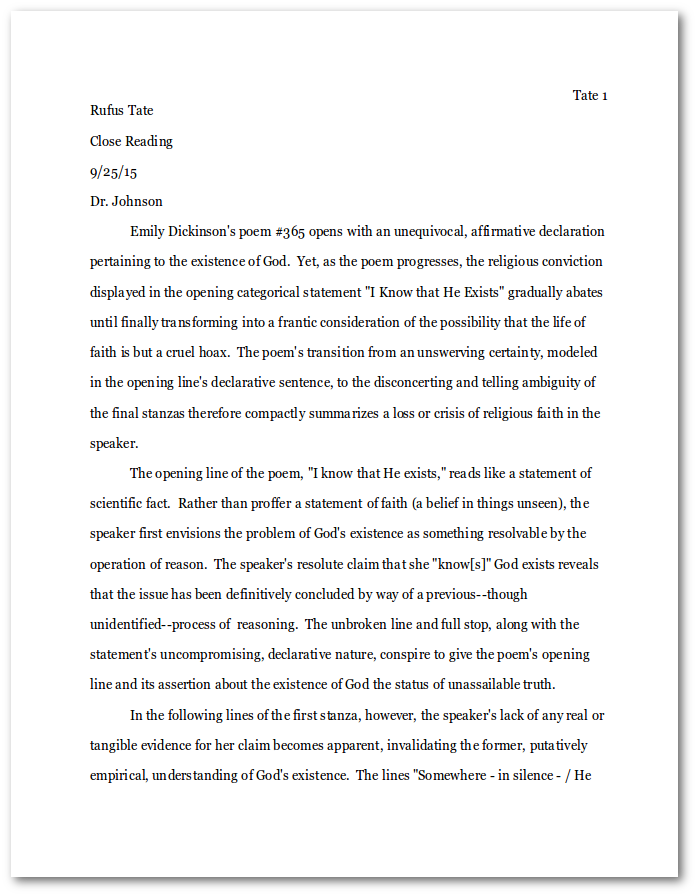
\includegraphics[width=.49\textwidth]{mlastyle}\end{center}
%\end{center}
%\vspace*{\fill}

\newpage
\section{MLA block quote example}
%\vspace*{\fill}
%\begin{center}
%\begin{center}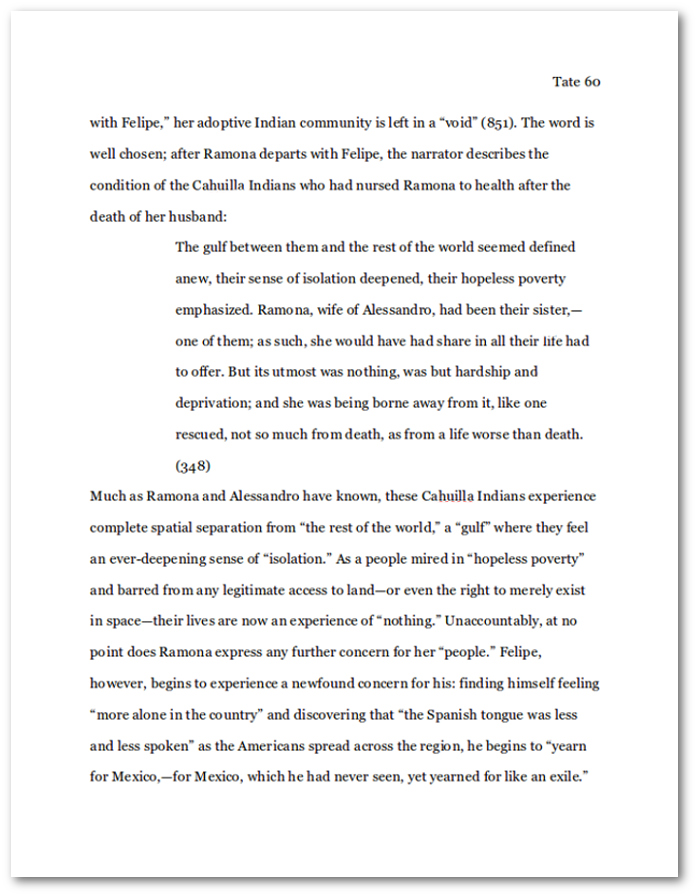
\includegraphics[width=.49\textwidth]{mlablockquote}\end{center}
%\end{center}
%\vspace*{\fill}

\bigskip

\begin{tcolorbox}[enhanced,width=4.2in,left=.35in, right=.35in,
   drop fuzzy shadow southeast,
    boxrule=0.4pt,sharp corners,colframe=black!80!black,colback=white!10]

\medskip

{\scriptsize \begin{flushright} Tate 29 \end{flushright}
\begin{doublespacing}
frequently result in absurdities; an illustration of which may be found in Janie Hinds' 2004 essay on the novel, where she argues the following:
\begin{myenv}The historical Walking Purchase Treaty of 1737, the ‘‘encroachment’’ event alluded to in Edgar Huntly as taking place 30 years before the events of the novel, stipulated that English settlers would own as much territory as they could walk in a day; when the English hired professional runners to cover at least three times as much ground as a person could legitimately cover in walking, the Delaware became understandably hostile, not only about the loss of territory but about the colonists’ trick. (335)\end{myenv}
Hinds here refers to an important moment in the novel when Edgar Huntly explains that the Delaware who formerly lived in the region left due to the “perpetual encroachments of the English colonists” (198). Although Huntly does remark that the departure of the Delaware tribe took place “about thirty years ago,” the event should in no way be confused with the Walking Purchase. Since the novel's setting is almost universally accepted to be in the year 1787, the “encroachments” mentioned by Edgar Huntly must have occurred in, or around, the year 1757—two decades \emph{after} the Walking Purchase. In her attempt to preserve this historical gloss, therefore, Hinds effectively relocates the novel's setting two decades into the past—a claim that contravenes virtually all historical scholarship on the novel and potentially muddles our understanding of the root causes of the native violence in Huntly's narrative. Although the memory of this dishonorable theft of land is undeniably a powerful explanation of the Delaware's revanchist violence within the novel (an argument made by many scholars), we do ourselves a disservice to ignore Brown's plain attempts to have us view his narrative as a statement on “recent incidents.”

\end{doublespacing}}

\bigskip
\smallskip
\smallskip

\end{tcolorbox}



\newpage

\section{In-text citations}
The MLA style uses parenthetical citations to indicate the author and page number of sources. These parenthetical citations take two forms. One form is used when the source you are citing \emph{is named or understood} by your audience. The other form is used when the author being cited is \emph{unknown or unclear}. 

\begin{enumerate}

\item \hloy{Author is named or understood}. \smallskip

In the following sentence the author of the source in question is obvious. Since the author is known to the reader, the parenthetical citation uses \emph{only the page number} of the source: 

\begin{quote}
According to scholar James Frey, "Each American consumes five pounds of ice cream 
annually" (78).
\end{quote}

\item \hloy{Author is not named or understood}. \smallskip

In the following versions of the sentence, however, the author is not stated:

\begin{quote}
According to one scholar, "Each American consumes five pounds of ice cream 
annually" (Frey 78).
\end{quote}

\noindent Or:
\begin{quote}
Studies have shown that the American people consume an average of five pounds of ice 
cream every year (Frey 78).
\end{quote}

\noindent In the first sentence, the author is referred to only as a generic "scholar." To give the reader information on which scholar is being cited, Frey's name is included in the parenthetical citation. In the second sentence the author describes the report, not its author; as a result, the student has included Frey's name to indicate whose report is being referenced. 

\end{enumerate}

\bigskip

\begin{tcolorbox}[colframe=oyster, coltitle=black, sharp corners, title=\ding{52} In-text citations for media like film or music. ]

For media that has a runtime\textemdash like film, television, or music\textemdash MLA now requires that you cite a timestamp within your in-text citations. Use colons to separate hours, minutes, and seconds. For example:

\begin{itemize}
\item According to Rushmore Academy's headmaster, Max is "probably the worst student" at the school (00:04:04-07).

\smallskip

\item In "Don't Hurt Yourself," Beyoncé proclaims "I am the dragon breathing fire" (01:13-15).
\end{itemize}

\end{tcolorbox}



%----DONE-----------

\section{List of Works Cited}

MLA requires a bibliography at the conclusion of the essay that includes the full 
citation of the sources cited within the essay. In MLA, the bibliography is known as the 
\textbf{Works Cited} page. When setting up a Works Cited page, use the following rules and 
characteristics:

\begin{itemize}
\item Center the words "Works Cited" at the top of the page.
\item Use your last name and the page number on the right side of the page's header.
\item Double space the entries.
\item Alphabetize the entries by the author's last name.
\item If an entry runs more than one typed line, indent the second (and any subsequent) line with a 1/2-inch tab.
\item If two or more works by the same author are used, list the entries alphabetically by title. After the first entry, replace the author's name with three dashes followed by a period.
\end{itemize}
\newpage

\section{Works Cited example}
%\begin{center}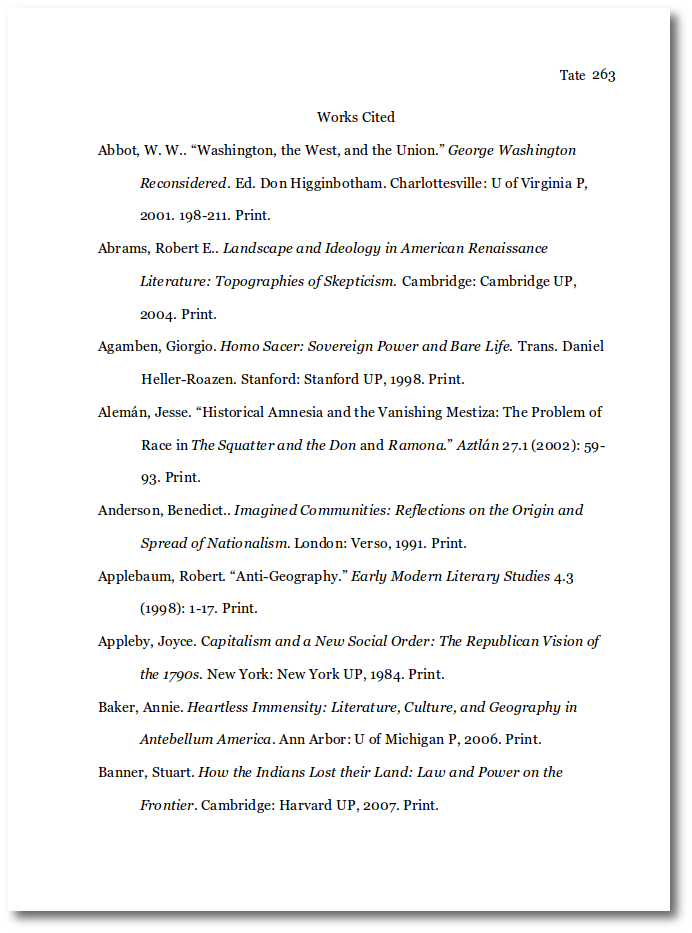
\includegraphics[width=.48\textwidth]{mlaworkscited}\end{center}

\bigskip

\begin{tcolorbox}[enhanced,width=4.2in,left=.3in, right=.3in,
   drop fuzzy shadow southeast,
   halign=flush left,
    boxrule=0.4pt,sharp corners,colframe=black!80!black,colback=white!10]

\medskip

{\scriptsize \begin{flushright} Taylor 12 \end{flushright}

\begin{doublespacing}
\begin{center}Works Cited \end{center}
\hangindent3em{
Abrams, Robert E. \emph{Landscape and Ideology in American Renaissance Literature: Topographies of Skepticism}. Cambridge UP, 2004.}

\hangindent3em{Alemán, Jesse. “Historical Amnesia and the Vanishing Mestiza: The Problem of Race in \emph{The Squatter and the Don} and \emph{Ramona}.” \emph{Aztlán}, vol. 27, no. 1, 2002, pp. 59-93.}

\hangindent3em{Anderson, Benedict. \emph{Imagined Communities: Reflections on the Origin and Spread of Nationalism}. Verso, 1991.}

\hangindent3em{Baas, Robert. “Anti-Geography.” \emph{Early Modern Literary Studies}, vol. 4, no. 3, 1998, pp. 1-17.}

\hangindent3em{Bjorn, Joyce. \emph{Capitalism and a New Social Order: The Republican Vision of the 1790s}. NYU UP, 1984.}

\hangindent3em{Carver, Annie. \emph{Grave Dangers: Spirits and Hauntings in the American Renaissance}. U of Michigan P, 2006.}

\hangindent3em{Graves, Stuart. \emph{How the Indians Lost their Land: Law and Power on the Frontier}. Harvard UP, 2007.}

\hangindent3em{Hill, William. \emph{History of the Blue Ridge}. Dobbs Publishing, 1987.}

\hangindent3em{
- - -. \emph{The Highest Lost Cause: Signal Mountain and the Civil War}. Peach Publishing, 1988.
}

\hangindent3em{
Kleiner, Randy. \emph{Escaping the Redneck Riviera}. Peach Publishing, 1988.
}

\hangindent3em{Linter, Fred. \emph{The Theory of Landscape}. Boston UP, 1999.
}

\hangindent3em{
Zanner, Jeff E. \emph{Language on the Frontier}. Edited by Robert Snooks, Indiana UP, 2012.}

\end{doublespacing}}

\bigskip
\bigskip
\bigskip
\bigskip
\end{tcolorbox}


\newpage

\section{The MLA bibliography}

The eighth edition of the \emph{MLA Handbook}, published in 2016, issued sweeping changes to the formatting of the MLA bibliography. The previous seven editions of the handbook attempted to provide a model citation for every type of source. However, the explosion of internet-based sources and new forms of communication and media made the project of providing guidance on every type of source challenging.  

The new handbook replaces the creation of an ever-growing list of source types with a set of universal guidelines that may be used to formulate a citation for any type of source. These guidelines are referred to as the "core elements."

\section{The MLA core elements}

%\bigskip

%\begin{center}
%\begin{tcolorbox}[colframe=Ahrenge, sharp corners, title=\ding{52} The MLA "core elements"]

%\hangindent1.2cm{
%Author. Title. Title of container (self contained if book), Other contributors (translators or editors), Version (edition), Number (vol. and/or no.), Publisher, Publication Date, Location (pages, paragraphs URL or DOI). 2nd container’s title, Other contributors, Version, Number, Publisher, Publication date, Location, Date of Access (if needed).}

%\end{tcolorbox}
%\end{center}
These core elements are presented in the order they should appear within your bibliography. The proper punctuation that follows each of the core elements is also provided. Thus, you will begin the entry with the author's name, followed by a period. Then the title of the work will be provided, followed by a period. And so on. If one of these core elements does not apply to your source, skip it and move to the next one until you have been through the entire list of elements. The promise of this new approach is that it provides a method for citing any type of source, even those that do not exist yet.

\newpage

\begin{center}
\begin{tcolorbox}[colframe=oyster, coltitle=black, sharp corners, title=\ding{52} The MLA "core elements"]
\begin{itemize} 
{\small
\item Author. 

\item Title. 

\item Title of container (self contained if book), 

\item Other contributors (translators or editors), 

\item Version (edition), 

\item Number (vol. and/or no.), 

\item Publisher, 

\item Publication Date, 

\item Location (pages, paragraphs URL or DOI). 

\smallskip

\rule{8cm}{.1em}

\smallskip

\item 2nd container’s title, 

\item Other contributors, 

\item Version, 

\item Number, 

\item Publisher, 

\item Publication date, 

\item Location, 

\item Date of Access (if needed).
}
\end{itemize}

\end{tcolorbox}
\end{center}


\section{Using the MLA "core elements"}

\subsection{1. Author.}

The first element of a citation is the author's name. Since the MLA bibliography is organized alphabetically by the author's last name, begin your citations with the author's last name, followed by a comma, then the author's first name. If a middle name or initial are supplied, include those after the first name in the entry. Conclude the author element with a period. Often, sources will  have multiple authors. In that case, only the first listed author will use the Last Name, First Name structure. For example: \bigskip

\hangindent1.2cm{
\hl{Taylor, Alan C.} {\emph{A Tour of New Hampshire's Wolf Trees}}. Little and Sons, 1998.
}

\smallskip
 
\hangindent1.2cm{
\hl{Zane, John, Philip Glass and Jane Hinds}. \emph{Recovering the City of Boston}. U of Massachusetts P, 2000.}


\subsection{2. Title of source.}

The title of a source is italicized if it is considered "self-contained" and "independent." Sources that are part of a larger whole, however, are placed in quotation marks. For example, a book is a self-contained and independent source; however, a \emph{chapter in a book} is part of a larger whole. Thus, the title of the book will be italicized while the title of the chapter will appear in quotation marks. Similarly, a television series is an independent whole, so its title will be italicized. However, an episode within the television series is part of the larger program, so its title appears in quotations. For example: \bigskip 

\hangindent1.2cm{
San, Rathanak. \emph{\hl{Escaping Vietnam}}. Peach Publishing, 1988.
}

\smallskip

\hangindent1.2cm{
Taylor, James. "\hl{The Indian Matter of Charles Brockden Brown's Writings.}" \emph{American Literature}, vol. 45, no. 6, 1998, pp. 432-45.} 

\hangindent1.2cm{
"\hl{Say My Name}." \emph{Breaking Bad}, created by Vince Gilligan, performance by Brian Cranston, season 5, episode 7, AMC, 2012.
}

\begin{center}
\begin{tcolorbox}[colframe=oyster, coltitle=black, sharp corners, title=\ding{52} Capitalization of titles in MLA]

MLA has a standardized approach to the capitalization of titles. Regardless of how the title appears on a title page, scholarly journal, or database, use the following information to properly capitalize the title of your source on your Works Cited page:

\medskip
\begin{itemize}
\item Capitalize nouns, pronouns, verbs, adjectives, adverbs, and subordinating conjunctions.

\item Unless they begin the title, do not capitalize articles, prepositions, coordinating conjunctions, or the "to" in infinitive verbs.
\end{itemize}

\end{tcolorbox}
\end{center}


\subsection{3. Title of container,}

Many kinds of sources are smaller parts of larger wholes. MLA refers to these larger wholes as "containers." For example, a chapter is a smaller part of a book. In this sense, the book is the container for the chapter. Similarly, a scholarly article is a smaller part of the scholarly journal that contains it. Newspaper articles, essays in a collection, and television episodes are all contained by a larger context. These containers are italicized in your bibliography. For example, here are the citations for an article in a scholarly journal and a work in a collection of essays:

\bigskip

\hangindent1.2cm{
Taylor, James. "The Indian Matter of Charles Brockden Brown's Writings." \emph{\hl{American Literature}}, vol. 45, no. 6, 1998, pp. 432-45.} \bigskip


\hangindent1.2cm{
Cranston, William. "My Famous Donkey." \emph{\hl{Writings from East Tennessee,}} edited by Jax Ridley, East Tennessee State P, 2011, pp. 77-90.} \bigskip

\noindent Some sources have multiple containers. This is often true for electronic sources. For example, a scholarly article may be contained by both the journal that published it and the academic research database that hosts it online. Consider an article published in the academic database called \href{https://www.jstor.org/}{JSTOR}: \bigskip

\hangindent1.2cm{
Taylor, James. "The Indian Matter of Charles Brockden Brown's Writings." \emph{American Literature}, vol. 45, no. 6, 1998, pp. 432-45. \hl{\emph{JSTOR}, www.jstor.org/stable/8759038475.}} \bigskip

\noindent When citing a source make sure that you represent \emph{every} container so as to truly represent where that source was discovered. 

\subsection{4. Other contributors,}

Your sources will often have a number of other individuals who contributed to the work besides the author(s). You may find sources with one or more of these additional roles:

\begin{itemize}

\item director
\item editor
\item illustrator
\item introducer
\item narrator
\item performer
\item translator
\end{itemize}

\hangindent1.2cm{
Taylor, Alan C. {\emph{A Tour of New Hampshire's Wolf Trees}}. \hl{Edited by Arthur S. Cohen}, Little and Sons, 1998.} \bigskip

\hangindent1.2cm{
Jens, Ryn G. "Morning Glory." \emph{A Runner's Bible,} \hl{translated by Arthur S. Cohen}, Greenwater Press, 1974, pp. 45-58.} \bigskip



\subsection{5. Version,}

Many sources are published in more than one version. The most common version you will encounter in academic research is a new version of a book. Each new version of a book is described as an \textbf{edition}. These versions are numbered in sequential order: 1st edition, 2nd edition, 3rd edition, and so on. There are other kinds of versions, some of which are described below. 

\bigskip 

\hangindent1.2cm{
\emph{The Bible}. \hl{Authorized King James Version}, Oxford UP, 1998.} \bigskip

\hangindent1.2cm{
Smith, John. \emph{Raising Arizona}. \hl{3rd ed.}, Primer Publishing, 1993.} \bigskip

\hangindent1.2cm{
David, Gray. \emph{Blister in the Sun}. \hl{Revised ed.}, Primer Publishing, 1993.} \bigskip

\hangindent1.2cm{
Anderson, Wes. \emph{Rushmore}. 1998. Performance by Bill Murray and Jason Schwartzman, \hl{director's cut}, Buena Vista International, 2017.}\bigskip

\noindent Always ensure that you cite the exact version that you use in your writing. Pagination often differs between editions; versions of a film or other media may vary significantly or have additional content. Failing to cite the specific version of a text will lead to confusion and may make your readers feel that you are sloppy or uncaring. 

\subsection{6. Number,}

Many sources are part of a numbered sequence. For the most part you will encounter this in \textbf{journal articles} and \textbf{books that are part of a numbered series}.
 
\bigskip

\begin{itemize}
\item Journal articles are often collected together in volumes and numbered issues: 
\end{itemize}

\hangindent1.2cm{
Taylor, James. "The Indian Matter of Charles Brockden Brown's Writings." \emph{American Literature}, \hl{vol. 45, no. 6}, 1998, pp. 432-45.}\medskip

\begin{itemize}
\item Some journals do not collect issues into numbered volume numbers; instead, they only publish numbered issues:\end{itemize}

\hangindent1.2cm{
Yeti, Smitty. "Genocide in South America." \emph{Journal of Violence}, \hl{no. 7}, 1990, pp. 221-75.}\medskip

\begin{itemize}
\item When books are too large to be published as a single text, they are organized in volumes: 
\end{itemize}

\hangindent1.2cm{
Smith, Jeb. \emph{A History of American Serial Killers}. \hl{Vol. 6}, Samford UP, 2012.}


\subsection{7. Publisher,}

A publisher is the business or organization responsible for bringing a book, article, website, or other type of source to the public. \textbf{Books} will commonly indicate the publisher on the title or copyright pages, which will be the first few pages of the text: \bigskip 

\hangindent1.2cm{
Lund, Frank. \emph{The Gravest of Errors}. \hl{Indiana UP}, 2012.}\bigskip

\noindent \textbf{Websites} or \textbf{blogs} may not have clear indications for the publisher. However, this information is often included in the footer at the bottom of a homepage or on "About" or "Contact" pages: \medskip

\hangindent1.2cm{
Teeter, Graham. "My Time Alone in Vietnam, a Travel Tale." \emph{Narratives from the Edge}, \hl{Society of World Geographers}, www.edgenarratives.com/teeter}. \bigskip

\noindent Television series and films are often created by a large array of producers and companies. However, cite only the organization that had the primary responsibility for production:\bigskip 

\hangindent1.2cm{
Anderson, Wes. \emph{Rushmore}. Performance by Bill Murray and Jason Schwartzman, \hl{Buena Vista International}, 1998.}\bigskip



\begin{center}
\begin{tcolorbox}[colframe=oyster, coltitle=black, sharp corners, title=\ding{52} When \emph{not} to include the publisher]
The MLA stylebook explains several situations where a publisher's name is \emph{not} required in the citation: 

\begin{itemize}
\item A periodical (academic journal, newspaper, magazine, etc.)
\item A work published by its author.
\item A website whose title is essentially the name of the publisher.
\item A website that does not help produce the source, only host it (academic database, YouTube, etc.)
\end{itemize}

\medskip

Be careful, however, to include things like the electronic database name or platforms like YouTube as \textbf{containers}, described above.


\end{tcolorbox}
\end{center}




\subsection{8. Publication date,}

Most sources appropriate for academic research will clearly disclose the date, or dates, of publication. This information will often appear in the front matter of books or journals, or in the masthead of newspapers. 

Online sources, however, present a problem. Sometimes it is unclear when an online source was published. Other times the online source may be a digital version of a print source which may have been published at a different time. 

When a source has more than one publication date, cite only the version that you are using in your own writing. For example, if you are citing a newspaper article you read online, you should cite the date disclosed on the online version, not the corresponding print version. Failing to do this may cause problems if the online version was edited after the newspaper went to print.

\subsection{9. Location,}

The location of a source largely refers to a source's \textbf{page number, or numbers}. However, many types of sources do not have page numbers. A web page's location, for example, is a \textbf{URL}. And a painting or statue's location would be the \textbf{physical location} of the museum where you viewed it in person. 

\begin{itemize}
\item A chapter in a book:
\end{itemize}

\hangindent1.2cm{
Tate, Justin. "Ordering Wine in Paris." \emph{An American's Guide to French Cuisine}, U of Tennessee P, 1989, \hl{pp. 45-61}}. \bigskip

\noindent If the source is only on a single page, use p. rather than pp. to indicate the page number.

\begin{itemize}
\item A website:
\end{itemize}

\hangindent1.2cm{
Grisham, Wyatt. "A Soccer Mom's Lament." \emph{Sports and Parenting}, 28 Oct. 2017, \hl{www.sandp.org/soccermomslament}}. \bigskip

\noindent URLs can be challenging to present because of their length or mutable nature. If possible, use what is known as a permalink\textemdash a permanent URL associated with online content. These permalinks will not change over time. You may also find online content with a DOI, a digital object identifier. You may cite this DOI in place of a URL. If a URL is too long to include in your bibliography, you may use a shortened version of the URL by citing the domain name of the source. For example: www.nytimes.com.


\begin{center}
\begin{tcolorbox}[colframe=oyster, coltitle=black, sharp corners, title=\ding{52} Note]

Previous versions of the MLA handbook required that the city of publication be included for the citation of books. This is no longer required. 


\end{tcolorbox}
\end{center}




\begin{itemize}
\item A material object or work of art:
\end{itemize}

\hangindent1.2cm{
Wayins, Brill. \emph{Lone Pine Tree}. 2001, \hl{Hood Museum of Art, Hanover}.

\section{The MLA bibliography}

While the new edition of the MLA Handbook largely dispenses with specific templates for making citations, I have retained the following examples for this edition of the \emph{Open Handbook}. Although the objective of the MLA "core elements" is to dispense totally with standardized templates, I find that these examples are still a helpful guide, especially for students who lack experience with this style of citation. 

The following section provides examples for citing sources that are commonly found in academic writing. The various forms have been organized into sections on \textbf{books}, \textbf{periodicals}, \textbf{electronic sources}, and \textbf{other types of sources} that are less common.


\section{Book forms}

\subsection{A book by one author}

\hangindent1.2cm{
Taylor, Herman. {\emph{A Tale of One City}}. Little and Sons, 1998.
}


\subsection{Two or more works by the same author(s)}

\hangindent1.2cm{
San, Rathanak. \emph{Escaping Vietnam}. Peach Publishing, 1988.}

\medskip

\hangindent1.2cm{
\noindent- - -. \emph{The Golden Triangle}. Gray and Long, 1999.}

\medskip

\begin{itemize}\item If you cite two works by the same author, use the author's first and last name in the first instance. Use three dashes followed by a period in place of the author's name for any additional works. Place the works in alphabetical order using the first important word in the title.\end{itemize}

\subsection{Two or three authors}


\hangindent1cm{
Roberts, John, Philip Glass and Jane Hinds. \emph{Recovering the City of Boston}. U of Massachusetts P, 2000.}

\begin{itemize}\item Cite the first author using the typical Last Name, First Name format. For each subsequent author, use First Name Last Name.\end{itemize}

\subsection{Four or more authors}


\hangindent1.2cm{
Bankston, Jonathan, et al. \emph{On Barns}. Woodcraft Publishing, 2013.}

\begin{itemize}\item If a work has four or more authors, you may give the first author's name and replace the other authors with the Latin term "et al," which means "and others." \end{itemize}

\subsection{A book with an editor}
\hangindent1.2cm{
James, Henry. \emph{Portrait of a Lady}. Edited by Leon Edel, Houghton, 1963.}

\begin{itemize}\item If a work has multiple editors, use "Editors" followed by the editors' names in the order they are listed in the source. \end{itemize}


\subsection{An edition (other than the first)}
\hangindent1.2cm{
Thompson, Fred. \emph{Why I Fight}. 3rd ed., Vanity Publications, 2000.}

\subsection{A republished book}

\hangindent1.2cm{
James, Esther. \emph{My Life}. 1946. Random House, 2001.}

\begin{itemize}\item A republished book is one that was previously published in a different form, perhaps even from a different publisher. For books of this kind, indicate the original year of publication after the title. \end{itemize}

\subsection{Corporate author (written by organization or government)}


\hangindent1.2cm{
John Bigam Society. \emph{The Religions of Kenya}. Nairobi Publishing, 2000.}

\medskip 

\hangindent1.2cm{
\noindent United States, Department of Transportation. \emph{State Highway Signage Regulations}. Government Publishing Office, 2002.}

\begin{itemize}\item If the author of a work is a government or institution, use the name of that organization in place of the author. If the text is the publication of a government, include the name of the department or agency. \end{itemize}

\subsection{An anthology}
\hangindent1.2cm{
Foner, Eric, editor. \emph{An American Voice: A Collection of America's Finest} \emph{Essays}. McKinley and Smith, 2011.}

\subsection{Work in an anthology or collection of essays}
\hangindent1.2cm{
Graves, Thomas. "The History of our National Anthem." \emph{An American Voice: A Collection of America's Finest Essays,} edited by Eric Foner, McKinley and Smith, 2011, pp. 20-41.}

\subsection{No author or editor}

\hangindent1.2cm{
\emph{A Guide to Boston}. Beantown Publishing, 2000.}

\subsection{Forward, introduction, preface, or afterward}

\hangindent1.2cm
{Knox, John. Introduction. \emph{The Life of James}, by Elders Johnson, Random House, 2009, pp. 1-8.}



\subsection{A book with a translator} 
\hangindent1.2cm{
McDougle, Astrid. \emph{The Basics of Gaelic}. Translated by Paddy Maloney, Vintage, 1990.}

\subsection{Multivolume work}

\hangindent1.2cm{Graves, Johanna. \emph{Ronald Reagan and the Iran-Contra Affair}. Vol. 7, Greenstalk Publishers, 1988.}

\subsection{Book in a series}


\hangindent1.2cm{
Smith, Rod. \emph{American Economic Expansion in the Nineteenth Century}. Edited by Andrew Stills, Alfred A. Knopf, 1988. History of American Economic Development.}

\begin{itemize}\item Occasionally, a press will publish a series of books about a single topic. If your source is a book in a published series, indicate the name of the series at the conclusion of the citation. \end{itemize}

\subsection{Dictionary or encyclopedia entry}

\hangindent1.2cm{
"Suzerian." \emph{Merriam-Webster's Collegiate Dictionary}. 10th ed., 2008.}

\begin{itemize}\item If you are citing an entry from a reference text like a dictionary or encyclopedia that is organized alphabetically, you do not need to indicate the page number.\end{itemize}

\subsection{Sacred text}

\hangindent1.2cm{
\emph{The Bible}. \hl{Authorized King James Version}, Oxford UP, 1998.} \bigskip

\begin{itemize}\item If you are citing a particular edition of a sacred text, such as the Bible, Koran, or Torah, include that information.\end{itemize}


\subsection{Book with title within the title}


\hangindent1.2cm{
Hixson, Fred. \emph{On Cormac McCarthy's }Blood Meridian. Plainspeak P, 2000.}

\begin{itemize}\item If a book title contains the title of another book or article, remove the italics to indicate the title
of the other work.\end{itemize}
%--------------------------------------------------------------------------------------------
%Periodicals
%-------------------------------------------------------------------------------------------


\section{Periodical forms}

\subsection{Article in a scholarly journal with volume and issue numbers}
\hangindent1.2cm{
Taylor, James. "The Indian Matter of Charles Brockden Brown's \emph{Edgar Huntly}." \emph{American Literature}, vol. 45, no. 6, 1998, pp. 432-45.}

\subsection{Article in a scholarly journal that only numbers issues}
\hangindent1.2cm{
Johnston, Johanna. "A Reading of \emph{Moby Dick}." \emph{North Dakota Quarterly}, no. 45, 1978, pp. 45-56.}


\subsection{Article with a title in the title}
\hangindent1.2cm{
Glastonbery, Wes. "On Teaching \emph{Blood Meridian}." \emph{The Journal of College Writing}, vol. 4, no. 5, 2011.}

\begin{itemize}\item If an article's title contains the title of another text, add italics to internal title.\end{itemize}

\subsection{Article in a newspaper}
\hangindent1.2cm{
McKinley, Robert. "Cat Saved from Dog." \emph{The New York Times}, 7 Oct. 2011, p. B2.}

\begin{itemize}\item When an article appears on nonconsecutive pages, indicate the page where article begins 
then use a "+" sign. \end{itemize}

\subsection{Letter to the editor of a newspaper}
\hangindent1.2cm{
Johnson, Smitty. "Reduce our Property Taxes." Letter, \emph{Henniker Telegraph}, 14 Oct. 2013, p. A2} 

\subsection{A review}
\hangindent1.2cm{
Smith, James. Review of \emph{The Orchard Revival}, by Cormac Freedman. \emph{Oregon Magazine}, 23 Oct. 2011, pp. 34-36.} 

\begin{itemize}
\item If the review has a title, include it in quotations after the author's name.
\end{itemize}

\subsection{An unsigned article in a newspaper}
\hangindent1.2cm{
"A Walk Down Nostalgia Lane." \emph{Chicago Sun}, 28 Oct. 2013, p. B6.}

\subsection{Article in a magazine}
\hangindent1.2cm{
Smith, Jim. "Remembering Tony." \emph{The New Yorker}, Jan. 2010, pp. 12-18.}


%--------------------------------------------------------------------
\section{Online sources}

\begin{center}
\begin{tcolorbox}[colframe=oyster, coltitle=black, sharp corners, title=\ding{52} URLs \& DOIs]

Include the address of any content that you find online.\smallskip

\begin{itemize}
\item When possible, use a "stable url" or "permalink" for this purpose. This address will never change and will allow others to find the content easily. 

\item Some online sources have what is known as a Digital Object Identifier, or DOI. If the source has a DOI, use it in place of a URL.

\item When using a URL, remove the "http://" or "https://" that precedes the address. Instead, begin your url with "www."

\item If a URL is too long to include in your bibliography, you may use a shortened version of the url by citing the domain name of the source. For example: www.nytimes.com.
\end{itemize}

\end{tcolorbox}
\end{center}

\subsection{Article in an online database}

\hangindent1.2cm{
Taylor, Abel. "\emph{Moby Dick} and the Cold War." \emph{American Literature}, vol. 45, no. 6, 2010, pp. 45-57. \emph{JSTOR}, www.jstor.org/stable/ 785463258.}

\begin{itemize}\item Cite the source as you would a print article then include the database name, stable url, or DOI (Digital Object Identifier). \end{itemize}

\subsection{A website as a whole} 
\hangindent1.2cm{
Zimmerman, Constantine. \emph{The Moose Report}. New Hampshire Hiking Club, www.moosereport.org.}


\subsection{A work from a website}
\hangindent1.2cm{
Reagan, John. "The Judo Champion Parent." \emph{Parenthood Online}. 11 Oct. 2011, www.parenthoodonline.org/judo.}


\subsection{Article in an online scholarly journal}
\hangindent1.2cm{
Nelson, Grady. "Electronic Literature Comes of Age." \emph{e-Lit Quarterly}, no. 2, 2012, pp. 45-60. www.elit.org/2/2012/grady.pdf.}

\subsection{Article in an online newspaper}
\hangindent1.2cm{
Taylor, Robert C. "Harvesting Undersea Sponges." \emph{New York Times}, 23 Nov. 2000, www.nytimes.com/2000/11/23/us/sponges.}


\subsection{Article in an online magazine}
\hangindent1.2cm{
James, Brian Taylor. "The New War on Terror." \emph{Foreign Affairs Monthly}, Errata Publishing, 2 Oct. 2009, www.famonthly.org /2009/10/james-terror.}



%Online editorial
%Online film review

\subsection{Email}

\hangindent1.2cm{
Cooledge, John. "My Election Thoughts." Received by Mel Smith, 12 Nov. 2012.}

\begin{itemize}
\item For an email message, use the subject line of the email as the title. Indicate the person, or persons, who received the email after the title and the date it was sent.
\end{itemize}


%Posting from an online discussion board

\subsection{Article from an online reference work, such as Wikipedia}
\hangindent1.2cm{
"Al-Qaeda." \emph{Wikipedia}. Wikimedia Foundation, 25 Aug. 2017, https://en.wikipedia.org/wiki/Al-Qaeda.}



\subsection{Podcast:}
\hangindent1.2cm{
Zeender, Nathan, James Spenser, and Michael Tonsmeire. "Dark Lagers." \emph{Basic Brewing Radio}, 31 Jan. 2013, http://traffic. libsyn.com/basicbrewing/bbr01-31-13darklagers.mp3.}

\section{Other types of sources}

\subsection{A dissertation}
\hangindent1.2cm{
Redburn, Marcus. "A Study of Melville's Aesthetics." Dissertation, Boston University, 1978.}

\subsection{Artwork}
\hangindent1.2cm{
Freeman, Dianna. \emph{Still Life 7}. 2009, Hunter Museum of Art, Chattanooga.}

\begin{itemize}\item For a work of art with no title, include a description of the medium after the author's name. For example: photograph, oil on canvas, watercolor, mixed media. \end{itemize}

\subsection{Film or video clip}
\hangindent1.2cm{
Anderson, Wes, director. \emph{Rushmore}. Buena Vista International, 1998.}\bigskip

\noindent Anderson, Wes, director. \emph{Rushmore}. Performance by Bill Murray, Buena Vista International, 1998.}\bigskip

\begin{itemize}\item If the focus of your writing is on a particular performer rather than the film as a whole, include the lead performers in the film after the director. \end{itemize}


%Broadcast interview
%Published interview
%Unpublished letter
%Published letter
%Map or chart
%Musical score
%Sound recording
%Oral presentation
%Paper from a conference
%Performance
%Television or radio program
%Pamphlet, brochure, or press release
%Legal source
%A digital file, such as .mp3, .pdf, etc.

%----------------------------------------------------------------------------------------
% END OF SECTION
%----------------------------------------------------------------------------------------
%---------------------------------------------------------------------------------------- % THE CHICAGO STYLE  %----------------------------------------------------------------------------------------

\chapter{Chicago style}

\section{Formatting the Chicago essay}

When setting up your word processor for a Chicago-formatted document, use the
following settings and rules:

\begin{itemize} 

\item Use one-inch margins on all sides of the document. 

\item Place the page number on the right side of each page in the
document's header. If instructed to do so by a professor, include your last name before the page number on each page. 

\item Double space the document. 

\item Block quotes are formed when a quote runs more than 100 words. Indent the entire  block of text
with a 1/2-inch tab from the left margin. 
\item Endnotes and bibliographic entries are single-spaced with a blank line separating them. 
\item Indent the first line of a note entry with a 1/2-inch tab. 
\item Indent the second, and any subsequent, line of a bibliographic entry with a 1/2-inch tab. 
\item The Chicago form requires a title page. The title of the essay is centered about  1/3 down
the top of the page. Place your name, course information, and date on three
separate, centered lines at the center of the document.
\end{itemize}
\bigskip

\begin{center}
\begin{tcolorbox}[colframe=oyster, coltitle=black, sharp corners, title=\ding{52} Note!]
The title page is \emph{counted but not
numbered}. Therefore,  begin your essay with page 2.
\end{tcolorbox}
\end{center}

\section{A model of the Chicago essay} \newpage 

%\begin{center}
%
\includegraphics[width=.50\textwidth]{chicagotitle} \end{center}

\begin{tcolorbox}[enhanced,width=4.2in,left=.3in, right=.3in,
   drop fuzzy shadow southeast,
    boxrule=0.4pt,sharp corners,colframe=black!80!black,colback=white!10]

{\scriptsize 

\vspace{3.5cm}

\begin{center}Emily Dickenson's Poem \#365: "I know that He exists"
\vspace{3cm}

Rufus Tate

\vspace{5cm}
Writing 002

Dr. Clem Spanning

October 28, \the\year \end{center}

}

\vspace{.55cm}
\end{tcolorbox}

\newpage

%\begin{center} 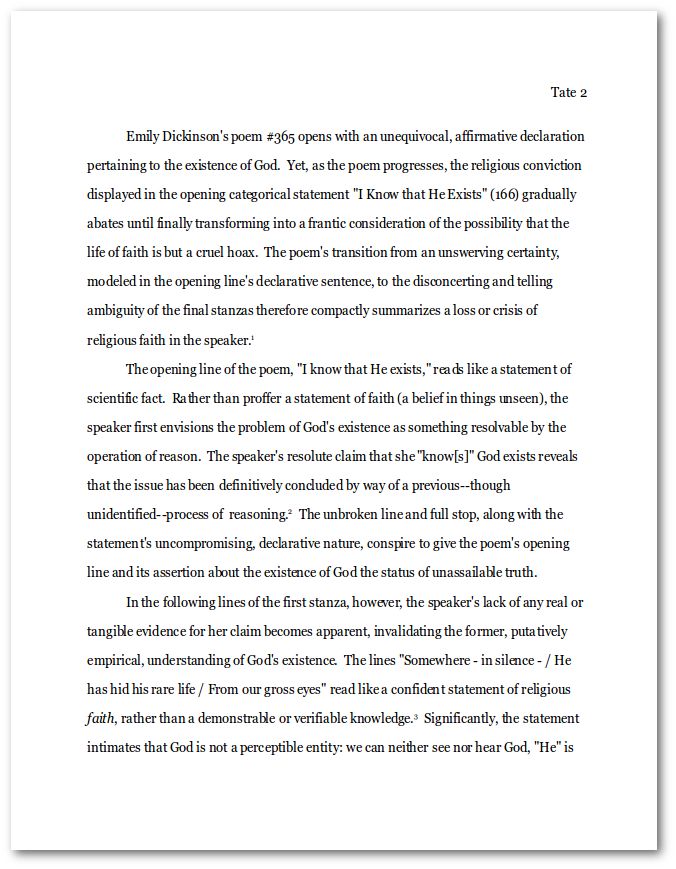
\includegraphics[width=.50\textwidth]{chicago2} \end{center}

\bigskip

\begin{tcolorbox}[enhanced,width=4.2in,left=.3in, right=.3in,
   drop fuzzy shadow southeast,
    boxrule=0.4pt,sharp corners,colframe=black!80!black,colback=white!10]

\medskip

{\scriptsize \begin{flushright} Tate 2 \end{flushright}
\begin{doublespacing}


\hspace{1.4em} Emily Dickinson's poem \#365 opens with an unequivocal, affirmative declaration pertaining to the existence of God.  Yet, as the poem progresses, the religious conviction displayed in the opening categorical statement "I Know that He Exists" gradually abates until finally transforming into a frantic consideration of the possibility that the life of faith is but a cruel hoax.  The poem's transition from an unswerving certainty, modeled in the opening line's declarative sentence, to the disconcerting and telling ambiguity of the final stanzas therefore compactly summarizes a loss or crisis of religious faith in the speaker.\textsuperscript{1}  
  
\hspace{1.4em} The opening line of the poem, "I know that He exists," reads like a statement of scientific fact.  Rather than proffer a statement of faith (a belief in things unseen), the speaker first envisions the problem of God's existence as something resolvable by the operation of reason.  The speaker's resolute claim that she "know[s]" God exists reveals that the issue has been definitively concluded by way of a previous--though unidentified--process of  reasoning.  The unbroken line and full stop, along with the statement's uncompromising, declarative nature, conspire to give the poem's opening line and its assertion about the existence of God the status of unassailable truth.  

\hspace{1.4em}In the following lines of the first stanza, however, the speaker's lack of any real or tangible evidence for her claim becomes apparent, invalidating the former, putatively empirical, understanding of God's existence. The lines "Somewhere - in silence - / He has hid his rare life / From our gross eyes" read like a confident statement of religious faith, rather than a demonstrable or verifiable knowledge.\textsuperscript{2}  Significantly, the statement intimates that God is not a perceptible entity: we can neither see nor hear God, "He" is both hidden "Somewhere - in Silence" and away "From our gross eyes." 


\end{doublespacing}}
\vspace{.33in}


\end{tcolorbox}

\section {In-text citations}

In the Chicago form, an in-text citation is indicated by a superscript number
resembling the following:

\begin{quote} Recent scholarship on the concept of sovereignty has displayed a
remarkable lack of interest in the role of private property.\textsuperscript{7}
\end{quote}

\noindent This in-text reference will correspond to a citation on the Notes page
at the conclusion of the document, such as this one:

\begin{singlespace}
\begin{quote} \hspace{.4in}7. Giorgio Agamben, \emph{Homo Sacer: Sovereign Power
and Bare Life} (Stanford: Stanford University Press, 1998), 96. \end{quote}
\end{singlespace}

\section{The Notes page}

In the Chicago style, the endnotes appear on what is known as the \textbf{Notes}
page\textemdash a separate page that directly follows the conclusion of the
essay. The Notes page is organized as a numbered list that presents each
citation in the order that it appears within the essay. Thus, your first
citation will be note 1, your second will be note 2, and so on.

\section{Setting up the Notes page} When setting up the Notes page, use the
following rules:

\begin{itemize} \item Center the word "Notes" at the top of the page. \item
Single-space the endnotes with a line separating entries. \item Indent the first
line of an endnote entry with a 1/2-inch tab. \end{itemize}

\newpage
\section{Example Chicago Notes page} 

\begin{tcolorbox}[enhanced,width=4.2in,left=.3in, right=.3in,
   drop fuzzy shadow southeast,
    boxrule=0.4pt,sharp corners,colframe=black!80!black,colback=white!10]

\medskip

{\scriptsize \begin{flushright} Tate 12 \end{flushright}
\begin{singlespacing}

\begin{center} Notes \end{center}

\hspace{2em}1. Lance Carter, \emph{On Building Copper Stills} (New York: Random House, 1988), 10.\\

\hspace{2em}2. Ibid., 20.\\

\hspace{2em}3. George Crary, \emph{The Silence of Pigs} (1879; reprint, New York: Faber Books, 2010), 100.\\

\hspace{2em}4. Ibid.\\

\hspace{2em}5. Ibid.\\

\hspace{2em}6. Ibid., 2.\\

\hspace{2em}7. Ibid., 22.\\

\hspace{2em}8. Ibid., 7.\\ 

\hspace{2em}9. Jonas Whale, "The Southern Mystique," in \emph{Faulkner's Mississippi Drinkers}, ed. Gray Davis (Chattanooga: University of Tennessee Press, 2000), 99.\\

\hspace{2em}10. Ibid., 8.\\

\hspace{2em}11. Crary, \emph{Silence}, 45.\\

\hspace{2em}12. Jedediah Cross, \emph{Woods, Bear, and Corn} (Danville: White Lightning Books, 1988), 12.\\

\hspace{2em}13. Crary, \emph{Silence}, 45.\\

\hspace{2em}14. Ibid.\\

\hspace{2em}15. Rufus Tate, \emph{Lipstick on a Pig} (New York: Goose Pimple Press, 1988), 70.\\

\hspace{2em}16. Ibid., 31.\\

\hspace{2em}17. William T. Bibble, "Farming Your Way to Millions," \emph{Alabama Agriculture} 4, no. 8 (1979): 20.\\


\end{singlespacing}
}
\bigskip


\end{tcolorbox}

\newpage

\section{Rules for making the notes} The Chicago form uses an economical
practice that reduces the  work involved in presenting the essay's footnotes or
endnotes. While this design  ultimately means less typing, a number of strict
rules must be followed:

\begin{itemize} \item Present the citations in the numerical order as they
appear within the text.

\item The first time a source is cited, use the \emph{full} Chicago notes form.

\item If the same source is used more than once, the \emph{shorthand} version of
the Chicago  notes form is used the second (and each subsequent) time. The
shorthand version  contains \textbf{a)} the author's last name, \textbf{b)} a
shortened version of the title,  and \textbf{c)} the page number(s) of the
citation.

\item If a single source is used twice or more in a row, the Latin abbreviation
"Ibid." is  used along with the page number, rather than the shorthand version
of the form.  (Ibid. means "in the same place.")

\item If the same source is used \emph{twice in a row} and the citation \emph{is
from  the same page as the previous citation}, "Ibid." is used by itself without
the  page number.  \end{itemize}

\section{The Bibliography page} The Chicago style also requires that you include
a bibliography page at the conclusion of your essay. As you will see in the next
section, the bibliography  form differs slightly from the notes form, so take
care to use the correct one. To format the bibliography page, use the following
rules:

\begin{itemize} \item Place the bibliography page after the notes page. \item
Center the word "Bibliography" at the top of the page. \item Single-space
entries with a line separating entries. \item Alphabetize by the author's last
name. \item Indent the second (and any subsequent) line of an entry with a
1/2-inch tab. \end{itemize}

\newpage \section{Example Chicago Bibliography page} 
\begin{tcolorbox}[enhanced,width=4.2in,left=.3in, right=.3in,
   drop fuzzy shadow southeast,
    boxrule=0.4pt,sharp corners,colframe=black!80!black,colback=white!10]

\medskip

{\scriptsize \begin{flushright} Tate 12 \end{flushright}
\begin{singlespacing}

\begin{center}Bibliography \end{center}

\hangindent2em{Allen, Tate. \emph{White Lightning}. Edited by Leon Edel. Boston: Houghton, 1963.}\\

\hangindent2em{Fulton, Fendal. \emph{Bootleggers and the Birth of NASCAR}. Legrange: Automotive Books, 1974.}\\

\hangindent3em{Graves, Thomas. "Building a Copper Worm." In \emph{An American Art: Illegal Moonshine and the Foxfire Tradition}, edited by Eric Foner, 77-88. Atlanta: McKinley and Smith, 2011.}\\

\hangindent3em{Knox, John. Introduction to \emph{The Life of Popcorn Sutton}, by Elders Johnson, 2-9. New York: Random House, 2009.}\\

\hangindent3em{Linter, Jerry S. Review of \emph{The Orchard Revival}, by Cormac Freedman. \emph{Tennessee
Literary Review} 120, no. 4 (1998): 20-23.}\\

\hangindent3em{Mellon, Batson. \emph{A History of the Tennessee Valley: 1780-1980}. Baltimore: Brown Bag Press, 1998.}\\

\hangindent3em{Robers, John, Philip Glass and Jane Hinds. \emph{Mason Jars and Corn Whiskey}. Boston: University of Tennessee Press, 2000.}\\

\hangindent3em{Talmage, Lance. \emph{Copper Stills in Appalachia}. New York: Random House, 1988.}\\

\hangindent3em{Zeb, Fred and Linda Tanner, eds. \emph{Anarchy on the River's Edge}. Chattanooga: Lookout Publishing, 1974.}\\

\hangindent3em{Zoltan, Hayden. "Southern Tradition as Politics." \emph{American Folkways} 45, no. 6 (2010): 45-61. doi: 12.2398/ahl.483.1.112.}\\


\end{singlespacing}}
\vspace{3.2cm}

\end{tcolorbox}

\newpage

\section{The Chicago Bibliography}

The following section provides examples for citing sources that are commonly
found in academic writing. The various forms have been organized into sections 
on \textbf{books}, \textbf{periodicals}, \textbf{electronic sources}, and
\textbf{other types of sources} that are less common.

\begin{itemize}
\item In each form, the first citation is the \textbf{bibliography} form and the
second citation is the \textbf{notes} form.
\end{itemize}

\section{Book forms}

\subsection{A book by one author}


\begin{center}{Bibliography}\end{center}

\begin{singlespace}
\noindent\hangindent1.2cm {Taylor, Herman. \emph{A Tale of One City}. New York:
Little and Sons, 1998.}
\end{singlespace}




\begin{center}{Notes}\end{center} 
\begin{singlespace}
\noindent\hspace{1.2cm}1. Herman Taylor,
\emph{A Tale of One City} (New York: Little and Sons, 1998), 77.
\end{singlespace}


\subsection{Multiple authors}


\begin{center}{Bibliography}\end{center}

\begin{singlespace}
\noindent\hangindent1.2cm{Roberts, John, Philip Glass and Jane Hinds.
\emph{Recovering the City of Boston}. Boston: University of Massachusetts Press,
2000.}
\end{singlespace}


\begin{center}{Notes}\end{center}
\begin{singlespace}
\noindent\hspace{1.2cm}1. John Roberts, Philip Glass and Jane Hinds,
\emph{Recovering the City} \emph{of Boston} (Boston: University of Massachusetts
Press, 2000), 77.
\end{singlespace}



\begin{itemize} \item Include up to three authors in the \textbf{notes} form.
\item If there are four or more, give the first author's name and then use "et.
al." ("and others") to replace the other authors.  \item In the
\textbf{bibliography} form, include up to ten authors. If there are more than
ten authors, give the first seven and then use "et. al." \end{itemize}

\subsection{A book with an editor}

    
\begin{center}{Bibliography}\end{center}
\begin{singlespace}
\noindent\hangindent1.2cm{James, Henry. \emph{Portrait of a Lady}. Edited by
Leon Edel. Boston: Houghton, 1963.}
\end{singlespace}

\begin{center}{Notes}\end{center}
\begin{singlespace}
\noindent\hspace{1.2cm}12. Henry James, \emph{Portrait of a Lady}, ed. Leon Edel
(Boston: Houghton, 1963), 77.
\end{singlespace}


\subsection{Book with editor only}

\begin{center}{Bibliography}\end{center}
\begin{singlespace}
\noindent\hangindent1.2cm{Smith, Edward, ed. \emph{Stuck in Goshen}. Nashville:
Greenwood Press, 1963.}\\

\noindent\hangindent1.2cm{Zebe, Fred and Linda Tanner, eds. \emph{Anarchy on the
River's Edge}. Chattanooga: Lookout Publishing, 1974.}
\end{singlespace}

\begin{center}{Notes}\end{center}
\begin{singlespace}
\hspace{1.2cm}17. Edward Smith, ed., \emph{Stuck in Goshen} (Nashville:
Greenwood Press, 1963), 77.\\

\noindent\hspace{1.2cm}18. Fred Zebe and Linda Tanner, eds., \emph{Anarchy on the River's
Edge}. (Chattanooga: Lookout Publishing, 1974), 77.
\end{singlespace}

\begin{itemize} \item If there are multiple editors, use "eds." \end{itemize}

\subsection{An edition (other than the first)}
\begin{center}{Bibliography}\end{center}

\begin{singlespace}
\noindent\hangindent1.2cm{Thompson, Fred. \emph{Why I Fight}. 3rd ed. New York:
Vanity Publications, 2000.}
\end{singlespace}

\begin{center}{Notes}\end{center}

\begin{singlespace}
\noindent\hspace{1.2cm}12. Fred Thompson, \emph{Why I Fight}, 3rd. ed. (New
York: Vanity Publications, 2000), 77.
\end{singlespace}

\subsection{Corporate author (written by organization or government)}

\begin{singlespace}
\begin{center}{Bibliography}\end{center} \noindent\hangindent1.2cm{John Bigan
Society. \emph{The Religions of Kenya}. New York: John Bigan Publishing, 2000.}
\end{singlespace}

\begin{center}{Notes}\end{center} 
\begin{singlespace}
\noindent\hspace{1.2cm}10. John Bigan Society,
\emph{The Religions of Kenya} (New York: John Bigan Publishing, 2000), 77.
\end{singlespace}

\subsection{An anthology} \begin{center}{Bibliography}\end{center}

\begin{singlespace}
\noindent\hangindent1.2cm{Foner, Eric, ed. \emph{An American Voice: A Collection
of America's Finest Essays}. Boston: McKinley and Smith, 2011.}
\end{singlespace}

\begin{center}{Notes}\end{center} 

\begin{singlespace}
\noindent\hspace{1.2cm}15. Eric Foner, ed.,
\emph{An American Voice: A Collection of America's Finest Essays} (Boston:
McKinley and Smith, 2011), 77.
\end{singlespace}


\subsection{Work in an anthology}

\begin{singlespace}
\begin{center}{Bibliography}\end{center} \noindent\hangindent1.2cm{Graves,
Thomas. "The History of our National Anthem." In \emph{An American Voice: A
Collection of America's Finest Essays}, edited by Eric Foner, 77-88. Boston:
McKinley and Smith, 2011.}
\end{singlespace}


\begin{center}{Notes}\end{center} 

\begin{singlespace}
\noindent\hspace{1.2cm}13. Thomas Graves, "The
History of our National Anthem," in \emph{An American Voice: A Collection of
America's Finest Essays}, ed. Eric Foner (Boston: McKinley and Smith, 2011),
77-88.
\end{singlespace}
\subsection{No author or editor}

\begin{center}{Bibliography}\end{center}

\begin{singlespace}
\noindent\hangindent1.2cm{\emph{A Wicked Guide to Boston}. Boston: Beantown
Publishing, 2000.}
\end{singlespace}


\begin{center}{Notes}\end{center} 
\begin{singlespace}
\noindent\hspace{1.2cm}25. \emph{A Wicked Guide to Boston} (Boston: Beantown Publishing, 2000), 22.
\end{singlespace}


\subsection{Introduction, preface, forward or afterward}
\begin{center}{Bibliography}\end{center} 

\begin{singlespace}
\noindent\hangindent1.2cm{Knox, John.
Introduction to \emph{The Life of James}, by Elders Johnson, 2-9. New York:
Random House, 2009.}
\end{singlespace}


\begin{center}{Notes}\end{center} 
\begin{singlespace}
\noindent\hspace{1.2cm}33. John Knox,
introduction to \emph{The Life of James}, by Elders Johnson (New York: Random
House, 2009), 7.
\end{singlespace}


\begin{itemize}\item Substitute the word introduction with preface, afterward,
or foreward as needed.\end{itemize}

\subsection{Book with a translator}

\begin{center}{Bibliography}\end{center} 

\begin{singlespace}
\noindent\hangindent1.2cm{McDougle,
Astrid. \emph{The Basics of Gaelic}. Translated by Paddy Maloney. New York:
Vintage, 1990.}
\end{singlespace}

\begin{center}{Notes}\end{center} 

\begin{singlespace}
\noindent\hspace{1.2cm}45. Astrid McDougle,
\emph{The Basics of Gaelic}, trans. Paddy Maloney (New York: Vintage, 1990), 22.
\end{singlespace}


\subsection{Multivolume work}

\begin{center}{Bibliography}\end{center} 

\begin{singlespace}
\noindent\hangindent1.2cm{Graves,
Johanna. \emph{Ronald Reagan and the Iran-Contra Affair}. Vol. 7. New York:
Greenstalk, 1988.}
\end{singlespace}


\begin{center}{Notes}\end{center} 
\begin{singlespace}
\noindent\hspace{1.2cm}23. Johanna Graves,
\emph{Ronald Reagan and the Iran-Contra Affair}, vol. 7 (New York: Greenstalk,
1988), 77.
\end{singlespace}


\begin{itemize}\item If the volume has a separate title, place a comma after the
volume number and enter its name in italics.\end{itemize}

\subsection{Book in a series}

\begin{center}{Bibliography}\end{center} 

\begin{singlespace}
\noindent\hangindent1.2cm{Smith, Rod.
\emph{American Economic Expansion in the Gilded Age}. American Economic History
Series. New York: Grim and Drang, 1988.}
\end{singlespace}


\begin{center}{Notes}\end{center} 

\begin{singlespace}
\noindent\hspace{1.2cm}44. Rod Smith,
\emph{American Economic Expansion in the Gilded Age}, American Economic History
Series (New York: Grim and Drang, 1988), 78.
\end{singlespace}

\subsection{Republished Book}

\begin{singlespace}
\begin{center}{Bibliography}\end{center} \noindent\hangindent1.2cm{Cranston,
Brian. \emph{Outlooks on Faith and Reason}. 1979. Reprint, New York: Stroke and
Crowder, 2000.}
\end{singlespace}

\begin{center}{Notes}\end{center} 

\begin{singlespace}
\noindent\hspace{1.2cm}44. Brian Cranston,
\emph{Outlooks on Faith and Reason} (1979; reprint, New York: Stroke and
Crowder, 2000), 9.
\end{singlespace}


\subsection{Article in a reference work, such as a dictionary or encyclopedia}

\begin{center}{Notes}\end{center} 

\begin{singlespace}
\noindent\hspace{1.2cm}7.
\emph{Merriam-Webster's Collegiate Dictionary}, 10th ed., s.v. "Suzerian."
\end{singlespace}


\begin{itemize}\item Well-known reference sources, such as encyclopedias or
dictionaries, that are arranged alphabetically by word or term do not require
page numbers or need to be included in your bibliography. Abbreviate the Latin
term \emph{sub verbo}, or "under the word," in your note to indicate
this.\end{itemize}

\subsection{Sacred texts} \begin{center}{Notes}\end{center}
\begin{singlespace}
\noindent\hspace{1.2cm}22. Genesis 2: 2-5 (New International Version).
\end{singlespace}

\begin{itemize}\item For sacred texts such as the Bible, Koran, or Torah, cite
the work in your notes, but not the bibliography. In the note, provide
information about the chapter and verse, but not the page number. If there is a
version, put that information in parenthesis after the chapter and verse
information. \end{itemize}

\subsection{Book with title within the title}

\begin{center}{Bibliography}\end{center} 

\begin{singlespace}
\noindent\hangindent1.2cm{Hixson, Fred.
\emph{On Cormac McCarthy's} Blood Meridian. New York: Plainspeak Press, 2000.}
\end{singlespace}

\begin{center}{Notes}\end{center} 

\begin{singlespace}\noindent\hspace{1.2cm}45. Fred Hixon,
\emph{On Cormac McCarthy's} Blood Meridian (New York: Plainspeak Press, 2000),
56.
\end{singlespace}

\begin{itemize}\item If a book title contains the title of another book, remove
the italics to indicate the title of the other work.\end{itemize}

%--------------------------------------------------------------------------------------------
%Periodicals %-------------------------------------------------------------------------------------------

\section{Periodical forms}

\subsection{Article in a scholarly journal}

\begin{center}{Bibliography}\end{center} 

\begin{singlespace}
\noindent\hangindent1.2cm{Taylor,
James. "The Indian Matter of Charles Brockden Brown's \emph{Edgar Huntly}."
\emph{American Literature} 45, no. 6 (1998): 432-45.}
\end{singlespace}


\begin{center}{Notes}\end{center} 

\begin{singlespace}
\noindent\hspace{1.2cm}19. James Taylor, "The
Indian Matter of Charles Brockden Brown's \emph{Edgar Huntly}," \emph{American
Literature} 45, no. 6 (1998): 434.
\end{singlespace}

\subsection{Article in a newspaper}

\begin{center}{Bibliography}\end{center} 

\begin{singlespace}
\noindent\hangindent1.2cm{McKinley,
Robert. "Cat Saved from Dog." \emph{New York Times}, October 28, 2000, early
edition, sec. B.}
\end{singlespace}

\begin{center}{Notes}\end{center} 

\begin{singlespace}
\noindent\hspace{1.2cm}21. Robert McKinley,
"Cat Saved from Dog," \emph{New York Times}, October 28, 2000, early edition,
sec. B.
\end{singlespace}

\begin{itemize}\item If there is no section or edition information, end with the
year of publication.\end{itemize}

\subsection{A review}

\begin{center}{Bibliography}\end{center} 

\begin{singlespace}
\noindent\hangindent1.2cm{Smith, Jerry
S. Review of \emph{The Orchard Revival}, by Cormac Freedman. \emph{Oregon
Literary Review} 120, no. 4 (1998): 20-23.}
\end{singlespace}

\begin{center}{Notes}\end{center} 
\begin{singlespace}
\noindent\hspace{1.2cm}43. Jerry S. Smith,
review of \emph{The Orchard Revival}, by Cormac Freedman, \emph{Oregon Literary
Review} 120, no. 4 (1998): 22.
\end{singlespace}

\subsection{An unsigned article}

\begin{center}{Bibliography}\end{center} 
\begin{singlespace}
\noindent\hangindent1.2cm{"A Walk Down
Nostalgia Lane." \emph{Bloomington Sun} October 20, 2013, sec. B6.}
\end{singlespace}

\begin{center}{Notes}\end{center} 
\begin{singlespace}
\noindent\hspace{1.2cm}21. \emph{Bloomington
Sun}. "A Walk Down Nostalgia Lane." October 20, 2013, sec. B6.
\end{singlespace}

\begin{itemize}\item In an unsigned article, state the article title first in
the note. In the bibliography, begin with the name of the
publication.\end{itemize}

\subsection{Article in a magazine}

\begin{center}{Bibliography}\end{center} 
\begin{singlespace}
\noindent\hangindent1.2cm{Smith, Jim.
"Remembering Tony." \emph{New Yorker}, January 12, 2001, 12-18.}
\end{singlespace}

\begin{center}{Notes}\end{center} 
\begin{singlespace}
\noindent\hspace{1.2cm}9. Jim Smith,
"Remembering Tony," \emph{New Yorker}, January 12, 2001, 15.
\end{singlespace}

%--------------------------------------------------------------------
\section{Online sources}

The Chicago form prefers that citations of online sources use a DOI (Digital
Object Identifier). A DOI is a long string of numbers and letters that provide a
unique identifier for an online object,  such as an article or book. However,
many online objects do not have a DOI. In that case, the Chicago  form asks you
to use a stable URL. If no stable URL is available, and the URL for your source
is very long, you may shorten it to include only the domain name. For example:
http://www.nytimes.com.

\subsection{Article in an online database}
\begin{center}{Bibliography}\end{center}

\begin{singlespace}
\noindent\hangindent1.2cm{Taylor, Hayden. "\emph{Moby Dick} and the Cold War."
\emph{American Literature} 45, no. 6 (2010): 45-57. doi: 12.2398/ahl.483.1.112.}
\end{singlespace}

\begin{center}{Notes}\end{center} 

\begin{singlespace}
\noindent\hspace{1.2cm}22. Hayden Taylor,
"\emph{Moby Dick} and the Cold War," \emph{American Literature} 45, no. 6
(2010): 45-57. doi: 12.2398/ahl.483.1.112.
\end{singlespace}


\begin{itemize}\item Cite the source as you would a print article then include
the DOI or stable URL. If neither exists, end the citation with the database
name.\end{itemize}

\subsection{A work from a website} \begin{center}{Bibliography}\end{center}

\begin{singlespace}
\noindent\hangindent1.2cm{Reagan, John. "The Judo Champion Parent."
\emph{Parenthood Online}. The Parent Institute of Boston. Accessed October 5,
2011. http://www.pibonline.org/10-5-reg.}
\end{singlespace}

\begin{center}{Notes}\end{center} 
\begin{singlespace}
\noindent\hspace{1.2cm}17. Reagan, John, "The
Judo Champion Parent," \emph{Parenthood Online}, The Parent Institute of Boston,
accessed October 5, 2011. http://www.pibonline.org/10-5-reg.
\end{singlespace}

\begin{itemize}\item If there is no author listed, use the name of the sponsor
as the author and do not  not repeat the sponsor after the name of the
website.\end{itemize}

\subsection{Article in an online reference work, such as Wikipedia}

\begin{center}{Notes}\end{center} 
\begin{singlespace}
\noindent\hspace{1.2cm}8. Wikipedia, s.v.
"Iraq," last modified May 1, 2013,

http://en.wikipedia.org/wiki/Iraq
\end{singlespace}


\begin{itemize}\item Well-known reference sources, such as encyclopedias or
dictionaries, that are arranged alphabetically by word or arranged by term do
not require page numbers. Abbreviate
the Latin term \emph{sub verbo}, or "under the word," in your note to indicate
this. Additionally, sources like these do not need to be included in your bibliography; including the source in your Notes page is sufficient. \end{itemize}

\subsection{E-book} \begin{center}{Bibliography}\end{center}

\begin{singlespace}
\noindent\hangindent1.2cm{Melville, Scott. \emph{The Taste of Plum in
Afghanistan}. New York: RP Johnson, 2012. doi: 12.44589/9904384/88223287Z.}\\

\noindent\hangindent1.2cm{Taylor, Fred. \emph{Forgiving Esther}. New York: Brace and
Smith, 2012. Kindle edition, chapter 2.}
\end{singlespace}

\begin{center}{Notes}\end{center}

\begin{singlespace}
\noindent\hspace{1.2cm}44. Scott Melville, \emph{The Taste of Plum in
Afghanistan}, (New York: RP Johnson, 2012), doi: 12.44589/9904384/88223287Z.\\

\noindent\hspace{1.2cm}45. Fred Taylor, \emph{Forgiving Esther}, (New York:
Brace and Smith, 2012), Kindle edition, chapter 2.
\end{singlespace}

\begin{itemize}\item For electronic books \emph{consulted online}, include a DOI
or url. For a \emph{downloaded} ebook, indicate the online vendor such as Kindle
or Google Books. Since pagination is often affected by text size or form factors
in electronic publications, you may use chapter numbers or section titles in
place of page numbers (see the \emph{Forgiving Esther} example
above).\end{itemize}

\subsection{Article in an online scholarly journal}

\begin{center}{Bibliography}\end{center}

\begin{singlespace}
\noindent\hangindent1.2cm{Nelson, Grady. "Electronic Literature Comes of Age."
\emph{e-Lit Quarterly} 8, no. 2 (2012): 2-12. Accessed October 28, 2013.
\\http://www.e-litquarterlyonline/445778}
\end{singlespace}

\begin{center}{Notes}\end{center} 
\begin{singlespace}
\noindent\hspace{1.2cm}17. Grady Nelson,
"Electronic Literature Comes of Age," \emph{e-Lit Quarterly} 8, no. 2 (2012): 7,
accessed October 28, 2013, \\http://www.e-litquarterlyonline/445778.
\end{singlespace}

\subsection{Article in an online newspaper}

\begin{center}{Bibliography}\end{center}

\begin{singlespace}
\noindent\hangindent1.2cm{Taylor, Robert C. "Harvesting Undersea Sponges." \emph{New York
Times}, January 5, 2012. Accessed December 12, 2013. \\http://www.nytimes.com/.}
\end{singlespace}

\begin{center}{Notes}\end{center}

\begin{singlespace}
\noindent\hspace{1.2cm}7. Robert C. Taylor, "Harvesting Undersea Sponges,"
\emph{New York Times}, January 5, 2012, accessed December 12, 2013,\\
http://www.nytimes.com/.
\end{singlespace}

\begin{itemize}\item Extremely long URLs may be shortened to include the address
to the domain name, as in the examples above.\end{itemize}

\subsection{Article in an online magazine}

\begin{center}{Bibliography}\end{center}

\begin{singlespace}
\noindent\hangindent1.2cm{James, Brian. "The New War on Terror." \emph{Slate}, June 20,
2012. Accessed November 10, 2013. http://www.slate.com/6-10-2013/jamesb4387290.}
\end{singlespace}

\begin{center}{Notes}\end{center}

\begin{singlespace}
\noindent\hspace{1.2cm}29. Brian James, "The New War on Terror," \emph{Slate},
June 20, 2012, accessed November 10, 2013,
http://www.slate.com/6-10-2013/jamesb4387290.
\end{singlespace}

\subsection{Blog entry}

\begin{center}{Bibliography}\end{center}

\begin{singlespace}
\noindent\hangindent1.2cm{Tate, Larry. "Spontaneous Order." \emph{I Hate What You Just
Said} (blog). February 11, 2011. Accessed May 12, 2013. http://\\www.ihatewhatyoujustsaid.com/2011/02/11/spontaneous-order/.}
\end{singlespace}

\begin{center}{Notes}\end{center} 

\begin{singlespace}
\noindent\hspace{1.2cm}12. Larry Tate, "Spontaneous
Order," \emph{I Hate What You Just Said} blog, February 11, 2011, accessed May
12, 2013, http://\\www.ihatewhatyoujustsaid.com/2011/02/11/spontaneous-order/.
\end{singlespace}

%Online editorial %Online film review

\subsection{Email}

\begin{center}{Notes}\end{center} 
\begin{singlespace}
\noindent\hspace{1.2cm}41. John Coolidge, email message
to author, December 21, 2012.
\end{singlespace}

\begin{itemize}\item Email sources should be placed in the notes, not the
bibliography.\end{itemize} %Posting from an online discussion board

\subsection{Podcast}

\begin{center}{Bibliography}\end{center}

\begin{singlespace}
\noindent\hangindent1.2cm{James Spenser. "Dark Lagers." \emph{Basic Brewing Radio}.
Podcast audio. January 31, 2013,
http://basicbrewing/bbr01-31-13\\darklagers.mp3}
\end{singlespace}

\begin{center}{Notes}\end{center} 

\begin{singlespace}
\noindent\hspace{1.2cm}21. James Spenser, "Dark
Lagers," \emph{Basic Brewing Radio}, podcast audio, January 31, 2013,
http://basicbrewing/bbr01-31-13\\darklagers.mp3
\end{singlespace}

\begin{itemize}\item For a podcast, include the performer's name followed by the
episode title, the host's name, show title, sponsor (if any), the medium
(podcast audio or podcast video), date of publication and URL.\end{itemize}

\section{Other types of sources}

\subsection{A dissertation}

\begin{center}{Bibliography}\end{center}

\begin{singlespace}
\hangindent1.2cm{Redburn, Marcus. \emph{A Study of Melville's Aesthetics}. PhD
diss., Boston University, 2012.}
\end{singlespace}

\begin{center}{Notes}\end{center} 

\begin{singlespace}
\noindent\hspace{1.2cm}22. Marcus Redburn, \emph{A
Study of Melville's Aesthetics} (PhD diss., Boston University, 2012), 214-15.
\end{singlespace}

\subsection{An advertisement}

\begin{center}{Notes}\end{center}

\begin{singlespace}
\noindent\hspace{1.2cm}7. Dove Body Wash. Advertisement. \emph{Fortune Monthly}, October
2012, 23.
\end{singlespace}

\begin{itemize}\item Advertisements should be placed in the notes, not the
bibliography.\end{itemize}

\subsection{Artwork}

\begin{center}{Notes}\end{center}

\begin{singlespace}
\noindent\hspace{1.2cm}31. Dianna Freeman, \emph{Still Life 7}, 2009, Watercolor, Hunter
Museum of Art, Chattanooga.

\end{singlespace}


\begin{itemize}\item Works of art should be placed in the notes, not the
bibliography.\end{itemize}

\subsection{Film or video clip}

\begin{center}{Bibliography}\end{center}

\begin{singlespace}
\noindent\hangindent1.2cm{Anderson, Wes and Owen Wilson. \emph{Rushmore}.
Directed by Wes Anderson. 1998. Burbank: Buena Vista International, 2000. DVD.}
\end{singlespace}

\begin{center}{Notes}\end{center} 

\begin{singlespace}
\noindent\hspace{1.2cm}7. Wes Anderson and
Owen Wilson, \emph{Rushmore}, directed by Wes Anderson (1998, Burbank: Buena
Vista International, 2000), DVD.
\end{singlespace}

\begin{itemize}\item Include the writer(s), the date the film was originally
released, the studio's location and name, and the year your recording was
released. At the end of your citation, include the medium of the film: DVD,
videocassette, etc.)\end{itemize}

%Broadcast interview %Published interview 
%Unpublished letter 
%Published letter
%Map or chart 
%Musical score 
%Sound recording %Oral presentation 
%Paper from a conference 
%Performance 
%Television or radio program %Pamphlet, brochure, or press release %Legal source 
%A digital file, such as .mp3, .pdf, etc.

%------------------------------ 
% END OF SECTION 
%-----------------------------


%----------------------- % - Academic Research - %-----------------------

\chapter{Academic Research}

\hypertarget{academicresearch}{}

%\begin{quote} \small "Human beings aren’t skeptical of arguments that give them
%exactly what they want, so bad arguments are often most interesting as indices
%of desire."

%\textemdash John Holbo,
%"\href{http://crookedtimber.org/2009/11/22/why-did-the-modernists-love-sans-serif/}{Why
%Did the Modernists Love Sans Serif?}"

%\end{quote}

\begin{quote} \small You are right to be wary. There is much bullshit. Be wary of me too, because
I may be wrong. Make up your own mind after you evaluate all the evidence and logic.

\textemdash Mark Rippetoe

\end{quote}

Research writing involves a number of important skills: library research,
critical thinking, the evaluation of sources, and the ability to synthesize
information through summary, paraphrase, and quotation. Although synthesizing
the thinking of others is an important part of the research essay, in its true
form the research essay strives for much more than a mere restatement of  what
others have said on a particular topic or question. As
\href{http://owl.english.purdue.edu/owl/resource/658/02/}{Jack Baker and Allen
Brizee} state:

\begin{quote}

A research paper is not simply an informed summary of a topic by
means of primary and secondary sources. It is neither a book report nor an
opinion piece nor an expository essay consisting solely of one's interpretation
of a text nor an overview of a particular topic. Instead, it is a genre that
requires one to spend time investigating and evaluating sources with the intent
to offer interpretations of the texts, and not unconscious regurgitations of
those sources. The goal of a research paper is not to inform the reader what
others have to say about a topic, but to draw on what others have to say about
a topic and engage the sources in order to thoughtfully offer a unique
perspective on the issue at hand.\end{quote}

\noindent In high school you were perhaps asked to write research papers on
predetermined  topics. These essays were probably not what Baker and Brizee have
in mind. Your  projects were likely just retellings of what other scholars or
writers have  said on a topic. A true research essay involves blazing a new path
of inquiry  where you produce original ideas, questions, and arguments. A
research paper is  a contribution to an ongoing conversation, a moment when you
engage in dialogue  with other important voices about a topic that you value.

\section{The Academic Conversation}

It is best to imagine a research essay as taking part in an ongoing
conversation. Unlike the dialogue that we have with most people in our lives,
these scholarly conversations occur in print\textemdash within published,
\hyperlink{peer-review}{\color{Ahrenge}{peer-reviewed}} books and journal articles. Some conversations are vibrant, with
hundreds or even thousands of participants. Other conversations are small,
involving but a few specialists. Many conversations have been going on for
hundreds or even thousands of years, while other conversations have only just started. Virtually everything you might write or think about is already part of
one or more of these conversations. So, even if you don't know it at the time,
when you write about anything you are entering a conversation that already
exists. 

Like any good conversationalist, the author of a research paper wants to
contribute his or her thoughts and opinions for the consideration of others in
the conversation. But if you want to be taken seriously in the conversation, you
have to know what the debates are about, who is involved in the dialogue, and
what has been said previously. In short, you must remain mindful that your ideas
have a \emph{context}. This is why research is important: it is how you come to understand what has already been said and by whom.

The moves you make in these conversations will take many forms. We might, for
example, take the idea of one scholar and build on it in some way\textemdash
perhaps by extending it to a new context. Or, we might offer a new
interpretation of the meaning of a particular film, historical event, or
scientific experiment. During this process of articulating our own views, we
often find ourselves in conflict with the thinking of others. As a result, we
will often contribute to the conversation by expressing why we disagree in part
or in whole with one or more of the other individuals in the conversation. In
any case, we must remain mindful that the conversation existed before we entered
it, and that whatever we might say or argue has a context that must be considered
and represented as we make our case. Thus, every academic paper you write will
not only argue an original point or idea, it will also show how that idea
emerges from a preexisting conversation.


\section{The Research Question}

Discovering your own research topic can be an overwhelming experience. With so
many things to choose from, finding a narrow focus is often difficult. However,
before you can truly begin your library research you need to find a way to
narrow your field of inquiry to a small set of research questions or problems.

At the outset your research questions will be rather general and mundane. But
that is perfectly normal: we all have to start somewhere. Once you have a
general topic of interest, however, you can move into a more rigorous research
phase.

As you begin your research, try to keep an open mind and allow yourself to be
pulled in new directions. It is important to think of the research process as
something more than a mere attempt to find information on a predetermined topic
or an effort to find evidence that supports an idea or belief that one already
holds, an error commonly referred to as \href{https://en.wikipedia.org/wiki/Confirmation_bias}{confirmation
bias}. Instead, research should be process of discovery where you encounter ideas and
contemplate questions that you would have otherwise never imagined. Research, done properly, has the power to change us\textemdash altering our views, values, and sense of things. But you must first allow yourself to become vulnerable to new ideas. During any particular research project you should be prepared to change your mind and your focus many, many times. You will frequently encounter dead ends; but you will also
experience the thrill of serendipitous discovery that will take you down a path
you would have never considered.

\section{Finding A Topic} \subsection{Exploring Topics with Subject Searches} If
you are having difficulty finding a narrow topic of interest, one way to get
started is to examine an organized list of \emph{every} subtopic that is
related to your broader subject. Since the
\href{http://catalog.loc.gov}{Library of Congress} assigns a series of
\textbf{subject headings} to every published book, you can easily browse a
meticulously categorized list of books that relate to your broader research
subject. For example, if you want to write an essay on the nation of Iraq, you
can perform a subject search with the search term "Iraq." The result will be an
alphabetized list of \emph{every} subject that scholars have written on about
Iraq\textemdash from agriculture to zoology. So, if you haven't yet found a
narrow focus for your project, you can use the subject headings to "shop" for a
subject that interests you.   \newpage

\subsection{Finding Additional Sources through Subject Searches} Subject
searches are also a helpful means of finding additional sources on your  topic
once you have acquired one or more. For example, if you discover that  historian
Alan Taylor's book \emph{\href{http://libcat.dartmouth.edu/record=b4878766}{The
Civil War of 1812}} is an important  source for your research project, you can
use the book's subject headings to  find \emph{all} of the other books written
on those topics. As you may see from this example on the right, the
Library of Congress  assigned the book the following three subject headings:

\begin{itemize}
\item{\small United States--History--War of 1812--Social aspects}

\item{\small Ontario--History--War of 1812--Social aspects}

\item{\small Northern boundary of the United States--History--19th century}
\end{itemize}

\noindent In most library catalogs these subject headings are hyperlinked;
clicking on  any of them leads you to a list of \emph{every} other book in the
library that shares  that particular subject heading. Thus, if your research
interest is the social aspects of the War of 1812, you can quickly find every
other book the library owns on that subject with a subject search.

Though Dartmouth's library holdings are not nearly as large as the Library of
Congress, you  can perform subject searches by selecting the \href{https://search.library.dartmouth.edu/discovery/search?vid=01DCL_INST:01DCL&mode=advanced}{advanced search} feature of the
\href{https://search.library.dartmouth.edu/}{library catalog}.

\subsection{Example of a Copyright Page}

\medskip

\begin{tcolorbox}[enhanced,width=4.2in,left=.4in, right=.4in,
   drop fuzzy shadow southeast,
    boxrule=0.4pt,sharp corners,colframe=black!80!black,colback=white!10]

\bigskip
\bigskip
\bigskip
\bigskip

\begin{center}

{\scriptsize FIRST VINTAGE BOOKS EDITION, OCTOBER 2011

\medskip

\emph{Copyright \copyright 2010 by Alan Taylor}

\medskip

All rights reserved. Published in the United States by Vintage Books,
a division of Random House, Inc., New York, and in Canada by
Random House of Canada Limited, Toronto. Originally published in hardcover in the Unted States by Alfred A. Knopf, a division of Random House, Inc., New York, in 2010.

\medskip

Vintage and colophon are registered trademarks of Random House, Inc.

\medskip

The Library of Congress has cataloged the Knopf edition as follows:

Taylor, Alan.

The civil war of 1812: American citizens, British subjects, Irish rebels, and Indian allies / Alan Taylor. \textemdash 1st. ed.

p. cm.

Includes bibliographical references and index.

1. United States\textemdash History\textemdash War of 1812\textemdash Social aspects.

2. Ontario\textemdash History\textemdash War of 1812\textemdash Social aspects.

3. Northern boundary of the United States\textemdash History\textemdash 19th century.

E354.T39 2010

973.5'2\textemdash dc22 2010012783

\textbf{Vintage ISBN: 978-0-679-77673-4}

\emph{Author photograph} \copyright \emph{Lynn Friedman}

\emph{Book design by Robert C Olsson}

www.vintagebooks.com

Printed in the United States of America

10 9 8 7 6 5 4 3 2 1

}


\end{center}
\bigskip
\smallskip
\smallskip

\end{tcolorbox}





\section{Finding Background Information}

A research project should always begin with the reading of general background
information about the topic. Before you can ask an intelligent question about
your topic or contribute to an ongoing scholarly conversation, you need to
develop a working knowledge of basic facts to serve as a foundation for your
project. The best way to develop this basic understanding is to examine
peer-reviewed reference works such as encyclopedias, dictionaries, and other
forms of \textbf{reference material}.

Baker-Berry library has a number of helpful reference resources in this regard.
If  you visit the  \href{http://researchguides.dartmouth.edu/reference}{Library Reference Resources} link in the Library's \href{http://researchguides.dartmouth.edu/}{Research Guides}, you
will find an impressive array of organized reference materials like
bibliographies, encyclopedias, and dictionaries. Most of them are fully
digitized and do not even require a trip to the library. Always start your
research project with reference works and gain a basic grounding of your topic
before developing your research question or thesis. For example, before you begin an essay on 
Iraqi feminism in the 1960s, you should read the wikipedia article on the modern history of Iraq to get
a broad sense of the context you are entering with your writing. Other helpful background information aids of note:

\begin{itemize}

\item \href{http://www.wikipedia.org}{Wikipedia}, \href{https://www.cia.gov/library/publications/the-world-factbook/}{CIA World Factbook}, \href{http://www.oxfordreference.com/}{Oxford Reference  Online}, \href{http://www.search.eb.com/}{Britannica Online}.

\end{itemize}

A word of warning about Wikipedia (and internet sources in
general): it has not  been through a process of \hyperlink{peer-review}{\color{Ahrenge}{peer review}}. For that
reason, it is unwise to rely on Wikipedia as a source for a research project. Use
Wikipedia to gain background information on your topic and lead you to other authoritative sources, but when it comes time to write your essay, use a peer-reviewed source.

\section{Research Guides}

Perhaps the single best aid for research at Dartmouth is the
\href{http://researchguides.dartmouth.edu}{Research Guide}. Various subject
librarians maintain research guides for every discipline. These guides contain
links to subject-specific reference materials (such as encyclopedias and
dictionaries),  appropriate peer-reviewed journals, electronic databases,
biographies, e-texts, book reviews, and a variety of other helpful resources and
tips. These guides should be your first stop on a research project and will be
an indispensable resource for discovering sources on your chosen topic. These guides are rather uneven. Some are quite excellent; others are rather skimpy. 

\section{Searching for Books}

When you want to search for books that Dartmouth library owns or can access
electronically, use the \href{http://libcat.dartmouth.edu/}{Library Catalog}.
Dartmouth also offers a more robust search tool known as
\href{https://search.library.dartmouth.edu/}{Primo}. Primo provides
you with an experience similar to Google; search terms are applied not only to
physical holdings, like books and media, but to electronic databases and journals as well.

Primo is used as the backend for the search field on the library's front page. After you submit your
search term in the field, you will be presented with a list of books, articles, databases, audio \& video, associated digital content, or research aids. These items are organized by relevance, as determined by an algorithm. After entering your search you will notice ways to further refine your search by clicking on several options on the left pane of the window. You might, for example, select for peer-reviewed content, limit your search to books/articles, or ensure that you only see content accessible through our library.  

\begin{center}
\begin{tcolorbox}[colframe=oyster, coltitle=black, sharp corners, title=\ding{52} Note]
\textbf{One word of caution about}
\href{https://search.library.dartmouth.edu/}{Primo}: while
it searches the library catalog it its entirety, it \emph{does not search all of
the electronic databases to which Dartmouth has a subscription}. This means that
if you exclusively use Primo for your searches, you will miss out on potentially vast amounts of possible sources that could be discovered through searching the various databases individually.
\end{tcolorbox}
\end{center}


\section{Searching for Periodicals/Articles}

Periodicals are publications that are published at regular intervals, such as
scholarly journals, magazines, and newspapers. Examining periodicals\textemdash
especially academic journals\textemdash is an important aspect of research.
Since books often take a year or more to go through the process of peer review,
editing, typesetting, and printing before they become available for purchase,
they often do not contain the most current information. Articles, on the other
hand, appear in a far shorter period of time and generally contain the most
up-to-date research. For that reason, you should perform a review of journal
articles on your research topic to ensure that you are aware of recent
discoveries, arguments, and debates within the academic community who share
your research focus.

However, a common problem for undergraduate researchers is not knowing which
databases or journals to search for information on a particular topic. Unless
you are a professional scholar, it is difficult to know what the leading
journals are in a particular field of study. This is also a problem for faculty performing research outside of their area of expertise. For example, an English professor would know that the academic journal \emph{PMLA} or the database JSTOR are excellent places to look for articles on Herman Melville's novel \emph{Moby
Dick}, but the novice researcher wouldn't know where to begin.

To resolve this problem, our library has organized periodical databases by
discipline in the \href{https://researchguides.dartmouth.edu/az.php}{Database
Finder}. This is designed to help you locate the specific journals, periodical
databases, and that are appropriate for each discipline or  research subject.
These are an indispensable resource for discovering  peer-reviewed sources on
your chosen topic.

You may also browse alphabetically if you know the name of the database you are
looking for.

\section{Searching with Precision}

A common research problem is that your searches produce too many results.
Rather than page through hundreds or thousands of search results, you should
become familiar with powerful \textbf{Boolean searches} to make your search
terms more precise. Boolean searches use what are known as \textbf{logical
operators} to form search terms. The three most common logical operators are
\textbf{AND}, \textbf{OR}, and \textbf{NOT}.

\subsection{AND}

Although it may seem counterintuitive, \textbf{AND} is used to \emph{narrow}
the number of sources you retrieve from a database. You can visualize  the
search of a large academic database or library catalog using the following
diagram:
\begin{center}
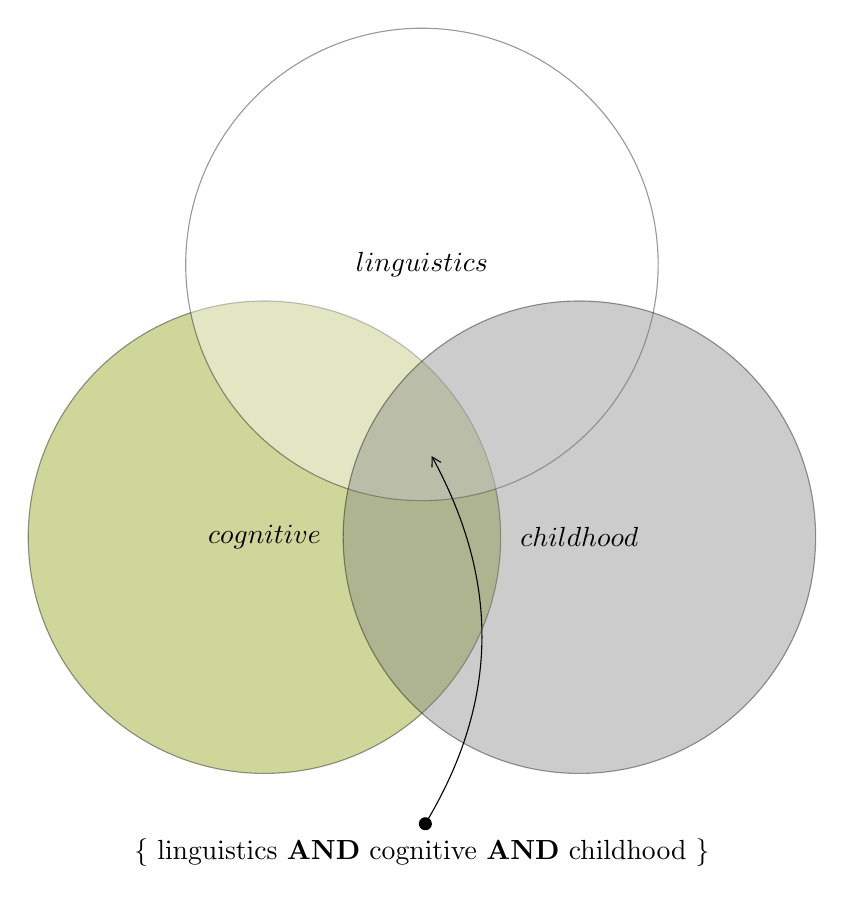
\begin{tikzpicture}
  \tikzset{venn circle/.style={draw,circle,minimum width=6cm,fill=#1,opacity=0.4,text opacity=1}}

  \node [venn circle = green] (A) at (0,0) {$cognitive$};
  \node [venn circle = white] (B) at (60:4cm) {$linguistics$};
  \node [venn circle = gray] (C) at (0:4cm) {$childhood$};
  \node[left] at (barycentric cs:A=1/2,B=1/2 ) {};
  \node[below] at (barycentric cs:A=1/2,C=1/2 ) {};
  \node[right] at (barycentric cs:B=1/2,C=1/2 ) {};
  \node at (barycentric cs:A=1/3,B=1/3,C=1/3 ) (endpoint) {};

  \draw[*-angle 60]
    ( [yshift=-20pt] $ (A.south)!0.5!(C.south) $ ) node[anchor=north] {\{ linguistics \textbf{AND} cognitive \textbf{AND} childhood \}}
    to[bend right,looseness=1]
    (endpoint.south east);
\end{tikzpicture}
%\begin{center} \includegraphics[width=.30\textwidth]{and3colors.png}
%\{ childhood \emph{AND} linguistics \emph{AND} cognitive \} \end{center}

\end{center}

\noindent In the search depicted above, a student has requested articles that
contain the  subjects \textbf{cognitive}, \textbf{linguistics}, and
\textbf{childhood}.  This particular search will only retrieve articles that
contain  \emph{all three terms}. This small subset of the larger subject sets is
referenced by the arrow. All the information represented by the other portions
of the three circles will be excluded. Thus, even if an article contains two of
the three search terms, it will be excluded from the results.

\subsection{OR} Unlike the \textbf{AND} operator, \textbf{OR} seeks to
\emph{broaden} a search,  as in this example:
\bigskip

\begin{center}
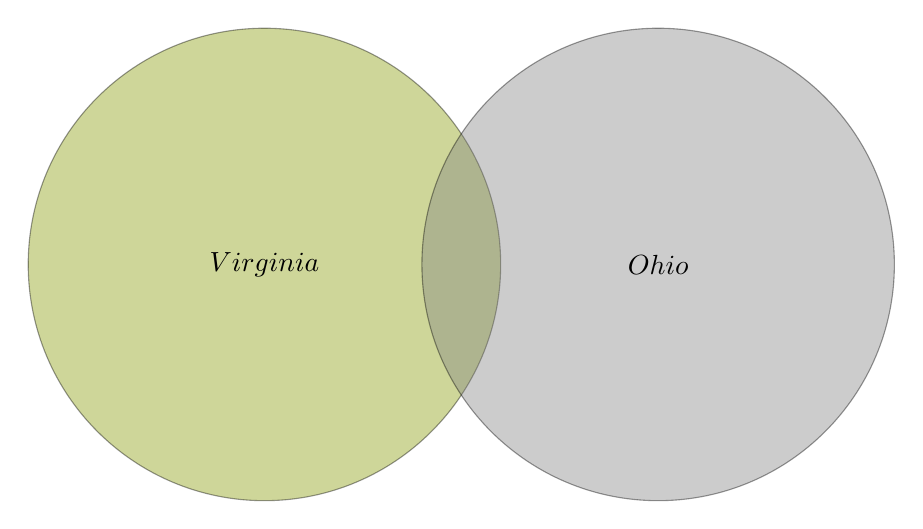
\begin{tikzpicture}
  [venn circle/.style={draw,circle,minimum width=6cm,fill=#1,opacity=0.4,text opacity=1}]

  \node [venn circle = green] (A) at (0,0) {$Virginia$};
  %\node [venn circle = white] (B) at (60:4cm) {$Ohio$};
  \node [venn circle = gray] (C) at (0:5cm) {$Ohio$};
  %\node[left] at (barycentric cs:A=1/2,B=1/2 ) {};

  \node[below] at (barycentric cs:A=1/3 ) (endpoint A) {};
  \node[below] at (barycentric cs:C=1/3 ) (endpoint C) {};

\end{tikzpicture}

\{ Virginia \textbf{OR} Ohio \}
\end{center}

%\begin{center} \includegraphics[width=.30\textwidth]{Orcolor.png}
%\{ Virginia \emph{or} Ohio \} \end{center}

\noindent In the search depicted above, a student has searched for the subjects
Virginia \textbf{OR} Ohio. This search will return \emph{every} article having
the  subject of Virginia as well as \emph{every} article with the subject of
Ohio.  Unlike the \textbf{AND} search, where only articles containing
\emph{both} terms are returned in the search results, the \textbf{OR} search
yields every source on both subjects regardless of whether those subjects
appear together in the same source. As a consequence, the \textbf{OR} search
will produce far more results.

\begin{itemize}\item Since the \textbf{OR} operator lacks precision, it is most
often used in parenthetical searches, described below.\end{itemize}

\subsection{NOT} The Boolean operator \textbf{NOT} is used to \emph{subtract} or
\emph{screen out} topics or keywords that are unwanted within the search
results.

\begin{center}

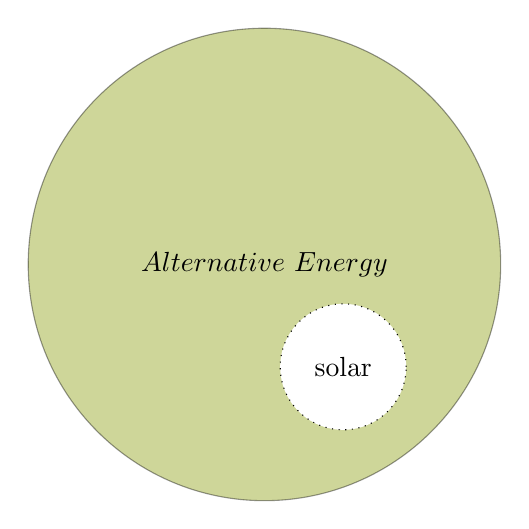
\begin{tikzpicture}
  \tikzset{venn circle/.style={draw,circle,minimum width=6cm,fill=#1,opacity=0.4,text opacity=1}}
  \node [venn circle = green] (A) at (0,0) {$Alternative \ Energy$};
  \path [draw=none,fill=white] (1,-1.3) circle (.8);
    \draw[dotted] (1,-1.3) circle (.8) node{solar};
    %\draw[solid] (0,-1) circle (2);
  %\node [venn circle = white] (B) at (60:4cm) {$Ohio$};
 % \node [venn circle = gray] (C) at (0:5cm) {$Ohio$};
  %\node[left] at (barycentric cs:A=1/2,B=1/2 ) {};
  %\node[below] at (barycentric cs:A=1/2,C=1/2 ) {};
  %\node[right] at (barycentric cs:B=1/2,C=1/2 ) {};
  %\node[below] at (barycentric cs:A=1/3 ) (endpoint) {};
 %  \node[below] at (barycentric cs:C=1/3 ) (endpoint) {};
  %\draw[*-angle 60]
   % ( [yshift=-10pt] $ (A.south)!0.5!(C.south) $ ) node[anchor=north] {\{ Virginia \emph{or} Ohio \}}
   % to[bend right,looseness=1.5]
   % (endpoint.south east);


\end{tikzpicture}


\{ alternative energy \textbf{NOT} solar \}

\end{center}

\noindent In the search depicted above, a student is researching alternative
energy and wants to exclude any information dealing with solar energy. To
remove all references to solar energy, the student has searched for
\textbf{alternative energy}, but has removed any articles from the search
results that contain the  subject \textbf{solar} using the operator
\textbf{NOT}.

The \textbf{NOT} operator is helpful when you find your search results are
"polluted" with unwanted items. This is often a problem when two distinct
things share the same name. For example, if you were researching the Norse
explorers known as the Vikings, you might discover that your search results
include unwanted information about the Minnesota Vikings football team. You can
subtract these unwanted results by searching for \textbf{Vikings NOT Minnesota}
or \textbf{Vikings NOT football}, for example.

\subsection{Parenthetical Searches}

You can also use the various Boolean search terms in tandem using parenthetical
constructions:

\begin{itemize} \item (Ohio OR Virginia) AND unemployment \item (cognitive AND
linguistics) NOT childhood \end{itemize} Such parenthetical searches follow the
order of operations, like in math  equations. In the first example, the search
will first combine all the articles  that are on the subjects of \textbf{Ohio}
or \textbf{Virginia}, creating a  large collection of search results. Afterward,
the search term  \textbf{unemployment} will be applied to that collection,
yielding the final search results. Similarly, the second example creates a
large collection of results that share the subjects \textbf{cognitive} and
\textbf{linguistics}, then all the items having the term \textbf{childhood}
are removed from the results.

\subsection{Exact Phrase Searches}

Most Internet search engines and library catalogs default to the \textbf{AND}
operator when multiple terms are entered, even if it has not been typed by the
user. For example, if you search for \textbf{artificial intelligence}, the
search algorithm will actually use the search phrase \textbf{artificial
\emph{and} intelligence} to produce your results. In some circumstances this
may produce undesirable or imprecise results. For example, we might imagine a scholarly article about the "intelligence" of using certain "artificial" sweeteners. This is not an article that is relevant for your research. 

To avoid this problem, you can instruct your search engine to perform what is
known as an \textbf{exact phrase search}. This is performed by placing
quotation marks around the exact words you are searching for. By searching
for "artificial intelligence" your search results will only contain items that
have that exact phrase within the document or title.

\subsection{Truncation and Wild Cards} \begin{itemize} \item manufact\**
[truncation] \item wom\**n [wild card] \end{itemize} If you search for the terms
\textbf{steel AND manufacturing}, your search  results may not include results
with the terms \textbf{manufacturer},  \textbf{manufacture},
\textbf{manufactured}, or \textbf{manufactures}. As a result, you may not
discover articles or books that are important to your research. By truncating
the word with an asterisk, you will gather all the relevant search results.

Similarly, if you only search for wom\hl{en}, you will potentially miss out on the
all the texts that mention wom\hl{an}. However, using the wild card
asterisk you will search both terms simultaneously, gathering all the results.

\section{Finding a Book in the Library}

\subsection{The Library of Congress System} Most research libraries use the
Library of Congress (LC) classification system to organize their holdings. The
Library of Congress assigns each book a unique \textbf{call number} consisting
of a series of numbers and letters that help  you locate them on the library's
shelves. A typical call number will resemble  the following:

\begin{center}
\bigskip

{\huge F 24 .T39 1990}
\end{center}

\bigskip

On a book's binding it will be written like this:

\begin{center}
{\huge F} \smallskip

{\huge 24}\smallskip

{\huge .T39}\smallskip

{\huge 1990}

\end{center}

\noindent Let's break down the call number into its component parts:

\bigskip

{\large
\begin{center}
\begin{tabular}{ ll }    \textbf{F} & Letter, or
subject, line \\    \textbf{24} & Whole number line \\     \textbf{.T39} & Cutter
line \\   \textbf{1990} & Edition, or Date, line\\  \end{tabular}
\end{center}
}
\medskip

\begin{itemize}

\item \textbf{The Letter line} describes the subject matter, or
discipline, of the book. It also indicates the section of the library where the
book is shelved (consult the library's \href{http://www.dartmouth.edu/~library/bakerberry/circ/stacksguides/}{floorplan
maps}). The letter line will be between one and three letters long. \item \textbf{The Whole number
line} tells you which \emph{row} the book is on in the stacks.  \item
\textbf{The Cutter line} identifies the \emph{individual book}. The first
letter of the Cutter line is usually the first letter of the author's last name.
\item \textbf{The Edition, or Date, line} tells you the book's year of
publication. This line is used to distinguish between editions.\bigskip

You can examine the \href{https://www.loc.gov/catdir/cpso/lcco/}{full list of subject classes} used by LC system online at the Library of Congress.\end{itemize}

\subsection{How to Find a Book} \smallskip

To find a book in the library, read the call number from left to right, using  alphabetical and
numerical orders. First, using the \textbf{Letter line},  determine the floor of
the library where the book is shelved. Use the library's
\href{http://www.dartmouth.edu/~library/bakerberry/circ/stacksguides/}{floorplan
maps}  to locate the proper section. Using our example call number above, we can
determine that the \textbf{F} section is in Stack Annex A.

Once on the appropriate floor, use the \textbf{Whole number line} to find the
row where the book is shelved in the stacks. Using the example call number, we
will look through the stacks for the number 24. The floormaps are often helpful
in locating the book's general location on the library floor. As you walk
through the stacks, look on the ends of each row of books for signs describing
the range of books held within the rows. There you will see signs like the one
pictured below.

\begin{center}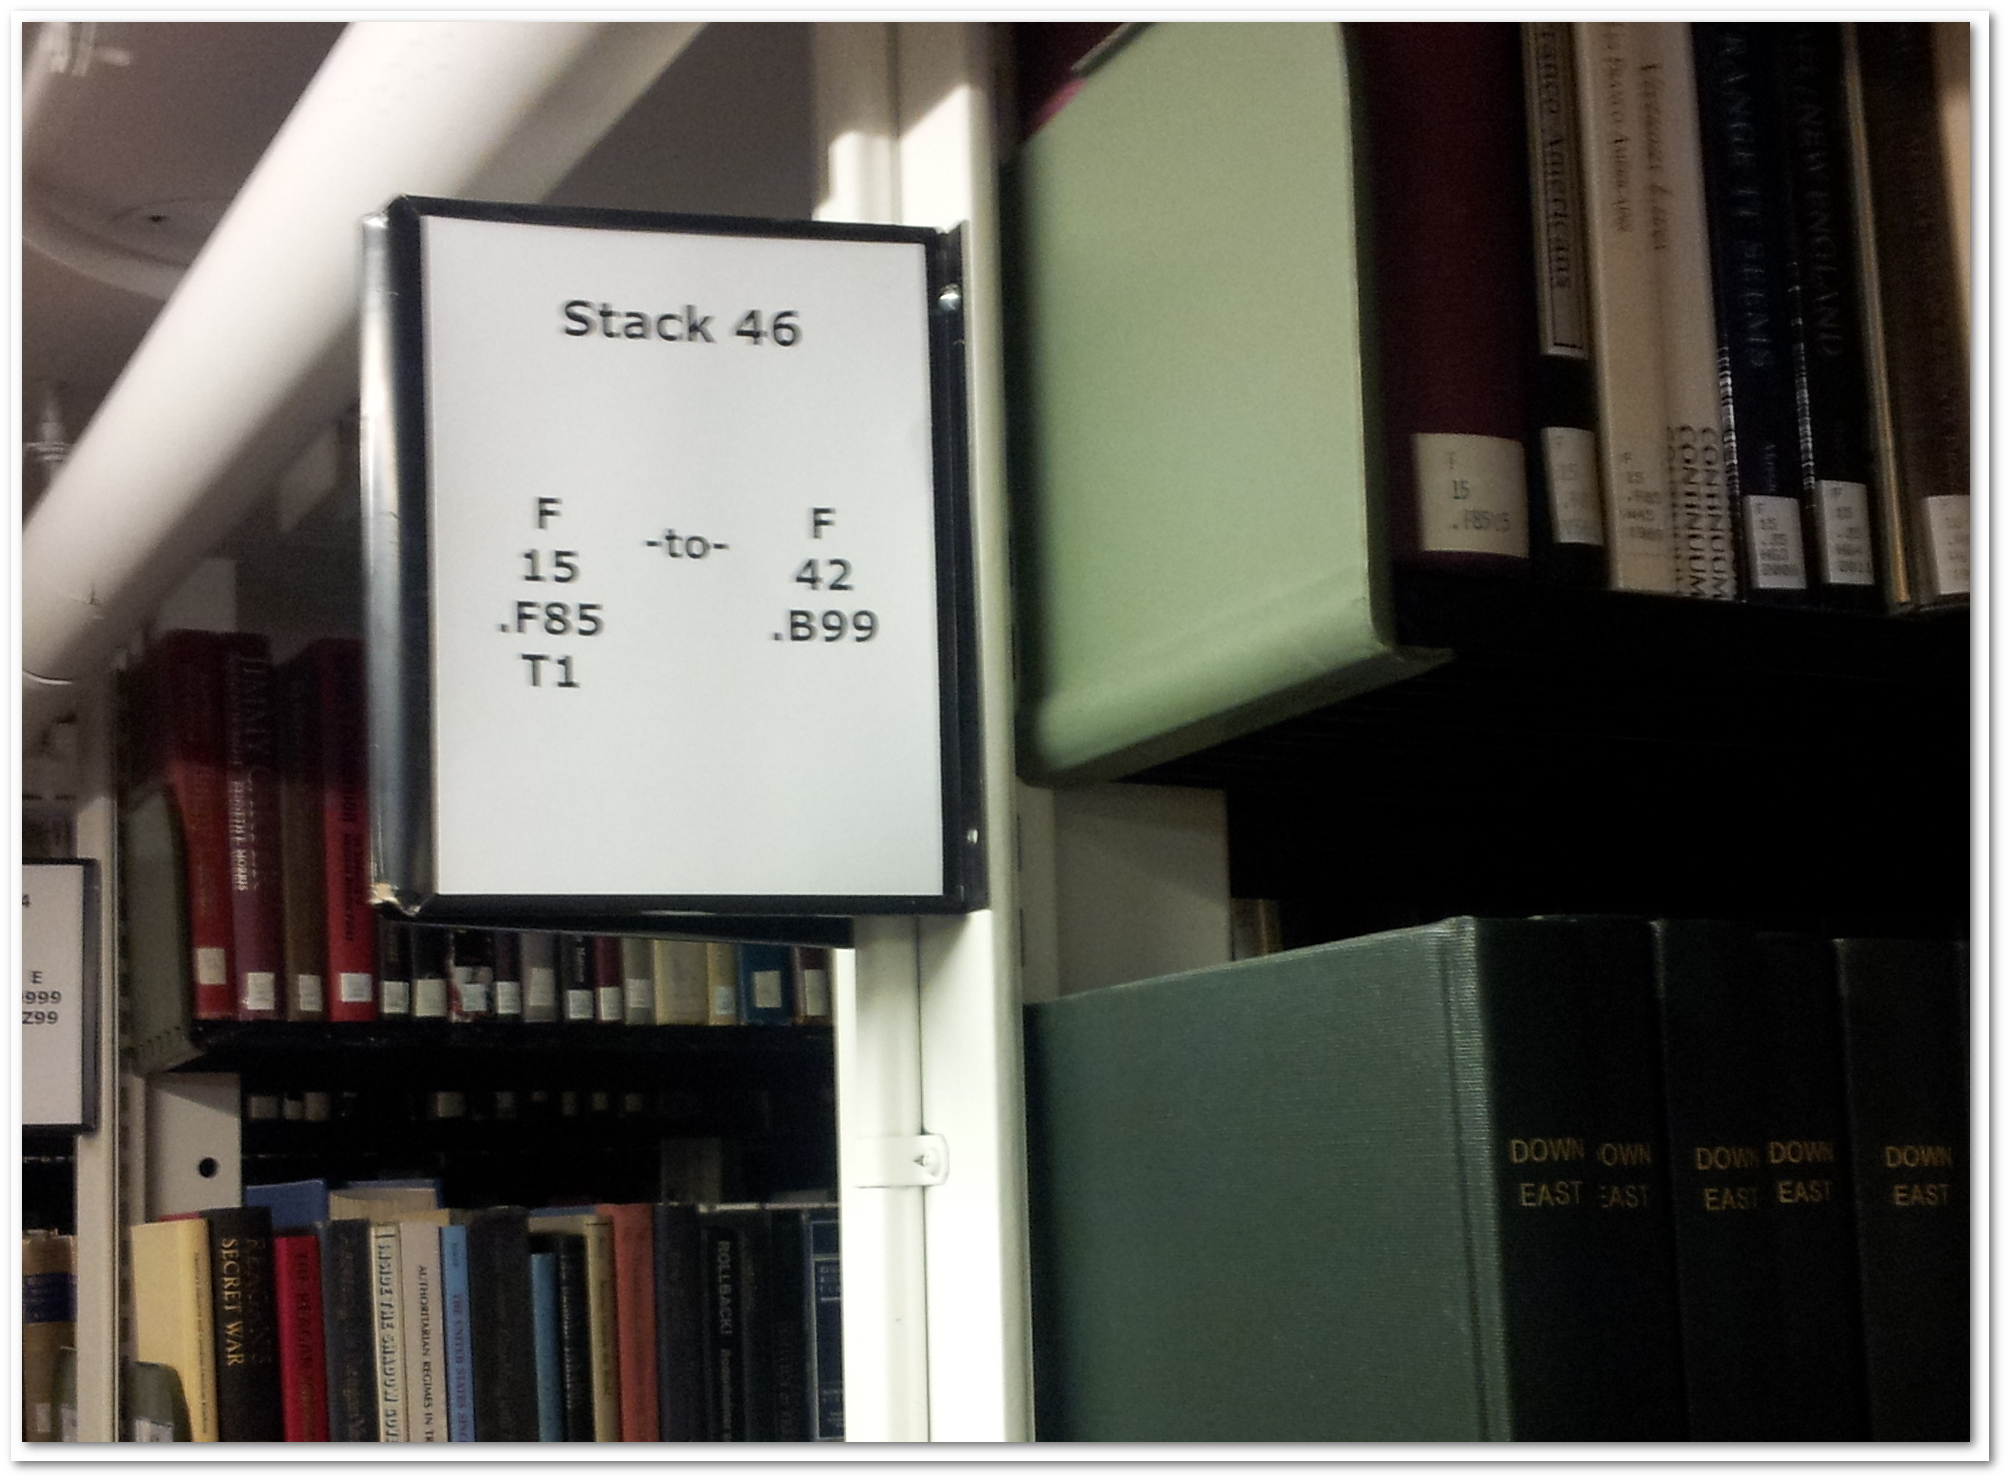
\includegraphics[scale=.15]{stacks}

{\small \{ \emph{Use these signs to determine if a book is in the row}. \}}

\end{center}



Since \textbf{F 24} is within this range, our example book is in that row. Once
in the proper row of shelves, proceed numerically until you find the 24s.
Finally, using the \textbf{Cutter line}, proceed alphabetically until you find
the Ts. Then proceed numerically until you find \textbf{.T39}, the address of our book.

As you can see, the call number should be read from left to right using
alphabetical and numerical orders. Thus, a book with a Subject line \textbf{F
}would be shelved \emph{before} a book with a Subject line \textbf{FA.}
Similarly, a Cutter line that reads \textbf{.T39} is shelved \emph{after}
\textbf{.T21}.

Maps of the library's floorplans are affixed to the walls on each floor. Free
paper maps of the library are available at the circulation desk of the library.
You may also consult the
\href{http://www.dartmouth.edu/~library/bakerberry/circ/stacksguides/}{maps and
floorplans} online with your computer or smartphone.

\begin{center}
\begin{tcolorbox}[colframe=oyster, coltitle=black, sharp corners, title=\ding{52} Note]
A new update to Dartmouth's catalog as of 2014
allows you to simply click the 
\includegraphics[scale=.6]{mapit} button next
to the item's listing. This will summon a map that shows you the exact location
of the book in the library stacks.
\end{tcolorbox}
\end{center}

\section{Sources our Library Doesn't Own}

A common problem in academic research is discovering that a book or article you
require for a project is checked out, missing, or not owned by the library.
There are a number of free services available to you when you encounter this
problem.

\subsection{Borrow Direct Consortium}

A number of the best libraries in the world have formed a consortium
designed to share resources and expand research opportunities for the  entire academic
community. As students of Dartmouth college, you may obtain  borrowing
privileges at any of the other participating libraries including Brown,
Columbia, Cornell, Harvard, Massachusetts Institute of Technology, University of
Chicago, University of Pennsylvania, Princeton, Yale and the Center for Research
Libraries. The combined resources total a staggering 50 million volumes.

To see if a book is available at another library, use a  service called
\href{http://www.dartmouth.edu/~library/res-share/borrowdirect/}{Borrow Direct}.
With this  service you may search every library in the consortium simultaneously
to see if the  book you require is available at another institution. If the book
is  owned by another school and is not checked out at the time, you may request
that the item be sent to our library. These requests usually arrive in 4 working
days or less.

\hypertarget{peer-review}{}

\subsection{DartDoc} If there is a book or article you would like to read that
is not available through Borrow Direct, you may request it from Dartmouth's
interlibrary loan program, known as DartDoc. To  request an item, visit the
\href{https://dartmouth.illiad.oclc.org/illiad/berry/logon.html}{DartDoc}
webpage, select the appropriate form (article, book, book chapter, etc.), and
send your request electronically to the office. Staff will
request your item from another library, who will ship the book to our library
through the mail. If you are requesting a book chapter or article, the donor
library will send you a .pdf free of charge to your DartDoc account.

\begin{center}
\begin{tcolorbox}[colframe=oyster, coltitle=black, sharp corners, title=\ding{52} Note]
If you are ordering a book, DartDoc is the
\emph{slowest} of all the  available options for requesting research materials.
Requests may take up to  two weeks to be fulfilled.
\end{tcolorbox}
\end{center}

\section{Research Guides}


If you are performing research on a topic and do not know where to begin,
Dartmouth's librarians have created an impressive collection of
\href{http://researchguides.dartmouth.edu}{Research Guides}  that can help you
find background information, periodical databases, and  academic journals
appropriate for your topic or discipline.


\section{Peer Review}

Peer review is a form of quality control in academic publishing. Before books
or articles are published, they experience a rigorous process of evaluation by
a number of experts who have advanced training in the field of study in
question. This scholarly review helps eliminate factual errors and other
problems before the works are published. Thus, peer-reviewed works are much more
trustworthy than other sources of information.

\subsection{Determining if a source is peer reviewed}

For novice researchers, distinguishing between \hyperlink{peer-review}{\color{Ahrenge}{peer-reviewed}} and other kinds of sources can be challenging. However, there are a number of things you can do to
ensure that you are using  peer-reviewed information. Many periodical databases,
such as  \href{http://dartmouth.idm.oclc.org/login?url=http://www.jstor.org/}{JSTOR}, only contain
peer-reviewed academic articles. Many other databases, such as
\href{http://dartmouth.idm.oclc.org/login?url=http://search.ebscohost.com/login.aspx?authtype=ip,uid&profile=ehost&defaultdb=a9h}{Academic
Search Complete}, have search limiters that can be selected to ensure  that the
search results only contain peer-reviewed sources. However, other  databases
lack clear indications about the nature of their sources. If you are  confused
about a source or database, ask your professor or one of the research
librarians for assistance.

If those are not practicable, use these test criteria: 

\begin{itemize} 

\item Scholarly, \hyperlink{peer-review}{\color{Ahrenge}{peer-reviewed}} articles almost always publish the university
affiliation of the professor/author/scientist.

\item Scholarly articles \emph{always} have a bibliography page.

\item Scholarly articles always contain citations and commonly have footnotes
or endnotes.

\item Generally speaking, if you can find the publication at the dentist's
office or on an airport magazine rack, then it isn't scholarly or
peer-reviewed. \emph{Time}, \emph{Newsweek}\textemdash even the \emph{New York
Times}\textemdash are not considered peer-reviewed sources. 

\item If the article contains advertisements, it is likely not scholarly. 

\end{itemize}

\section{The Oxford English Dictionary}

The \href{http://www.oed.com/}{OED} is, without question, the  greatest and most
complete dictionary ever created. As an historical dictionary, the OED systematically traces the  etymology of words in the English language.  \href{http://en.wikipedia.org/wiki/Etymology}{Etymology} is
"the study of the history of words, their origins, and how their form and
meaning have  changed over time." Thus, with the OED you can see when a word
entered or exited the English language and how its meaning evolved over time.

The OED is quite helpful when you are reading a novel, poem, or document that
was written in a time period distant from our own. Since words fall out of use
and the meanings of words change over time, it can often be difficult to
interpret the meaning of the texts we read from the past. The OED exists to
help us with this problem. You can think of it as a dictionary with a built-in
time machine.

\section{Helpful Research Suggestions}

\subsection{Not all sources are equal}

How do you know if you can trust your source? Here are some suggestions for
critically examining your sources:

\begin{itemize} \item \textbf{Examine the credentials of the author}. What is
the author's educational  background? Do they have an advanced degree in the
subject that they are  writing about? Are they affiliated with any major
institutions\textemdash such  as a university or government department? Does the
author have a respected  publication record that is frequently cited by other
experts in the field?

\item \textbf{Examine the date of publication}. When was the book or article
you are reading published? Since new discoveries and ideas are produced every
day, it is important to consult the most recent sources on your research
subject. Generally, the most current source should be preferred over older
sources.

\item \textbf{Determine if the source has been peer-reviewed}. Peer review is a
form of quality control in academic publishing. It ensures that the information
that is published has been properly evaluated and vetted by a number of other
professionals in the field. A peer-reviewed source should be preferred over any
other kind of information.

\item \textbf{Be wary of Internet sources}. If your source comes from the
Internet, you should take care to verify its trustworthiness. Most sites on the
Internet are not peer-reviewed sources of information. Misleading, politically
motivated, and even propagandistic content often masquerades as objective
information on blogs, websites, and discussion boards.  \end{itemize}

\subsection{Taking notes}

Now that you have some research materials in front of you, either at the
library or at home, it's time to make them useful to you. Before placing source
materials in your essay, \hyperlink{notes}{\color{Ahrenge}{take good notes}} by using \hyperlink{summary}{\color{Ahrenge}{summary}}, \hyperlink{paraphrase}{\color{Ahrenge}{paraphrase}}, and judicious \hyperlink{quotation}{\color{Ahrenge}{quotation}} to take ownership of the source materials. Ensure that
you cite appropriately and that your summaries and paraphrases use your own
original language. This intermediary step before writing the essay saves you
time and helps you avoid \hyperlink{plagiarism}{\color{Ahrenge}{plagiarism}}.

\begin{itemize}
\item If you'd like to keep organized notes on your computer, try the free and open-source
program called \href{http://rasm.ods.org/keepnote}{Keepnote}.
\end{itemize}

\subsection{Raid the Bibliography}

Occasionally, students find one or two sources on a topic and then despair of
finding any more. However, with just one excellent article or book, you can
easily generate additional research leads. When you find a book or article that
relates to your project, scour the bibliography to see what books and articles
the author used to produce his or her work. Make lists of the most promising
sources by writing down all the bibliographic information in a research
journal. Locate these sources in the library and then repeat the process. By
using this technique of routinely following up on sources cited in
bibliographies, you can generate a surprisingly large number of books and
articles on your topic in a relatively short time.

\subsection{Research Journal \& Bibliographic Software}

Keeping a research journal is an important habit to develop. Every student or
professor has had the unsettling realization that they have used a quotation in
their writing but have no recollection of where the quote came from. Many hours
can be consumed retracing steps. Frequently, source materials are never located
again. To avoid this problem, keep a research journal where you record the
bibliographic information of each source you read or browse. This way you can
quickly locate the information again.

Although a paper notebook works well as a research journal, there are some very
promising electronic alternatives. This bibliographic software can maintain a
record of your sources, help you take notes, and even produce perfectly
formatted bibliography pages for your essays.  \begin{itemize}\item For Mac
users, there is \href{http://www.sonnysoftware.com/}{Bookends}.  \item PC users
should consider \href{http://www.biblioscape.com}{Biblioscape}.  \item However,
the free and open-source option known as \href{http://zotero.org}{Zotero} is
perhaps the best option of all. \end{itemize}

%----------------------------------
% Common Sentence Errors
%-----------------------------------



\chapter{Common Sentence Errors}
\hypertarget{Top20}{}



A \href{http://www.jstor.org/stable/357695}{statistical study of student writing} performed in 1988 by scholars Andrea Lunsford and Robert Connors demonstrated that virtually all student
writing mistakes are limited to 20 formal errors. Eliminating these 
errors in your writing therefore offers the quickest path to error-free prose.

\setcounter{secnumdepth}{0}

\section{1. Missing comma after an introductory element}


\begin{itemize}
\item Similarly Freire argues that memorization as a form of education is dehumanizing. \ding{55}
\item Similarly, Freire argues that memorization as a form of education is dehumanizing. \ding{51}
\medskip
\item If the team wants to win they will have to practice more. \ding{55}
\item If the team wants to win, they will have to practice more. \ding{51}
\end{itemize}

\noindent Introductory words or clauses are usually set off with a comma.


\section{2. Wrong word} 
\begin{itemize}
\item The workmen assembled at the \hl{cite}. \ding{55}

\item The workmen assembled at the site. \ding{51}
\medskip
\item I have a bad case of \hl{ammonia}. \ding{55}

\item I have a bad case of pneumonia. \ding{51}
\end{itemize}


\section{3. Incomplete or missing documentation} 

\begin{itemize}
\item The response to the threat of terrorism should not be a curtailing of
freedoms. \ding{55}

\item The response to the threat of terrorism should not be a curtailing of
freedoms (Taylor 29). \ding{51}
\end{itemize}

\noindent Missing documentation for a quotation, summary, or paraphrase of another text
may result in charges of \hyperlink{plagiarism}{\color{Ahrenge}{plagiarism}}, a serious academic offense.

\section{4. Vague pronoun reference} 
\begin{itemize}
\item The teacher gave her notes to her. \ding{55}

\item The teacher gave her notes to Jane. \ding{51}
\end{itemize}


\section{5. Spelling error} 
\begin{itemize}
\item I \hl{definately} will be there. \ding{55}

\item I definitely will be there. \ding{51}
\end{itemize}


\section{6. Faulty Parallelism} 
\begin{itemize}
\item He was good at swearing, fighting, and liked to drink. \ding{55}
\item He was good at swearing, fighting, and drinking. \ding{51}
\smallskip

\item They were informed that they should not eat before swimming, that they should not eat sugar, and to do some exercises before bed. \ding{55}

\item They were informed that they should not eat before swimming, that they should not eat sugar, and that they should not skip exercise before bed. \ding{51}

\end{itemize}

\noindent Parallel structure involves using the same form of words or structural pattern when crafting a sentence. In the example above, the author uses gerunds for the first two verbs but then changes to the infinitive form for the last verb. Generally, parallel structure sounds much better to the ear than otherwise. 


\section{7. Unnecessary comma} 
\begin{itemize}
\item The legal language applies to carnivals, and to amusement parks.  \ding{55}

\item The legal language applies to carnivals and to amusement parks.  \ding{51}
\end{itemize}
\medskip
\begin{itemize}
\item The cemetery on the hill, is haunted. \ding{55}

\item The cemetery on the hill is haunted. \ding{51}
\end{itemize}
\medskip
\begin{itemize}
\item The man, who held the American flag, waved to us from the tour bus.  \ding{55}

\item The man who held the American flag waved to us from the tour bus.  \ding{51}
\end{itemize}

\noindent The phrase "who held the American flag" is a \emph{restrictive} element: a part of a sentence that is essential its meaning. This information identifies the particular man who waved from all the others on the bus. Restrictive elements are \emph{never} set off with commas. 


\section{8. Missing comma with a nonrestrictive element} 

\begin{itemize}
\item Jeff who owned the corporation was a big gambler and a cheat. \ding{55}

\item Jeff, who owned the corporation, was a big gambler and a cheat. \ding{51}
\end{itemize}

\noindent A \textbf{nonrestrictive element} is a part of a sentence that is not essential to its
meaning. Commas are used to set off these nonessential portions of the
sentence.


\section{9. Missing comma in compound sentence} 

\begin{itemize}
\item I've given him all that I own and I can't see myself giving more. \ding{55}

\item I've given him all that I own, and I can't see myself giving more. \ding{51}
\end{itemize}

\noindent A compound sentence contains two or more clauses that can stand alone as
complete sentences (otherwise known as "independent clauses"). However,
to connect them you must either use a semicolon or use a comma and
coordinating conjunction such as \emph{and}, \emph{but}, or \emph{yet}. Failing
to punctuate the compound sentence results in a \textbf{fused}, or \textbf{run-on}, sentence.


\section{10. Faulty sentence structure} 
\begin{itemize}
\item With so much going on in the world today is why it is so hard to 
keep up with everything. \ding{55}

\item With so much going on in the world, it can be hard to keep up. \ding{51}
\end{itemize}

\noindent When a sentence begins with a certain structure, then abruptly shifts to a different
one, it becomes disorderly and difficult to follow. 



\section{11. Unnecessary shift in verb tense} 
\begin{itemize}
\item She ran to the store and picks up some milk. \ding{55}

\item She ran to the store and picked up some milk. \ding{51}
\end{itemize}

\section{12. Lack of agreement between pronoun and antecedent}

\begin{itemize}
\item Each of the prisoners found happiness in their work. \ding{55}

\item Each of the prisoners found happiness in his work. \ding{51}
\medskip
\item Either Jeff or Robert will be required to give up their car. \ding{55}

\item Either Jeff or Robert will be required to give up his car. \ding{51}
\medskip
\item The campaign constantly changed its positions in the weeks before the election. \ding{51}

\item The campaign constantly changed their positions in the weeks before the election. \ding{51}
\end{itemize}

\noindent Pronouns and their antecedents must always agree in number. Three 
rules govern the choice between singular or plural pronouns. 1) Sentences that begin
with an indefinite pronoun (such as everyone and each) are \emph{always}
treated as singular. 2) If antecedents are joined by \emph{or} or \emph{nor}, 
the pronoun must agree with the \emph{closer} antecedent. 3) Collective nouns can be either 
singular or plural depending on whether the people are seen as a single unit or a 
group of individuals.

\section{13. Missing or misplaced possessive apostrophe} 

\begin{itemize}
\item The Baker Hill farm stand is proud to offer \hl{it's} vegetables for sale now. \ding{55}

\item The Baker Hill farm stand is proud to offer its vegetables for sale now. \ding{51}
\medskip
\item The Indian's best player is Ubaldo Jimenez. \ding{55}

\item The Indians' best player is Ubaldo Jimenez. \ding{51}
\end{itemize}

\section{14. It's / Its error} 


\begin{itemize}
\item Its unfair to make him pay for all the damages. \ding{55}

\item It's unfair to make him pay for all the damages. \ding{51}
\end{itemize}

\noindent\textbf{It's} is a contraction and means "it is" or "it has." \textbf{Its} is the
possessive form of it.

\section{15. Fused (run-on) sentence} 

\begin{itemize}
\item Jeff was Wisconsin's greatest dog trainer he could make a canine do virtually anything. \ding{55}

\item Jeff was Wisconsin's greatest dog trainer; he could make a canine do virtually anything \ding{51}
\end{itemize}

\noindent A fused sentence is also known as a "run-on" sentence. It occurs when two
clauses that could stand alone as complete sentences are placed together
without punctuation.


\section{16. Comma splice} 

\begin{itemize}
\item Indians once ruled the valley, they are all gone now. \ding{55}

\item Indians once ruled the valley, but they are all gone now. \ding{51}

\item Indians once ruled the valley; they are all gone now. \ding{51}
\end{itemize}

\noindent A comma splice occurs when two independent clauses are joined by a comma. To
revise, use a comma with a coordinating conjunction or a semicolon.



\section{17. Misplaced modifier}
\begin{itemize}
\item He wore his new coat to church, which was covered in cat hair. \ding{55}

\item He wore his new coat, which was covered in cat hair, to church. \ding{51}
\end{itemize}

\noindent The first example suggests that the church, rather than the coat, was covered in cat hair.




\section{18. Poorly integrated quotation} 

\begin{itemize}
\item Scholar Rod Andrews argues "I argue that there can be no 
reasonable discussions of Shakespeare's biography" (99). \ding{55}

\item Scholar Rod Andrews argues that "there can be no reasonable discussions 
of Shakespeare's biography" (99). \ding{51}
\end{itemize}

\noindent When you integrate borrowed material into your own writing, the 
"hybrid" sentence you create must satisfy grammar. Further, the quoted material should
blend seamlessly into your sentence structure.

\section{19. Unnecessary or missing hyphen} 
\begin{itemize}
\item He bought a nineteenth century painting. \ding{55}

\item He bought a nineteenth-century painting. \ding{51}

\item Boston has a lot of one way streets. \ding{55}

\item Boston has a lot of one-way streets. \ding{51}
\end{itemize}

\section{20. Sentence fragment}

\begin{itemize}
\item This school offers many classes. Such as Accounting and English. \ding{55}

\item This school offers many classes, such as Accounting and English. \ding{51}
\end{itemize}

\noindent A fragment is an incomplete thought. It is a dependent clause treated
as an independent clause.

%

\chapter{Comment Buttons}
\hypertarget{commentbuttons}{}

\newcommand\invisiblesection[1]{%
\refstepcounter{section}%
\addcontentsline{toc}{section}{\protect\numberline{\thesection}#1}%
\sectionmark{#1}}

\iconsectioninToC  


There is
\href{http://www.inventio.us/ccc/1988/12/robert-j-connors-and-andrea-a.html}{strong
statistical evidence} that almost 100\% of student writing problems are limited
to 20 discrete errors. As a result, I find myself writing the same things over
and over (and over) at the expense of more substantive remarks. I developed
Comment Buttons™ as a way of speeding up this process.

Comment Buttons™ are a kind of shorthand\textemdash a system of symbols representing
specific errors that I quickly jot into the margins of student writing. Later,
you may “decode” the symbols with the documentation below. Pay close attention
to the codes you generate; they will help you become more aware of the specific
problems you have in your writing and will thus help you to eliminate them.

An additional benefit of Comment Buttons™ is that it requires you to take
ownership of the revision process. Rather than merely retyping what I have
written on the pages of your essay, you must thoughtfully examine the
grammatical rules and examples yourself, then make appropriate revisions to your
work.\\

\invisiblesection{Audience} \begin{center}

\resizebox{1.5cm}{1.5cm}{%

\begin{tikzpicture}[scale=4, transform shape]
\tikzstyle{every node} = [circle, circular drop shadow, fill=Ahrenge!80]
\node (a) at (0, 0) {A};
	
\end{tikzpicture}
}

\bigskip

{\huge 1. Audience} \end{center}

It is important that you carefully consider the intended audience of your
writing. If your essay makes use of other texts, theories, or ideas, it is
important that you properly introduce them and provide appropriate context. As
you write, pretend that your audience is someone who is not taking part in our
class. What context do you need to provide your audience with so that your
ideas/thesis will make sense? For more advice on this subject,
visit the \hyperlink{audience}{\color{Ahrenge}{chapter on audience}} in this handbook.

\invisiblesection{Wow!} \begin{center}
\resizebox{1.5cm}{1.5cm}{%

\begin{tikzpicture}[scale=4, transform shape]
\tikzstyle{every node} = [circle, circular drop shadow, fill=Ahrenge!80]
\node (a) at (0, 0) {!};
	
\end{tikzpicture}
}

\bigskip


{\huge 2. Wow!} \end{center}

This button indicates that you have made an unusually sharp and penetrating
thought, idea, or claim. It might also indicate a fantastic turn of phrase or
beautiful and fluid moment of expression. Since this idea, observation, or
argument was so wonderful, you might consider whether you should expand on it a
bit, or otherwise make it a more central feature of your essay.

\invisiblesection{Uh, What?} \begin{center}
\resizebox{1.5cm}{1.5cm}{%

\begin{tikzpicture}[scale=3, transform shape]
\tikzstyle{every node} = [circle, circular drop shadow, fill=Ahrenge!80]
\node (a) at (0, 0) {?};
	
\end{tikzpicture}
}

\bigskip


{\huge 3. Uh, What?} \end{center}

This button refers to a statement that is confusing, ambiguous, or awkwardly
phrased. If reading the passage out loud to yourself does not reveal the problem
to you, please come by and see me for an explanation.

\invisiblesection{Add Space} \begin{center}
\resizebox{1.5cm}{1.5cm}{%

\begin{tikzpicture}[scale=4, transform shape]
\tikzstyle{every node} = [circle, circular drop shadow, fill=Ahrenge!80]
\node (a) at (0, 0) {\#};
	
\end{tikzpicture}
}
\bigskip

{\huge 4. Add Space} \end{center}

This symbol is a common copywriter’s mark that simply means to \emph{add a
space} between two letters or some punctuation. For example, if you write
“everyday,” as one word but mean “every day,” as two words, I will place this
mark in the margin and draw a line to the place where the space should be added.

\invisiblesection{Colloquial Language} \begin{center}
\resizebox{1.5cm}{1.5cm}{%

\begin{tikzpicture}[scale=3, transform shape]
\tikzstyle{every node} = [circle, circular drop shadow, fill=Ahrenge!80]
\node (a) at (0, 0) {CL};
	
\end{tikzpicture}
}

\bigskip


{\huge 5. Colloquial Language} \end{center}

Colloquial language is a fancy term that means common or everyday speech. Slang,
for example, is considered colloquial language. You should avoid common speech
or slang in your formal writing assignments. You want your audience to see you
as a scholar who speaks with authority and knowledge. For example, words like
“shady” or “ginormous” are better rendered “conspicuous” and “commodious.”

\invisiblesection{Close Space} \begin{center}
\resizebox{1.5cm}{1.5cm}{%
\begin{turn}{90}

\begin{tikzpicture}[scale=3, transform shape]
\tikzstyle{every node} = [circle, circular drop shadow, fill=Ahrenge!80]
\node (a) at (0, 0) {( )};
	
\end{tikzpicture}
\end{turn}
}
\bigskip


{\huge 6. Close Space} \end{center}

This indicates that you should close the space between two words or punctuation
marks. For example, I may draw this symbol when you write “every day” as two
words but meant to use the word “everyday,” as one word.

\invisiblesection{Citation Error} \begin{center}
\resizebox{1.5cm}{1.5cm}{%

\begin{tikzpicture}[scale=3, transform shape]
\tikzstyle{every node} = [circle, circular drop shadow, fill=Ahrenge!80]
\node (a) at (0, 0) {C};
	
\end{tikzpicture}
}
\bigskip

{\huge 7. Citation} \end{center}

This button indicates that there is an error in your citation. Either there is a
need for a citation or the citation is improperly formatted. If you are confused
about citation, investigate the matter in the chapters on citation and working
with sources (or ask me for an explanation).

\invisiblesection{ESL} \begin{center}
\resizebox{1.5cm}{1.5cm}{%

\begin{tikzpicture}[scale=3, transform shape]
\tikzstyle{every node} = [circle, circular drop shadow, fill=Ahrenge!80]
\node (a) at (0, 0) {ESL};
	
\end{tikzpicture}
}

\bigskip

{\huge 8. ESL} \end{center}

Some students are actually \emph{far more advanced} than their American
counterparts: they are taking this class in their \emph{second} language. This
button indicates a place where you have used non-standard English or have made a
common mistake for ESL writers.

\invisiblesection{Capitalize} \begin{center}
\resizebox{1.5cm}{1.5cm}{%

\begin{tikzpicture}[scale=4, transform shape]
\tikzstyle{every node} = [circle, circular drop shadow, fill=Ahrenge!80]
\node (a) at (0, 0) {\underline{\underline{a}}};

\end{tikzpicture}
}
\bigskip

{\huge 9. Capitalize} \end{center}

Generally, this is just an error in proofreading. This button means to
capitalize the underlined letter.

\invisiblesection{Discuss with Me} \begin{center}
\resizebox{1.5cm}{1.5cm}{%

\begin{tikzpicture}[scale=4, transform shape]
\tikzstyle{every node} = [circle, circular drop shadow, fill=Ahrenge!80]
\node (a) at (0, 0) {D};

\end{tikzpicture}
}

\bigskip

{\huge 10. Discuss with Me} \end{center}

Some things are too complicated to be placed in the margins of your essay. This
button merely invites you to discuss the issue with me after class or during an
office hour. I am happy to explain things in more detail.

\invisiblesection{Grammar Error} \begin{center}
\resizebox{1.5cm}{1.5cm}{%
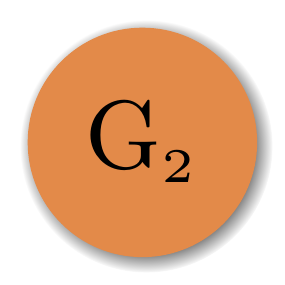
\begin{tikzpicture}[scale=3.5, transform shape]
\tikzstyle{every node} = [circle, circular drop shadow, fill=Ahrenge!80]
\node (a) at (0, 0) {G\textsubscript{\tiny 2}};

\end{tikzpicture}
}

\bigskip

{\huge 11. Grammar Error} \end{center}

This button indicates that you have made a grammatical error of some sort. If
there is a number included in the button, it corresponds to the list of the
\hyperlink{Top20}{\color{Ahrenge}{Twenty Most Common Errors}} in the previous
chapter. Consult the previous chapter for a description of the error and revise
appropriately: 1) Missing comma after an introductory element; 2) Wrong word; 3)
Incomplete or missing documentation; 4) Vague pronoun reference; 5) Spelling
error (including homonyms); 6) Faulty parallelism; 7) Unnecessary comma; 8)
Missing comma with a nonrestrictive element; 9) Missing comma in compound
sentence; 10) Faulty sentence structure; 11) Unnecessary shift in verb tense;
12) Lack of agreement between pronoun and antecedent; 13) Missing or misplaced
possessive apostrophe; 14) Its/It's error; 15) Fused (run-on) sentence; 16)
Comma splice; 17) Misplaced modifier; 18) Poorly integrated quotation; 19)
Unnecessary or missing hyphen; 20) Sentence fragment.


\bigskip

\invisiblesection{Strike} \begin{center}
\resizebox{1.5cm}{1.5cm}{%

\begin{tikzpicture}[scale=4,transform shape]
\tikzstyle{every node} = [circle, circular drop shadow, fill=Ahrenge!80]
\node (a) at (0, 0) {\cancel {B}};
	
\end{tikzpicture}
}
\bigskip

{\huge 12. Strike} \end{center}

This button has two meanings: 1) It may mean to remove the textual element that
is marked out—this might be a letter, word, or punctuation mark. 2) However, it
may also be used to suggest a change from an uppercase to lowercase letter.

\invisiblesection{Interpretation Problem} \begin{center}
\resizebox{1.5cm}{1.5cm}{%

\begin{tikzpicture}[scale=4, transform shape]
\tikzstyle{every node} = [circle, circular drop shadow, fill=Ahrenge!80]
\node (a) at (0, 0) {I};
	
\end{tikzpicture}
}
\bigskip


{\huge 13. Interpretation} \end{center}

This indicates that you have made an error in the interpretation of the source
material. For example, you might claim that an author argues for X when in fact
he or she argues the opposite.

\begin{center} 
\resizebox{1.5cm}{1.5cm}{%

\begin{tikzpicture}[scale=4, transform shape]
\tikzstyle{every node} = [circle, circular drop shadow, fill=Ahrenge!80]
\node (a) at (0, 0) {L};
	
\end{tikzpicture}
}
\bigskip

\invisiblesection{Logic} {\huge 14. Logic} \end{center}

This button indicates that there is a logical inconsistency in your writing.
Most often this involves a “leap” in logic or an unexpected or disruptive turn
in your writing that creates confusion. This might also involve an argumentative
statement that you make that seems to contradict an earlier one. At worst, it
might involve a line of reasoning or a statement that contradicts your thesis
statement.

\invisiblesection{Punctuation Error} \begin{center}
\resizebox{1.5cm}{1.5cm}{%

\begin{tikzpicture}[scale=3, transform shape]
\tikzstyle{every node} = [circle, circular drop shadow, fill=Ahrenge!80]
\node (a) at (0, 0) {P};
	
\end{tikzpicture}
}
\bigskip

{\huge 15. Punctuation Error} \end{center}

This button indicates that you have either misused punctuation or have left some
needful punctuation out. Consult your handbook for help with the punctuation
error or ask me for help.

\invisiblesection{Quotation Error} \begin{center}
\resizebox{1.5cm}{1.5cm}{%

\begin{tikzpicture}[scale=3, transform shape]
\tikzstyle{every node} = [circle, circular drop shadow, fill=Ahrenge!80]
\node (a) at (0, 0) {{\fixproblemfont Q}\textsubscript{\tiny 2}};

\end{tikzpicture}
}
\bigskip

{\huge 16. Quotation Error} \end{center}

This button indicates a problem with the integration of quotations. Like the
grammar button above, quotation errors will be identified with the following
numbers: 1) \textbf{Grammar}: The integration of the quotation creates a
grammatical error in the sentence of which it is a part. 2) \textbf{Logic}: The
quote has no clear relationship to the argument you are attempting to make or
illustrate. 3) \textbf{No introduction}: The quote is not introduced. Use a
signal phrase or otherwise weave the quote into your own writing. Avoid merely
plopping stand-alone quotations into your own writing. 4) \textbf{No
explanation}: Readers want to know \emph{why} you've quoted another writer's
words. What is significant about this quote? How is it relevant to your thesis
or overall project? 5) \textbf{Error with alteration}: There is a problem with
ellipsis [. . .] or [brackets] to indicate an omission or addition. 6)
\textbf{Lack of flow}: The quotation does not flow with the text that appears
before it, creating a sudden shift in voice, emphasis, topic, or tone. 7)
\textbf{No justification}: Quotes must be justified. If the quote you use
contains only factual information or uses language that is ordinary, there is no
need to quote it. Instead, put the idea or facts into your own words and then
cite the author.

\invisiblesection{Repetitive} \begin{center}
\resizebox{1.5cm}{1.5cm}{%

\begin{tikzpicture}[scale=3, transform shape]
\tikzstyle{every node} = [circle, circular drop shadow, fill=Ahrenge!80]
\node (a) at (0, 0) {R};
	
\end{tikzpicture}
}
\bigskip

{\huge 17. Repetitive} \end{center}

This button indicates a repeated word, concept, or idea. It might also involve
something that you say over and over again. Also, you might do something
redundant, like reiterate the same thing a few times using only slightly
different language.

\invisiblesection{Subject/Verb Agreement} \begin{center}
\resizebox{1.5cm}{1.5cm}{%

\begin{tikzpicture}[scale=4, transform shape]
\tikzstyle{every node} = [circle, circular drop shadow, fill=Ahrenge!80]
\node (a) at (0, 0) {S/V};

\end{tikzpicture}
}
\bigskip

{\huge 18. Subject/Verb Agreement} \end{center}

This indicates that your subject and verb do not agree in number. Both must be
singular or both must be plural.

\invisiblesection{Topic Sentence} \begin{center}
\resizebox{1.5cm}{1.5cm}{%

\begin{tikzpicture}[scale=3, transform shape]
\tikzstyle{every node} = [circle, circular drop shadow, fill=Ahrenge!80]
\node (a) at (0, 0) {TS};

\end{tikzpicture}
}
\bigskip

{\huge 19. Topic Sentence} \end{center}

Topic sentences are very important in academic writing. A topic sentence
functions as a “mini thesis” that announces the subject of a paragraph. As you
revise your writing, ensure that you have strong, descriptive topic sentences
and that the paragraphs that follow are unified under that topic or idea. For
those of you who have difficulties with organization, revising topic sentences
and checking paragraphs for unity is the fastest route to improvement.

\invisiblesection{Transitions} \begin{center}
\resizebox{1.5cm}{1.5cm}{%

\begin{tikzpicture}[scale=3, transform shape]
\tikzstyle{every node} = [circle, circular drop shadow, fill=Ahrenge!80]
\node (a) at (0, 0) {T};
	
\end{tikzpicture}
}
\bigskip

{\huge 20. Transitions} \end{center}

This button indicates a jarring or unexpected transition or sudden “leap” into
another subject. This often occurs between paragraphs, but may just as easily
occur between sentences if you suddenly change topic or emphasis. Sudden shifts
of focus such as this carry a very negative rhetorical consequence: it makes you
appear careless or illogical to your readers.

\invisiblesection{Spelling} \begin{center}
\resizebox{1.5cm}{1.5cm}{%

\begin{tikzpicture}[scale=3, transform shape]
\tikzstyle{every node} = [circle, circular drop shadow, fill=Ahrenge!80]
\node (a) at (0, 0) {S};
	
\end{tikzpicture}
}
\bigskip

{\huge 21. Spelling} \end{center}

This button indicates misspelled word. It may also include a "wrong word error"
where a word is spelled correctly, but is not the intended word. For example, "I
will \hl{meat} you after school." Sounds dreadful!

\invisiblesection{Word Choice} \begin{center}
\resizebox{1.5cm}{1.5cm}{%

\begin{tikzpicture}[scale=3, transform shape]
\tikzstyle{every node} = [circle, circular drop shadow, fill=Ahrenge!80]
\node (a) at (0, 0) {WC};
\end{tikzpicture}
}
\bigskip

{\huge 22. Word Choice} \end{center}

This indicates a word choice error. Commonly, the word in question has a
definition that is inconsistent with the meaning you intend or is otherwise
counterproductive to the meaning you intend. The best thing to do here is to
look up the word in a dictionary to examine its meaning(s). Additionally, I may also use this symbol if the word in question may create a
problem for your audience or argument. For example, calling someone “brain-dead”
or a “midget” might offend your readers. This might also involve the lack of
inclusive, \href{http://www.ncte.org/positions/statements/genderfairuseoflang}{gender-fair language}. An example of this would be the overuse of the
pronoun “he” to refer to a generic person or the use of “man” to signify both
women and men.

\invisiblesection{Unified Paragraph} \begin{center}
\resizebox{1.5cm}{1.5cm}{%

\begin{tikzpicture}[scale=3, transform shape]
\tikzstyle{every node} = [circle, circular drop shadow, fill=Ahrenge!80]
\node (a) at (0, 0) {UP};
	
\end{tikzpicture}
}
\bigskip

{\huge 23. Unified Paragraph} \end{center}

This indicates that your paragraph is not unified under a single topic. You
should have a clear topic sentence and what follows in the paragraph should be
focused on that one idea. Generally, this button appears when paragraphs contain
multiple ideas or shifts in focus.

\invisiblesection{Italicize} \begin{center}
\resizebox{1.5cm}{1.5cm}{%

\begin{tikzpicture}[scale=3, transform shape]
\tikzstyle{every node} = [circle, circular drop shadow, fill=Ahrenge!80]
\node (a) at (0, 0) {/  /};
	
\end{tikzpicture}
}
\bigskip

{\huge 24. Italicize} \end{center}

The forward slashes on either side of a word indicates that it should be
\emph{italicized}. For example, you may have forgotten to italicize the title of
a book or the name of a journal as required by your citation style.
Alternatively, italics may also be used for emphasis, which asks your readers to
give more weight to a particular word in your writing. While this can be very
effective, it should be used \emph{sparingly}.

\newpage

\invisiblesection{New Paragraph} \begin{center}
\resizebox{1.5cm}{1.5cm}{%

\begin{tikzpicture}[scale=4, transform shape]
\tikzstyle{every node} = [circle, circular drop shadow, fill=Ahrenge!80]
\node (a) at (0, 0) {\fixproblemfont\P~};
\end{tikzpicture}
}
\bigskip


{\huge 25. New Paragraph} \end{center}

This symbol, known as a "pilcrow," means to begin a new paragraph. This
indicates a moment in your writing when it appears that you have begun a new
idea or changed focus such that a new paragraph is warranted.

\invisiblesection{Insert} \begin{center}
\resizebox{1.5cm}{1.5cm}{%

\begin{tikzpicture}[scale=4, transform shape]
\tikzstyle{every node} = [circle, circular drop shadow, fill=Ahrenge!80]
\node (a) at (0, 0) {\textasciicircum};
\end{tikzpicture}
}
\bigskip

{\huge 26. Insert} \end{center}

This symbol, known as a "caret," indicates that I have added a word or some
language to one of your sentences. This addition should be considered, not
automatically adopted. This is \emph{your} essay, after all.

\invisiblesection{Problem Area} \begin{center}

\resizebox{1.5cm}{1.5cm}{%

\begin{tikzpicture}
\fill[fill=Ahrenge!80, circular drop shadow] (0,0) circle (1cm);

\draw[line width=1pt, color=black] plot [domain=-.85:.85, samples=30, smooth] (\x,{0.1*rand});
\end{tikzpicture}
}
\bigskip

{\huge 27. Problem Area} \end{center}

This squiggly line will appear beneath the specific text that contains a
grammatical error, confusing statement, formatting concern, or other type of
problem. Look in the margin next to these marks for an explanation or comment.

\stdsectioninToC 





\end{document}
